\chapter{
  Additional Figures
 }

\clearpage
\section{
  Control Region DY+Jets Boosted ZV Channel
 }

\begin{figure}[!ht]
  \centering
  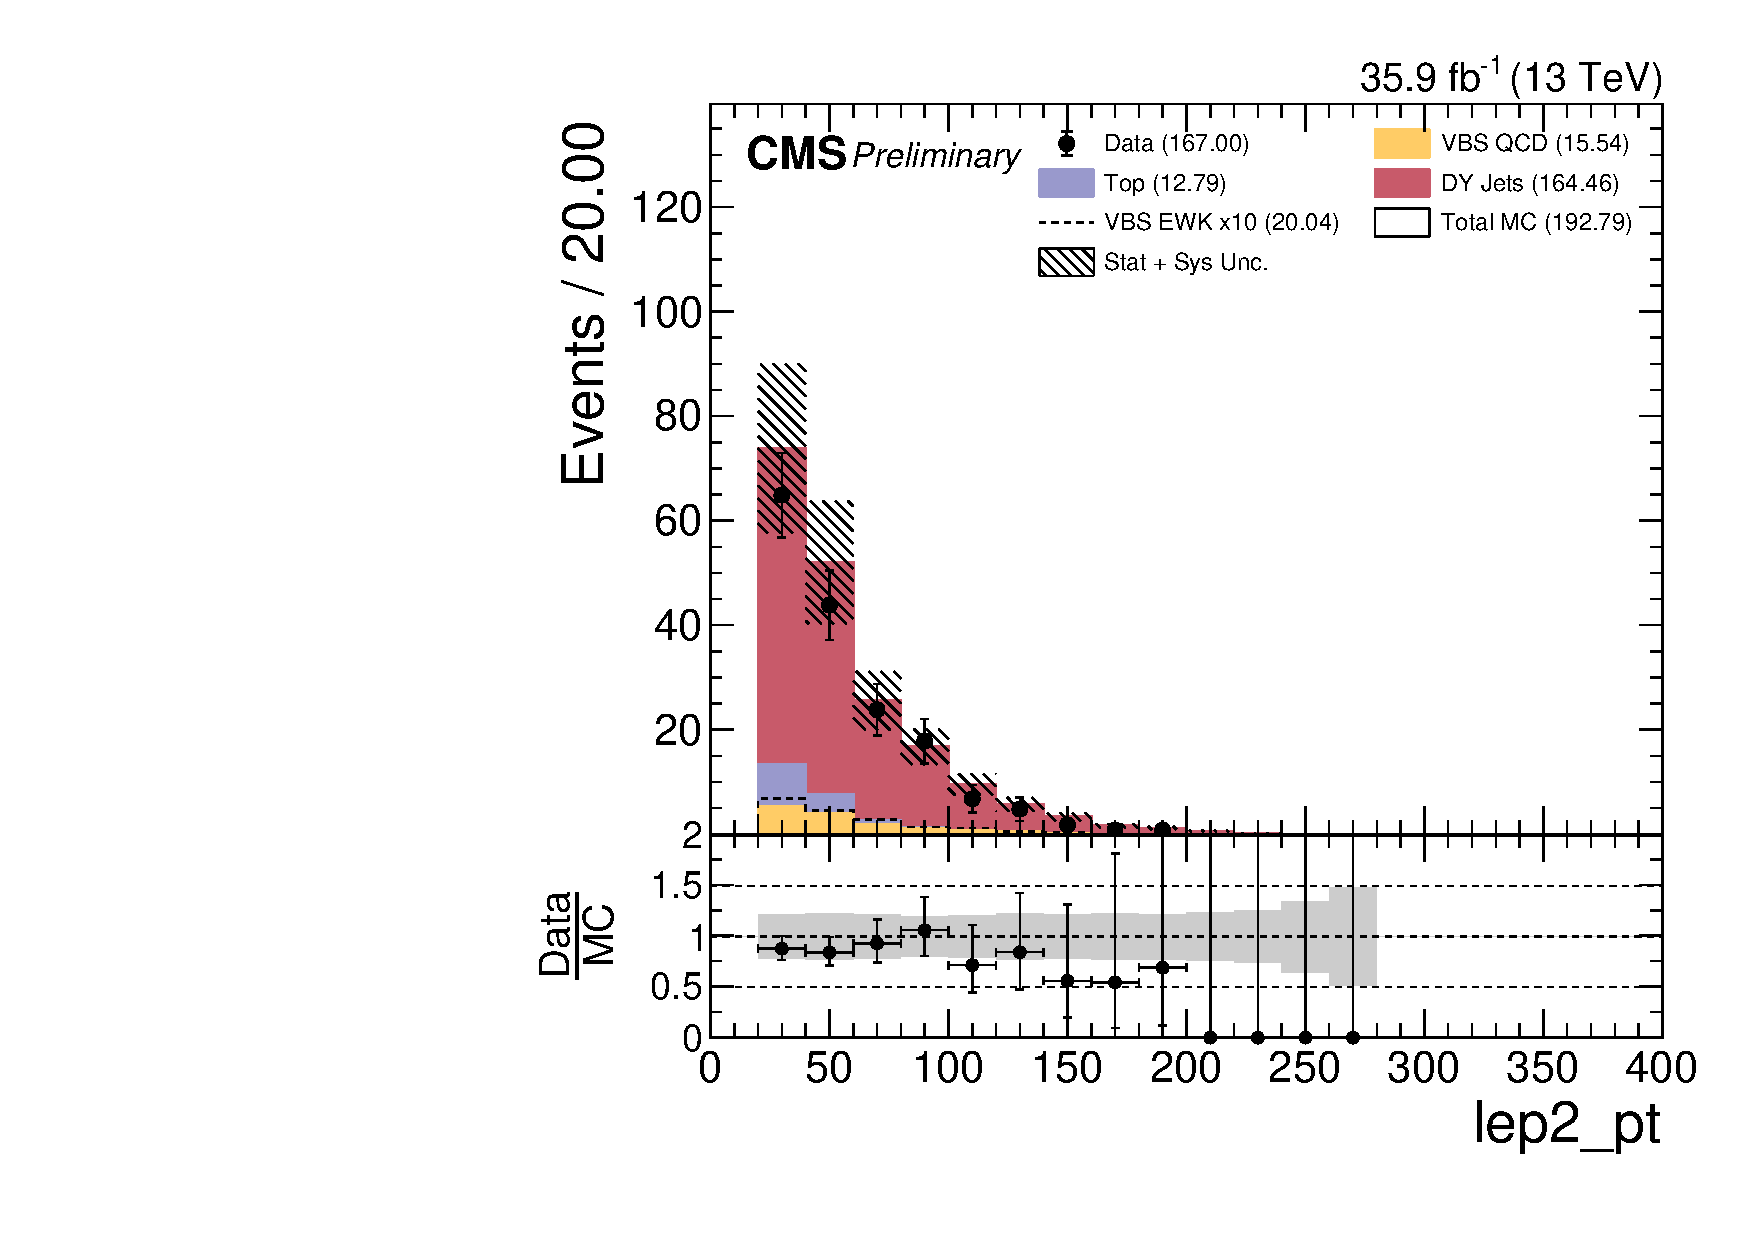
\includegraphics[width=0.335\textwidth]{analysis_plots/2016_zv/cr_vjets_e/lep2_pt.pdf} \hspace{-10pt}
  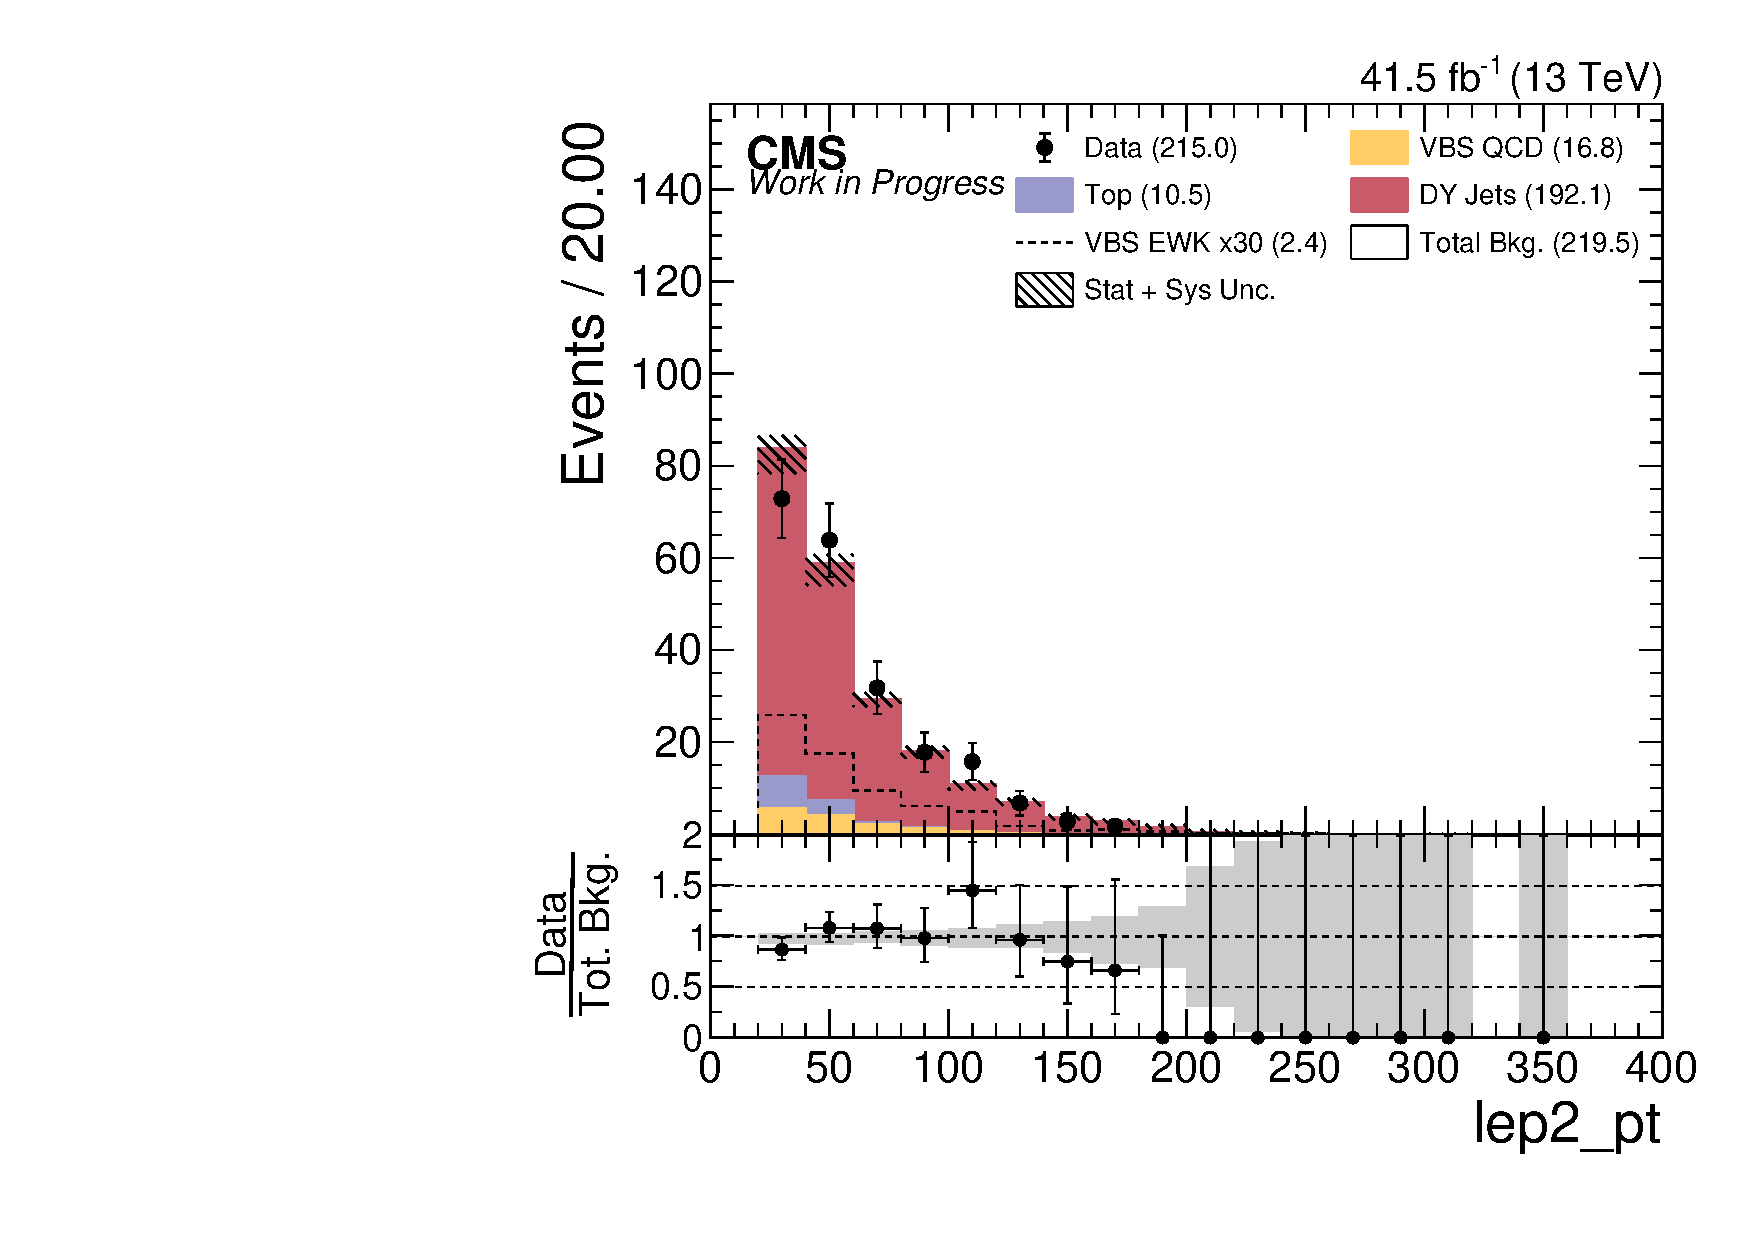
\includegraphics[width=0.335\textwidth]{analysis_plots/2017_zv/cr_vjets_e/lep2_pt.pdf} \hspace{-10pt}
  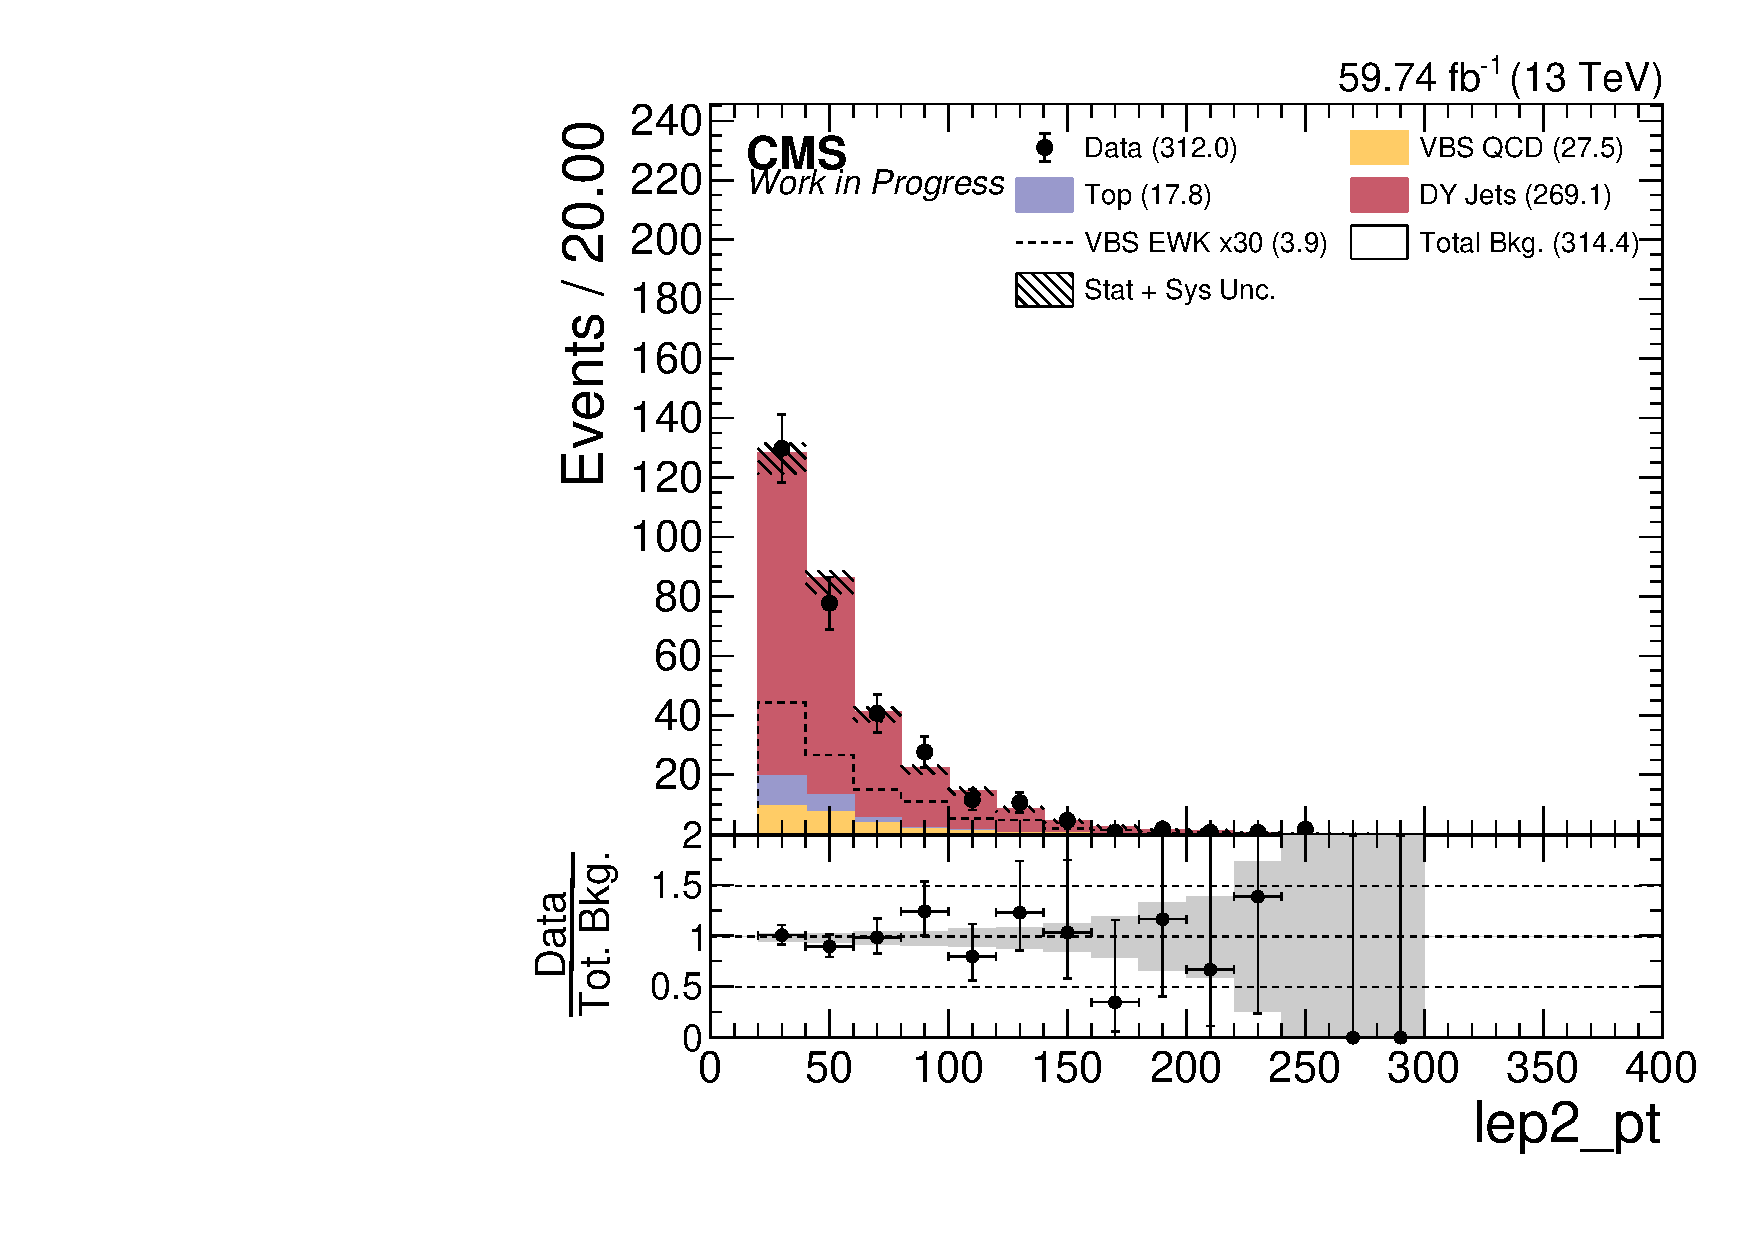
\includegraphics[width=0.335\textwidth]{analysis_plots/2018_zv/cr_vjets_e/lep2_pt.pdf} \hspace{-10pt} \\
  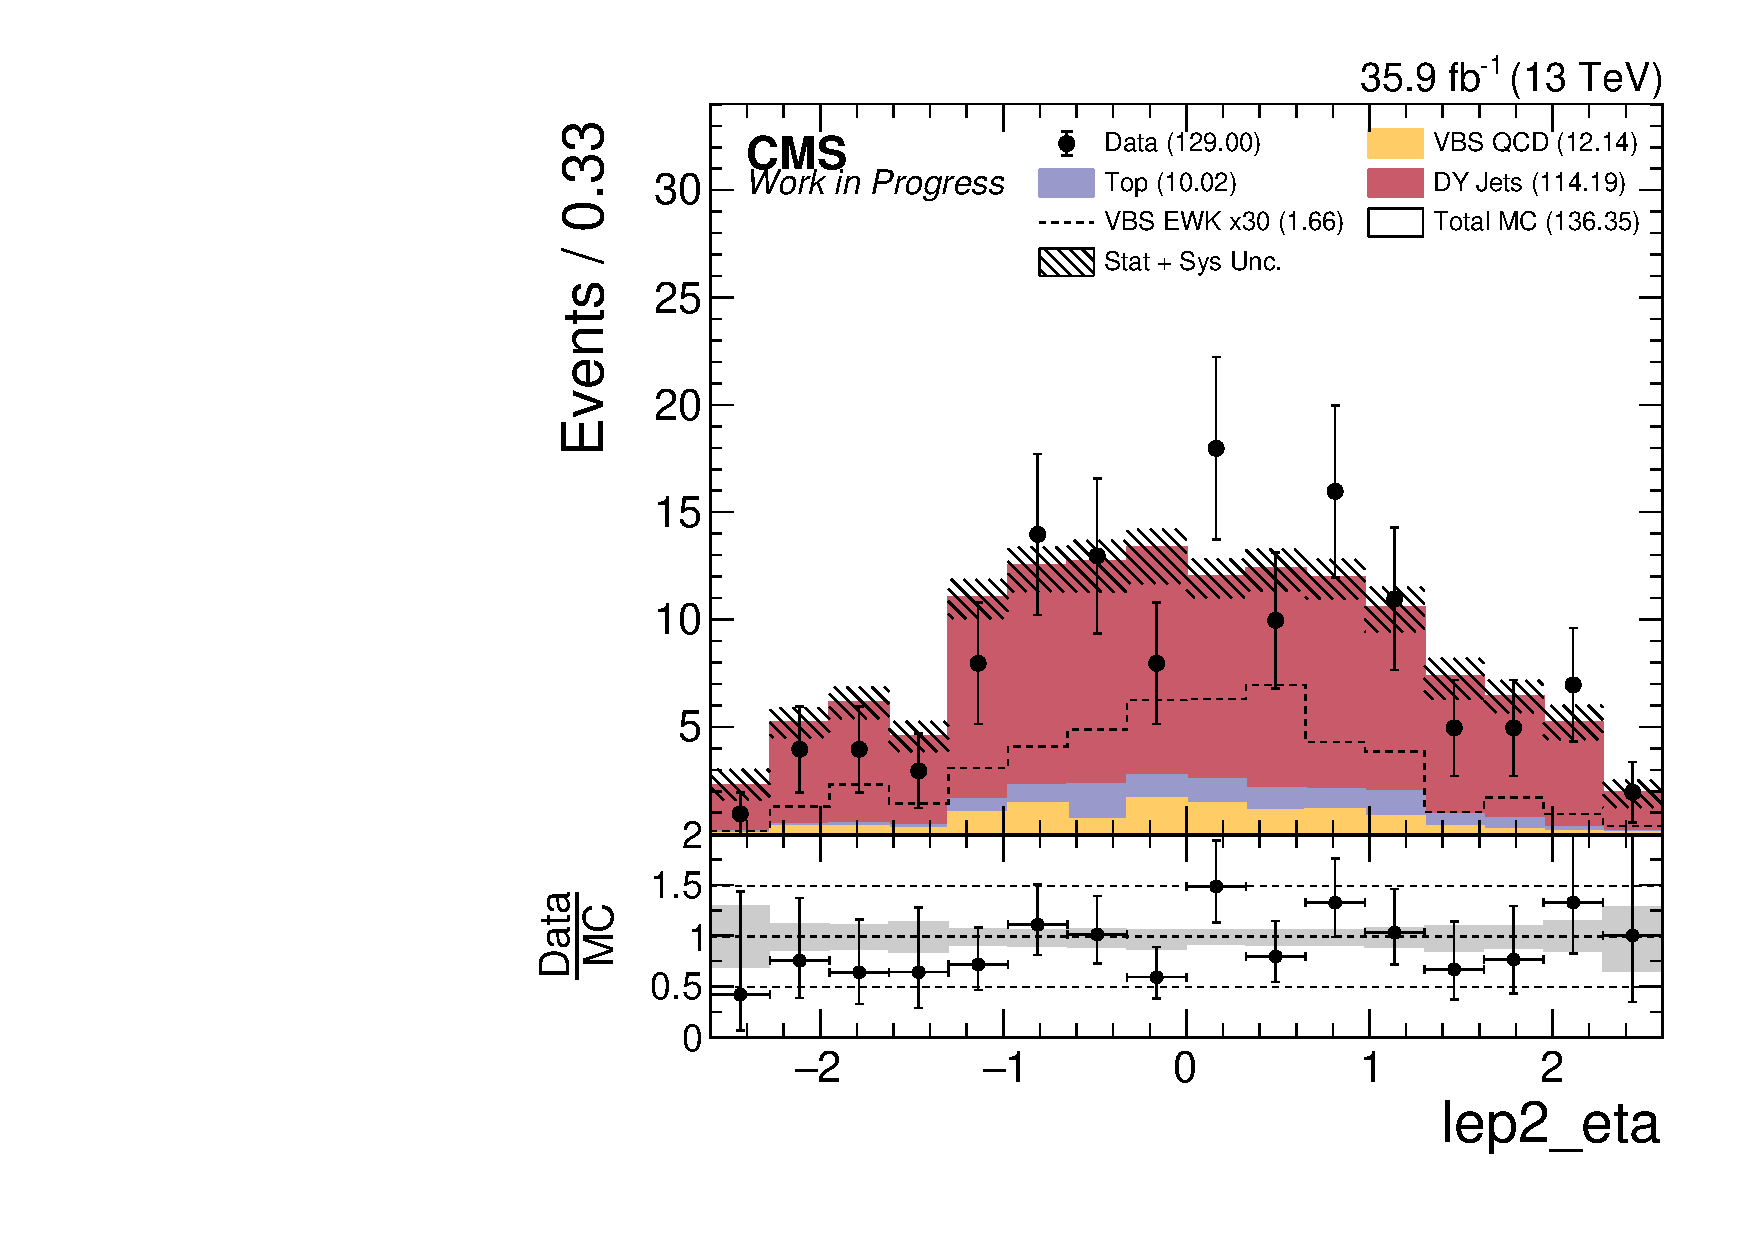
\includegraphics[width=0.335\textwidth]{analysis_plots/2016_zv/cr_vjets_e/lep2_eta.pdf} \hspace{-10pt}
  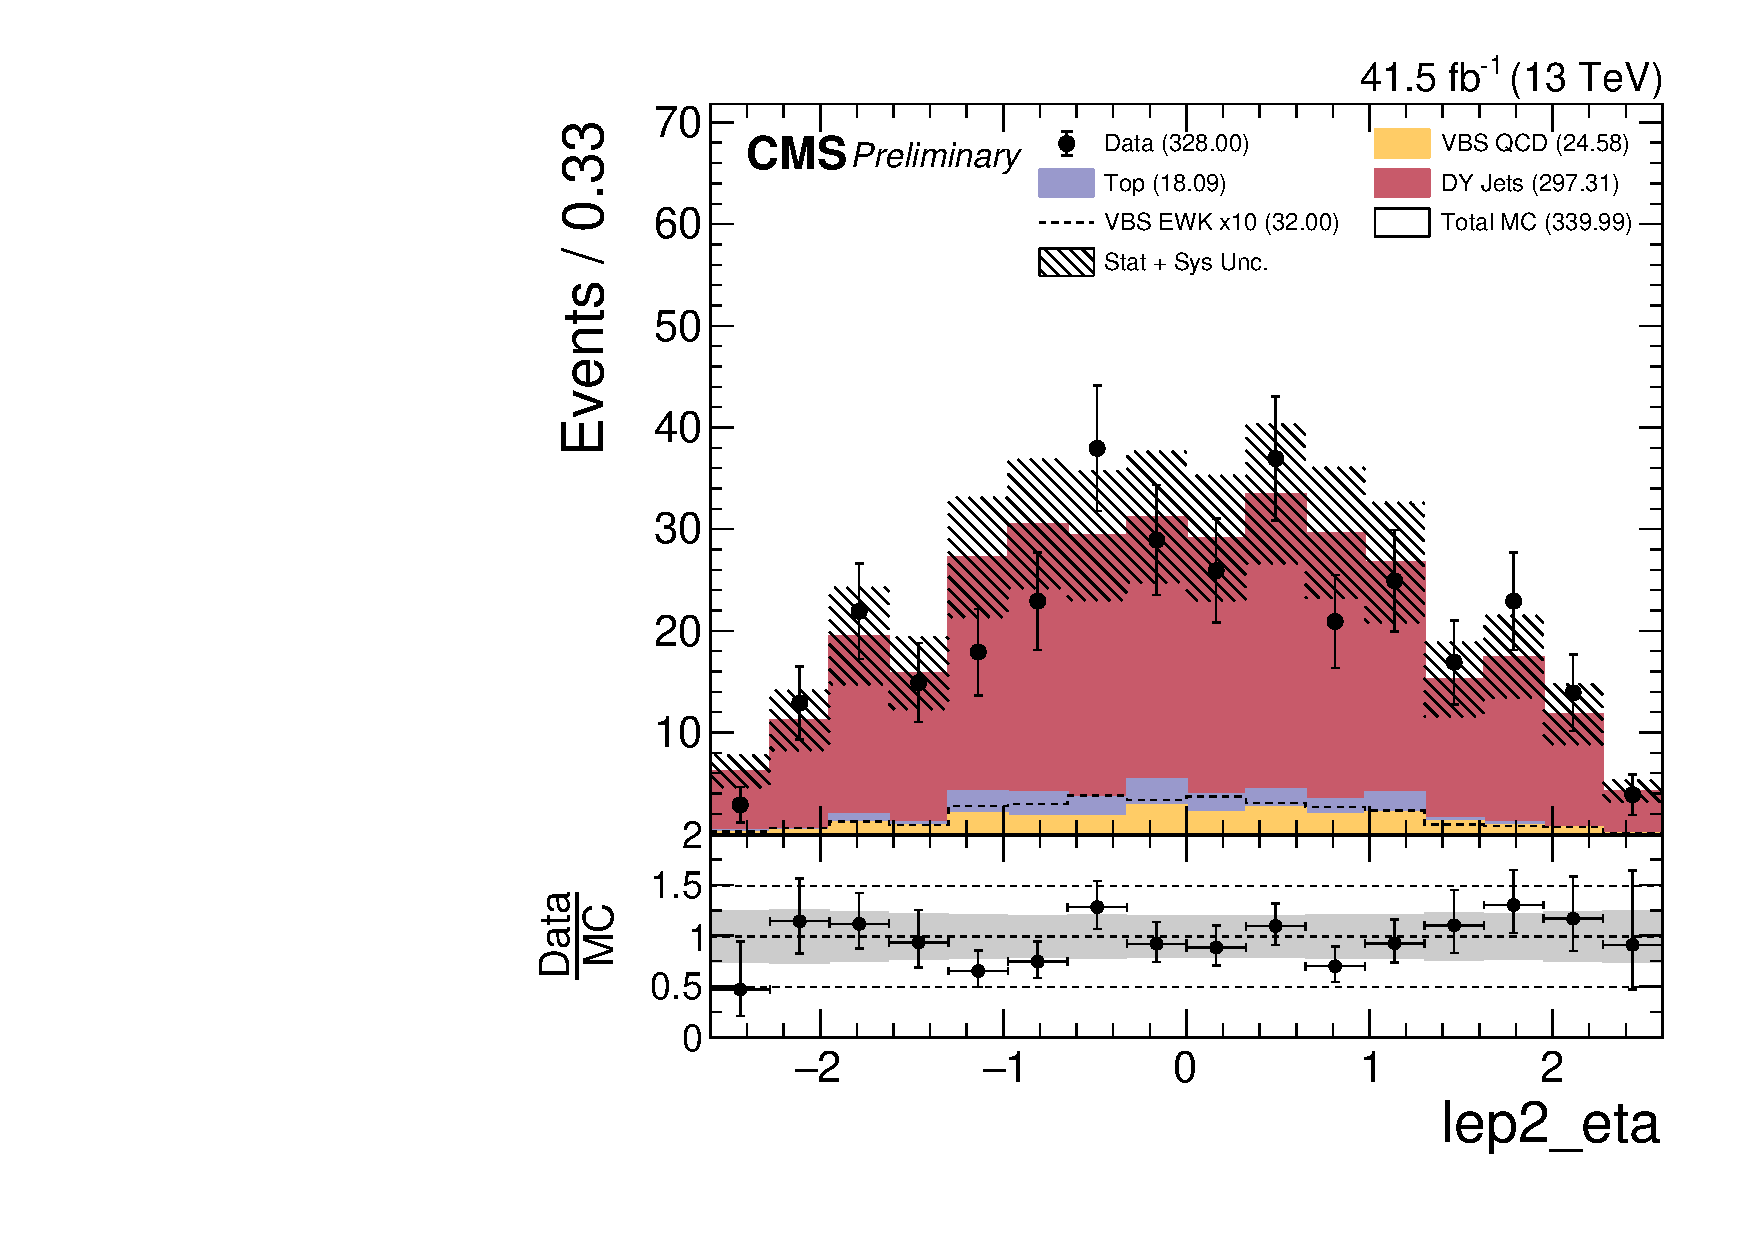
\includegraphics[width=0.335\textwidth]{analysis_plots/2017_zv/cr_vjets_e/lep2_eta.pdf} \hspace{-10pt}
  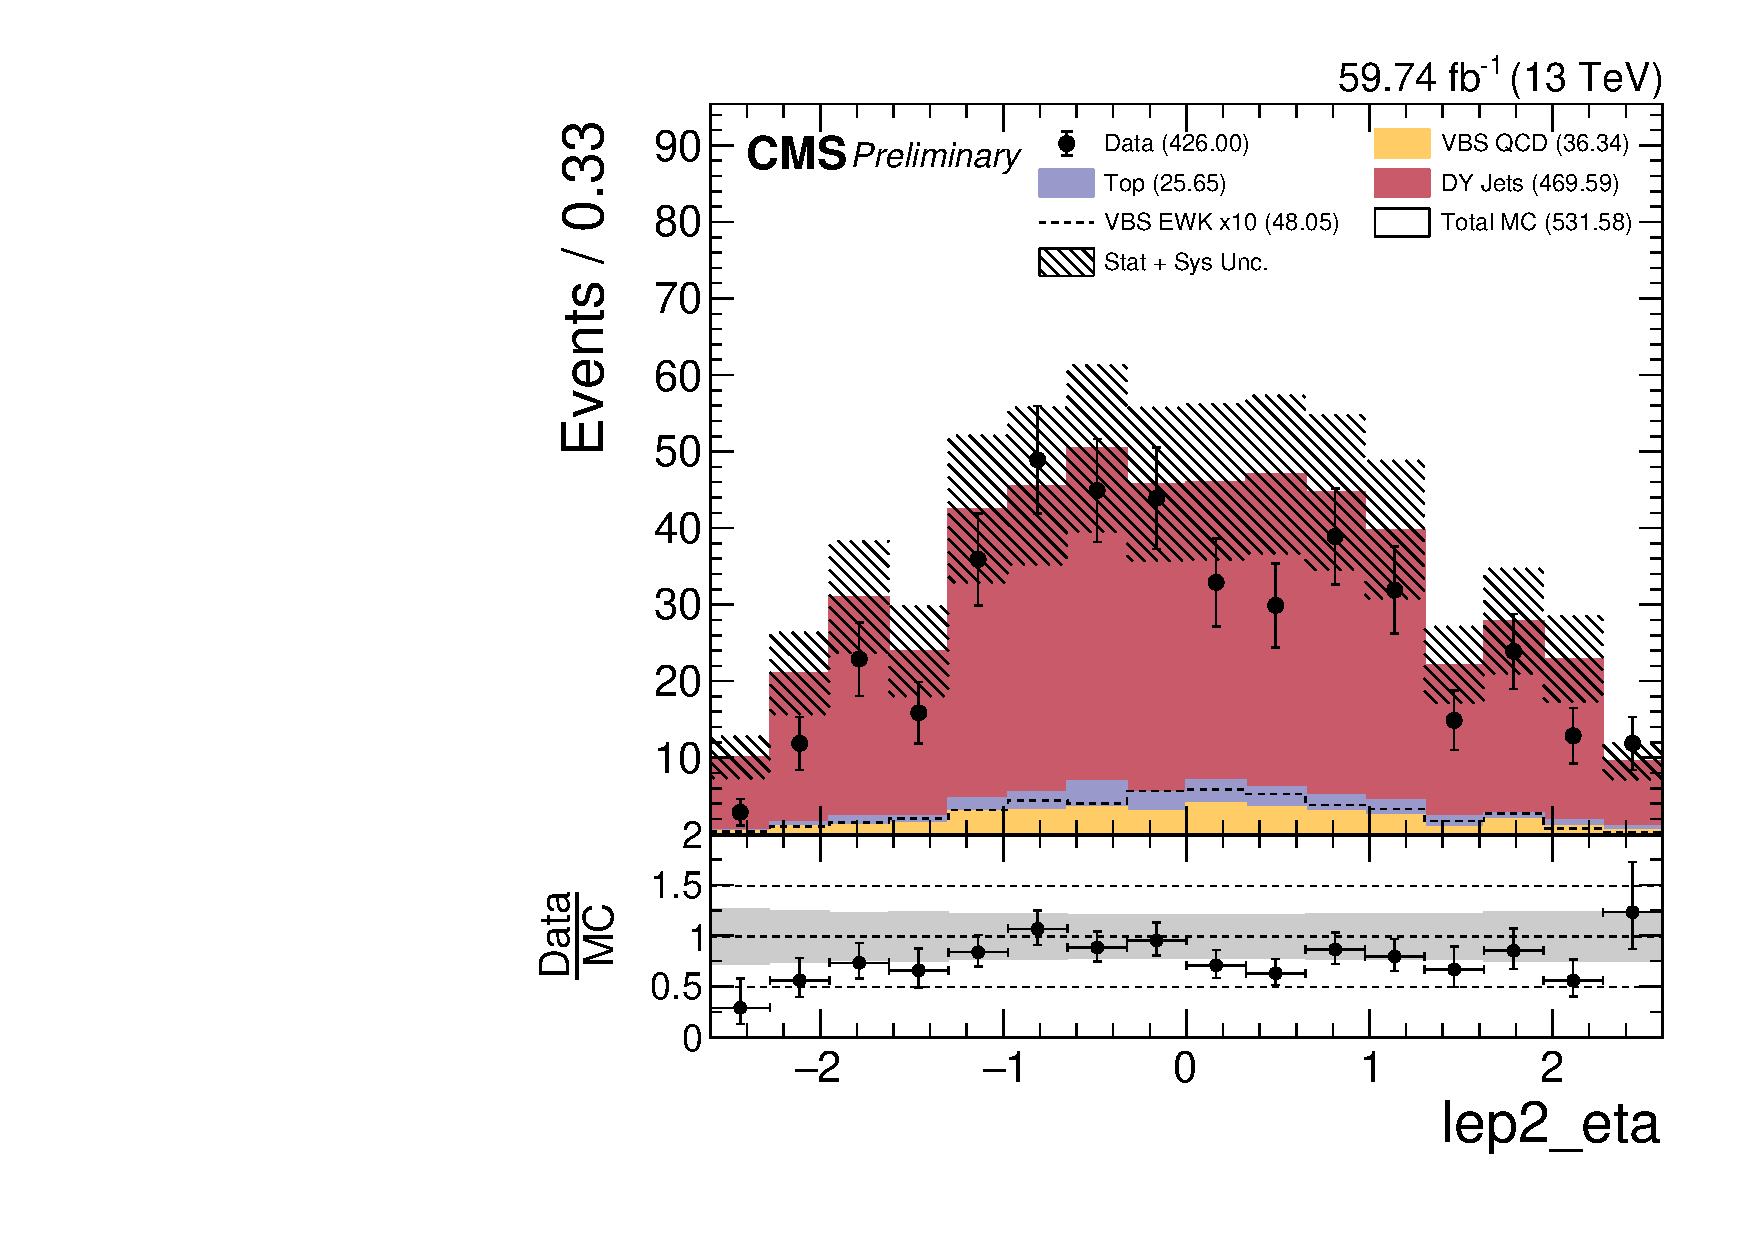
\includegraphics[width=0.335\textwidth]{analysis_plots/2018_zv/cr_vjets_e/lep2_eta.pdf} \hspace{-10pt} \\
  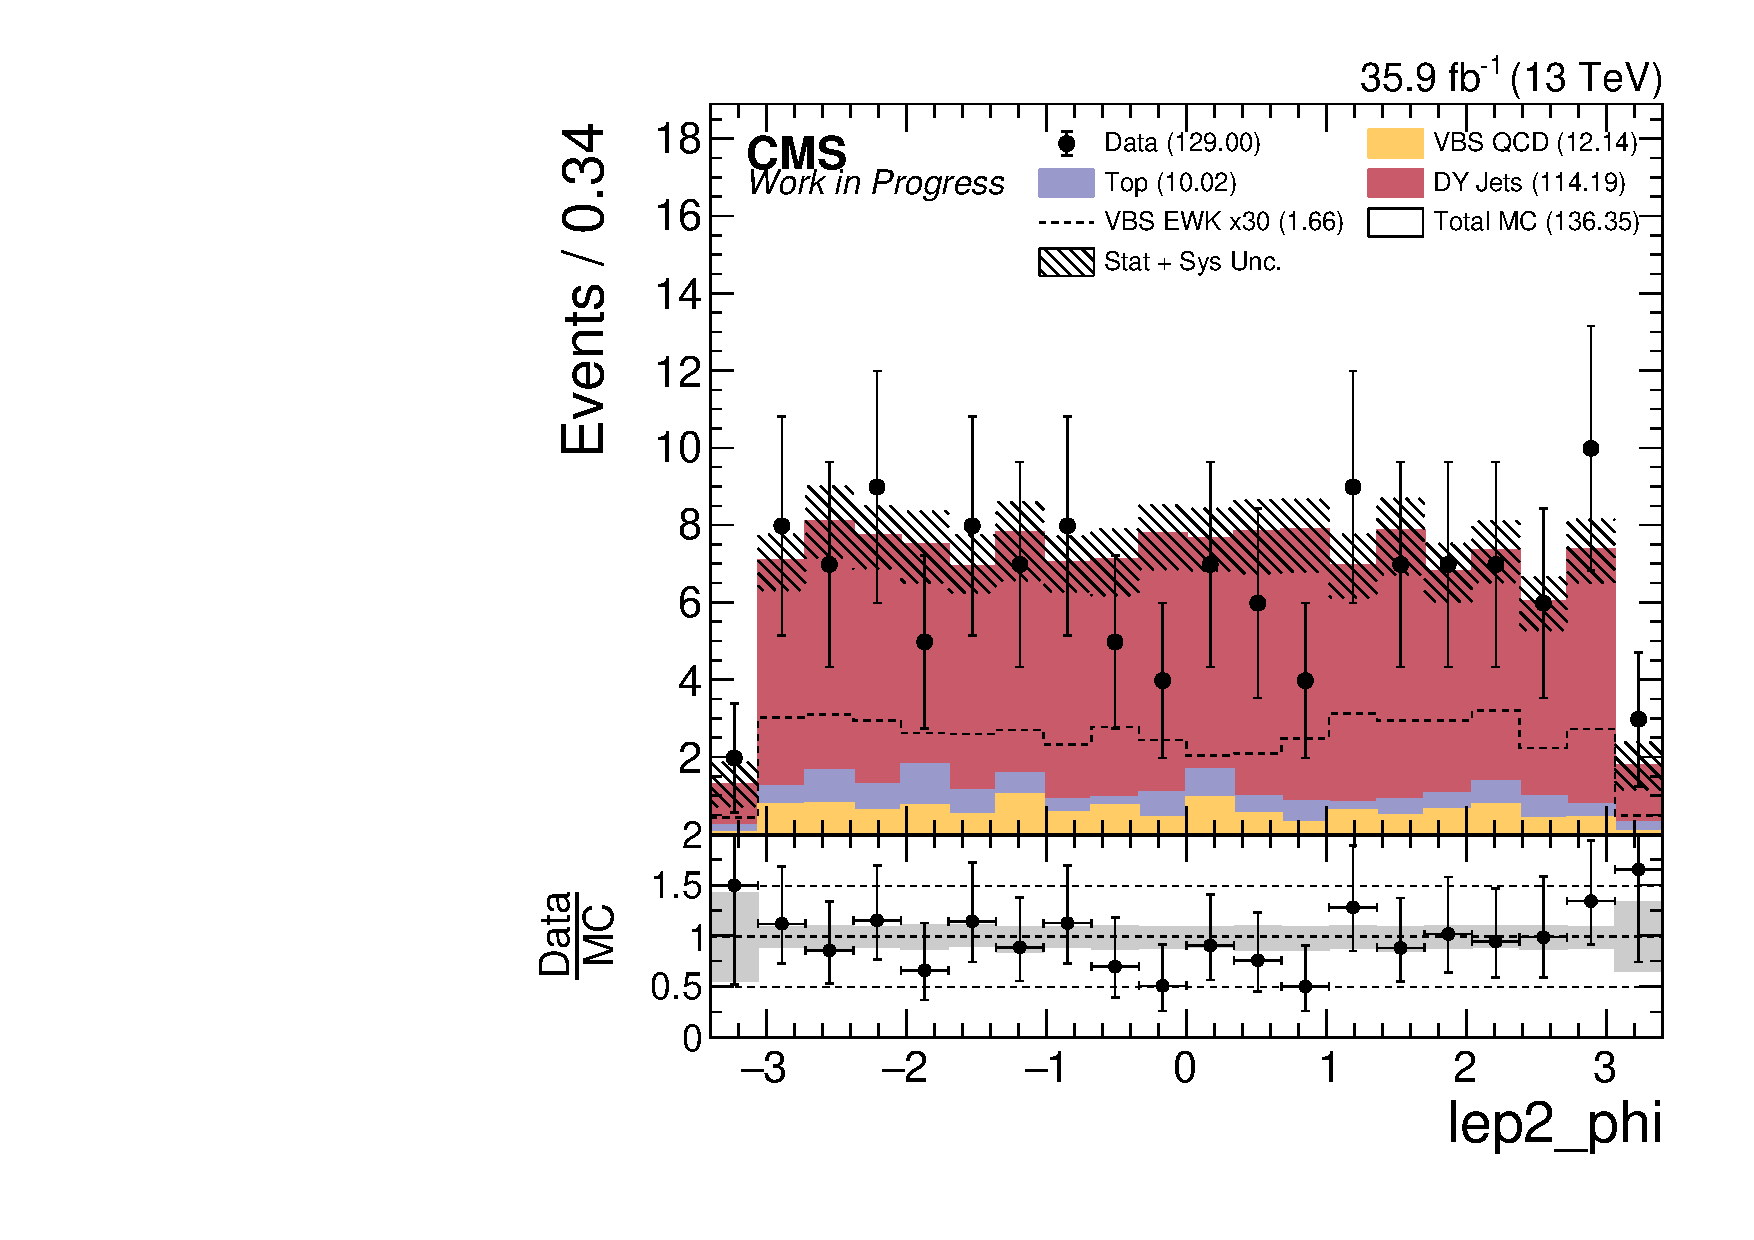
\includegraphics[width=0.335\textwidth]{analysis_plots/2016_zv/cr_vjets_e/lep2_phi.pdf} \hspace{-10pt}
  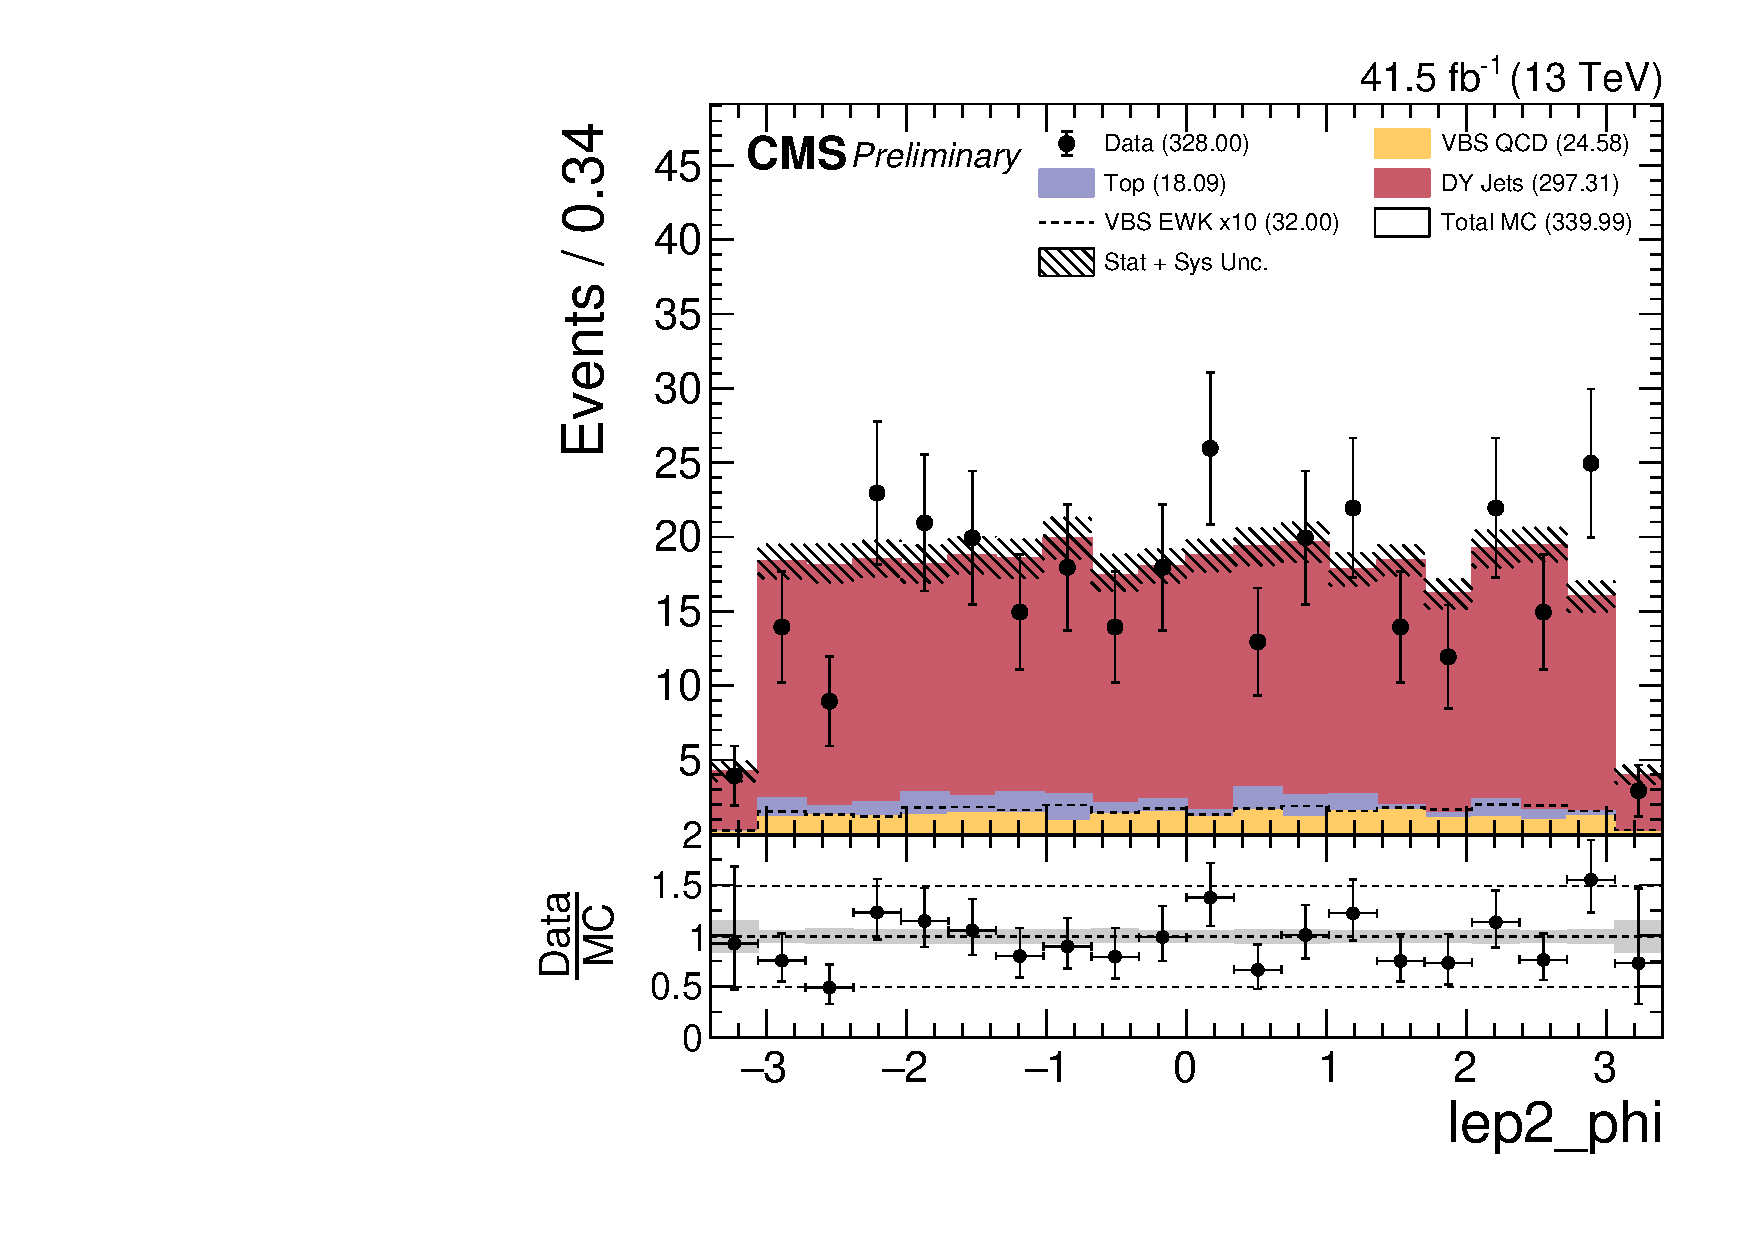
\includegraphics[width=0.335\textwidth]{analysis_plots/2017_zv/cr_vjets_e/lep2_phi.pdf} \hspace{-10pt}
  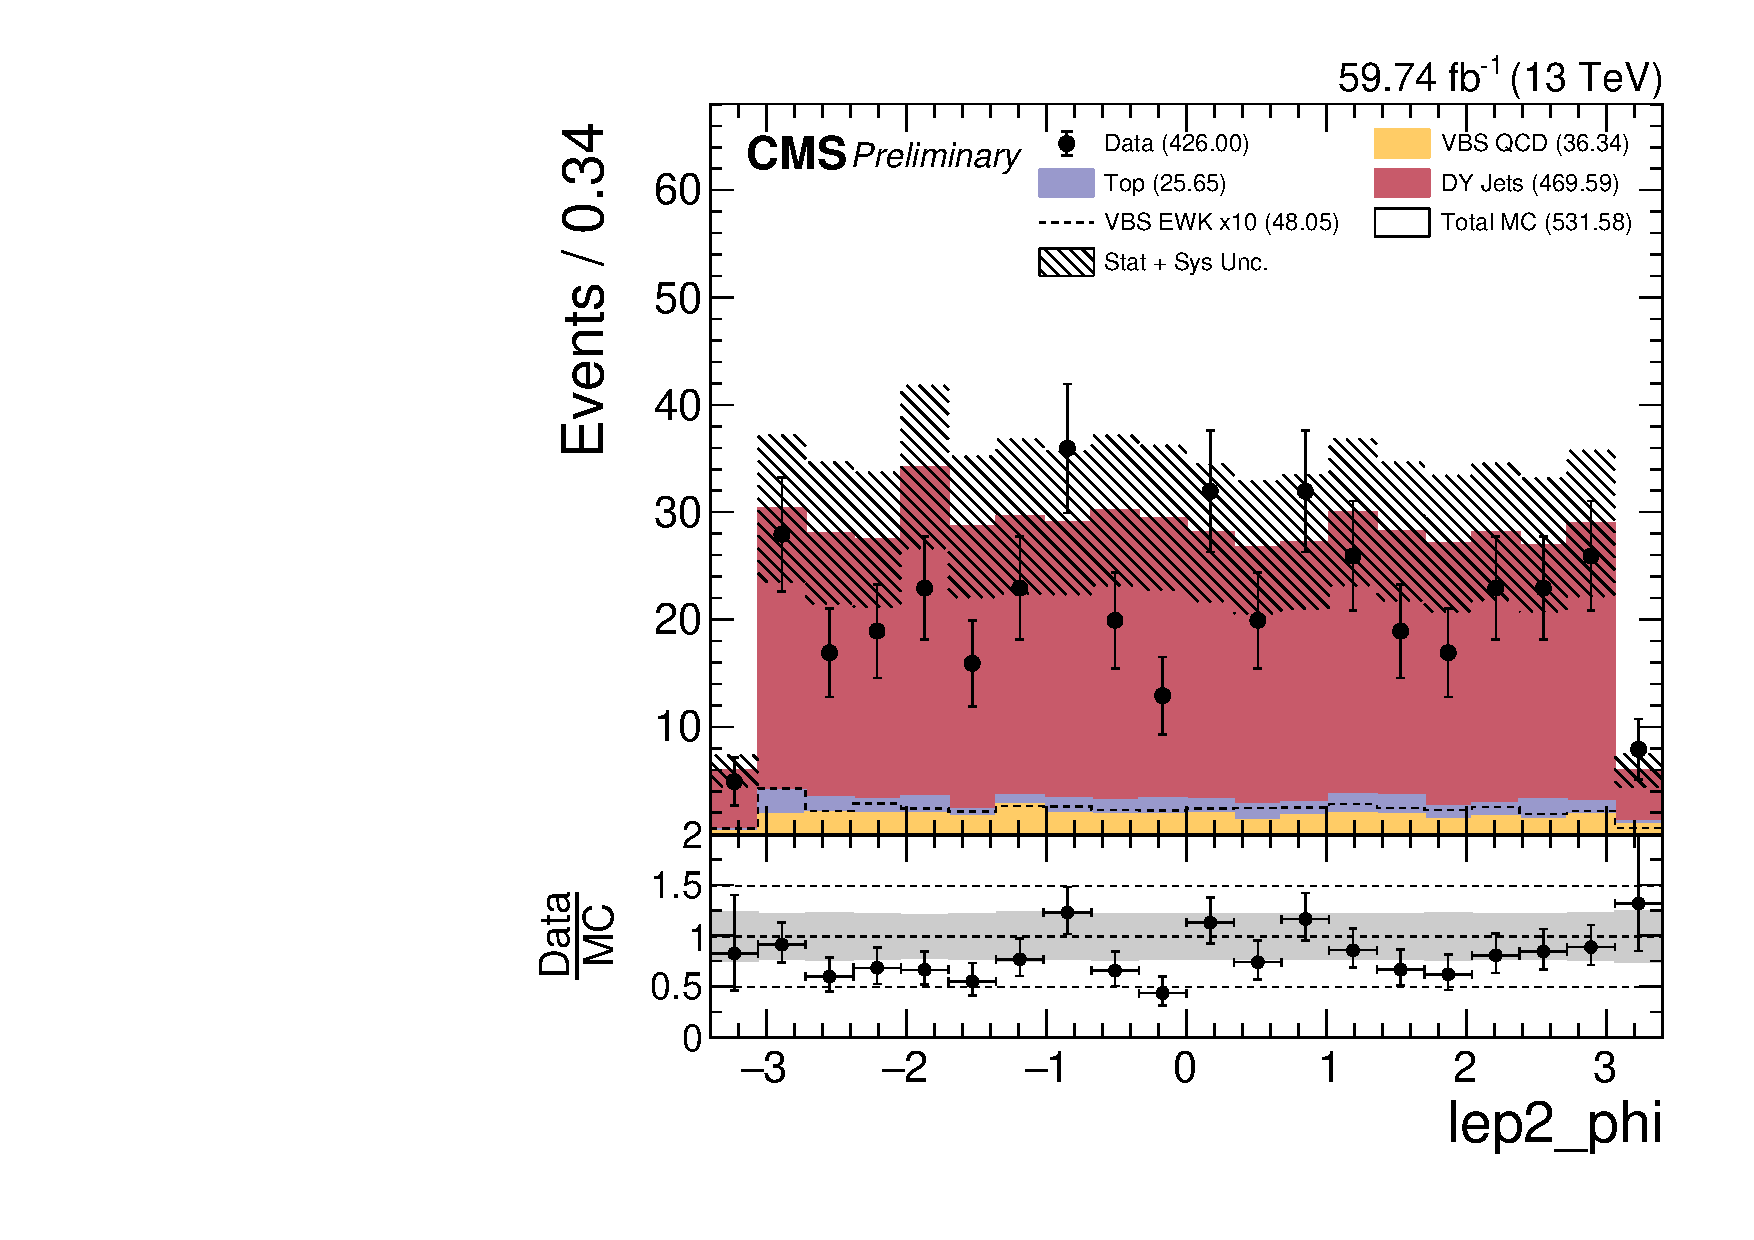
\includegraphics[width=0.335\textwidth]{analysis_plots/2018_zv/cr_vjets_e/lep2_phi.pdf} \hspace{-10pt} \\
  \caption[DY+Jets Control Region: Trailing electron kinematics in Boosted ZV Channel]%
  {DY+Jets Control Region: Trailing electron kinematics in Boosted ZV Channel.
    Error bars include statistical uncertainty on total background,
    JES and QCD scale systematic on DY+Jets and VBS\_QCD MC\@. From Left to Right: 2016,
    2017, and 2018. From Top to Bottom: \( p_T \), \( \eta \), and \( \phi \).}%
  \label{fig:zv-cr-vjets-e-lep2-pt-eta-phi}
\end{figure}

\begin{figure}[!ht]
  \centering
  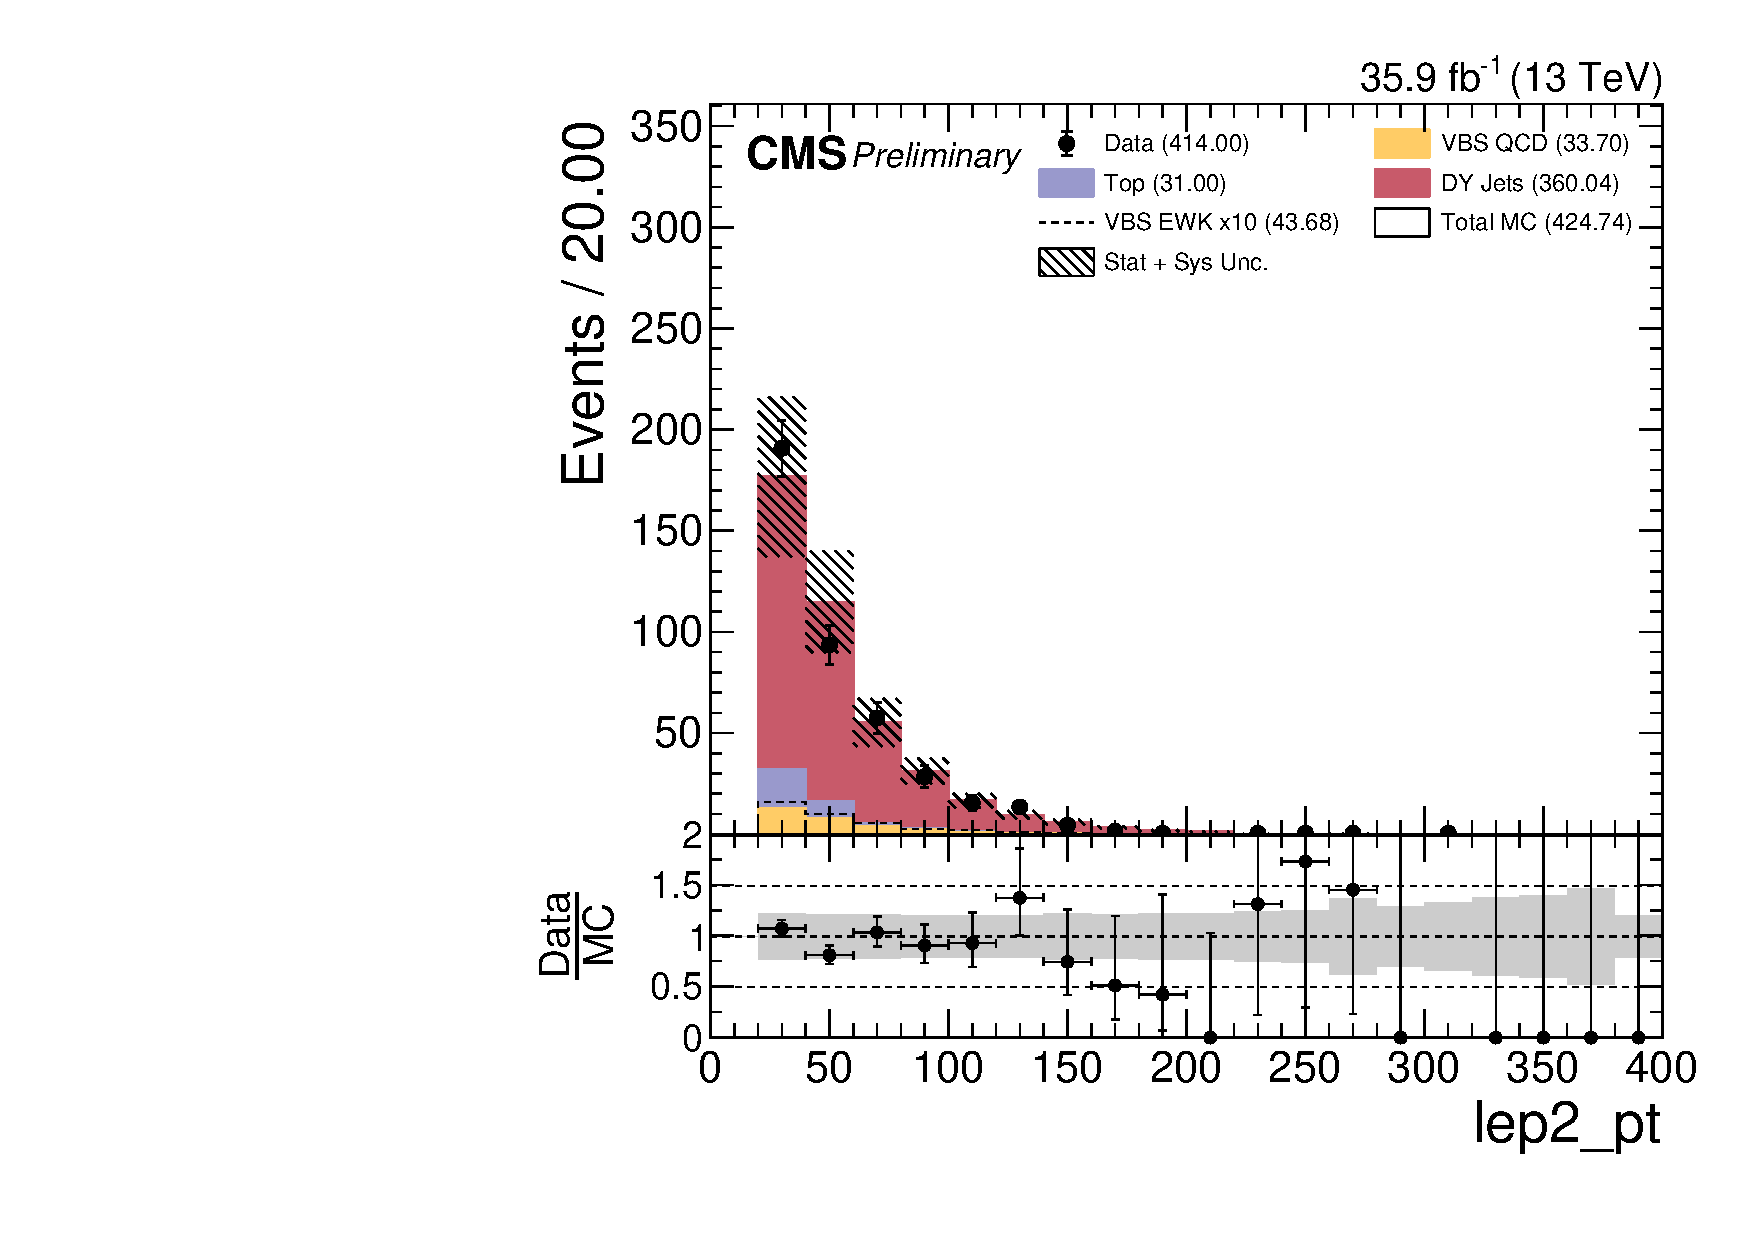
\includegraphics[width=0.335\textwidth]{analysis_plots/2016_zv/cr_vjets_m/lep2_pt.pdf} \hspace{-10pt}
  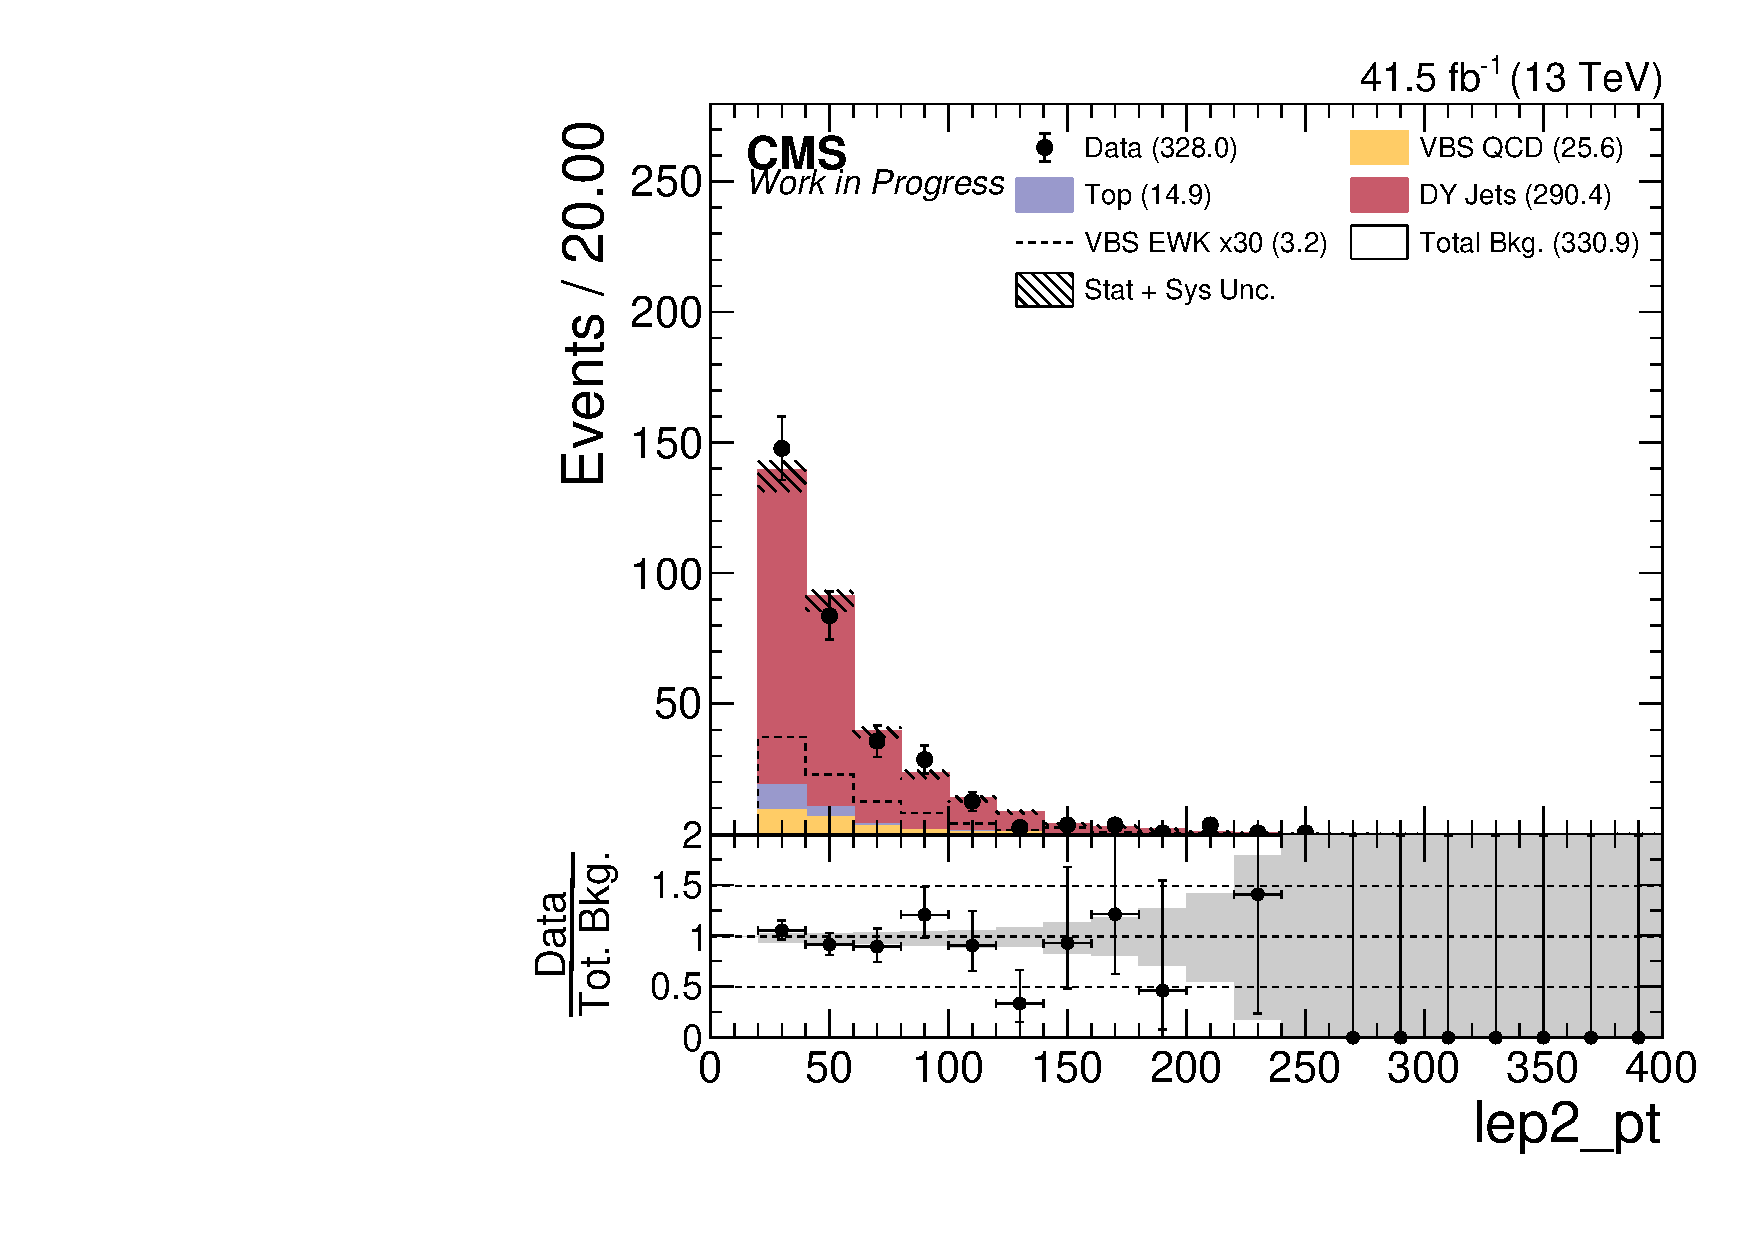
\includegraphics[width=0.335\textwidth]{analysis_plots/2017_zv/cr_vjets_m/lep2_pt.pdf} \hspace{-10pt}
  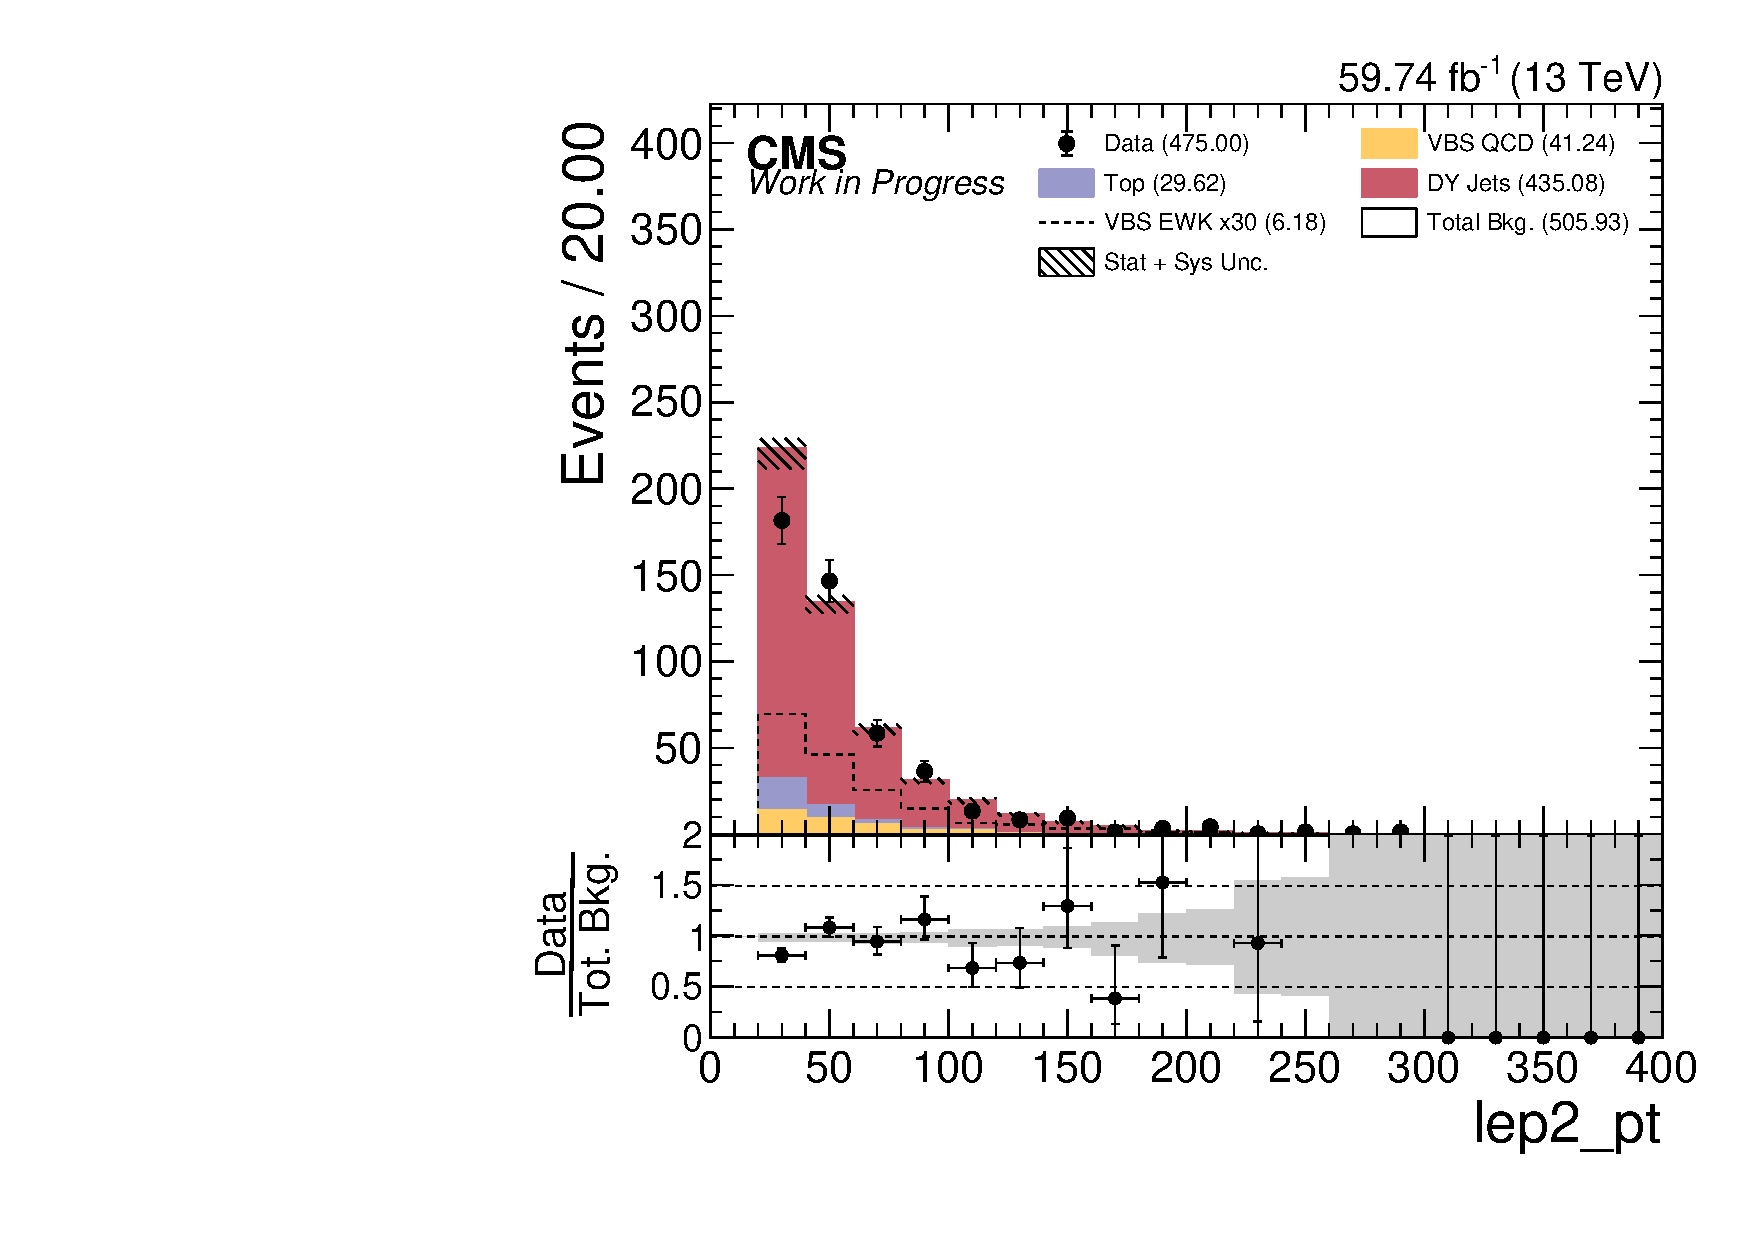
\includegraphics[width=0.335\textwidth]{analysis_plots/2018_zv/cr_vjets_m/lep2_pt.pdf} \hspace{-10pt} \\
  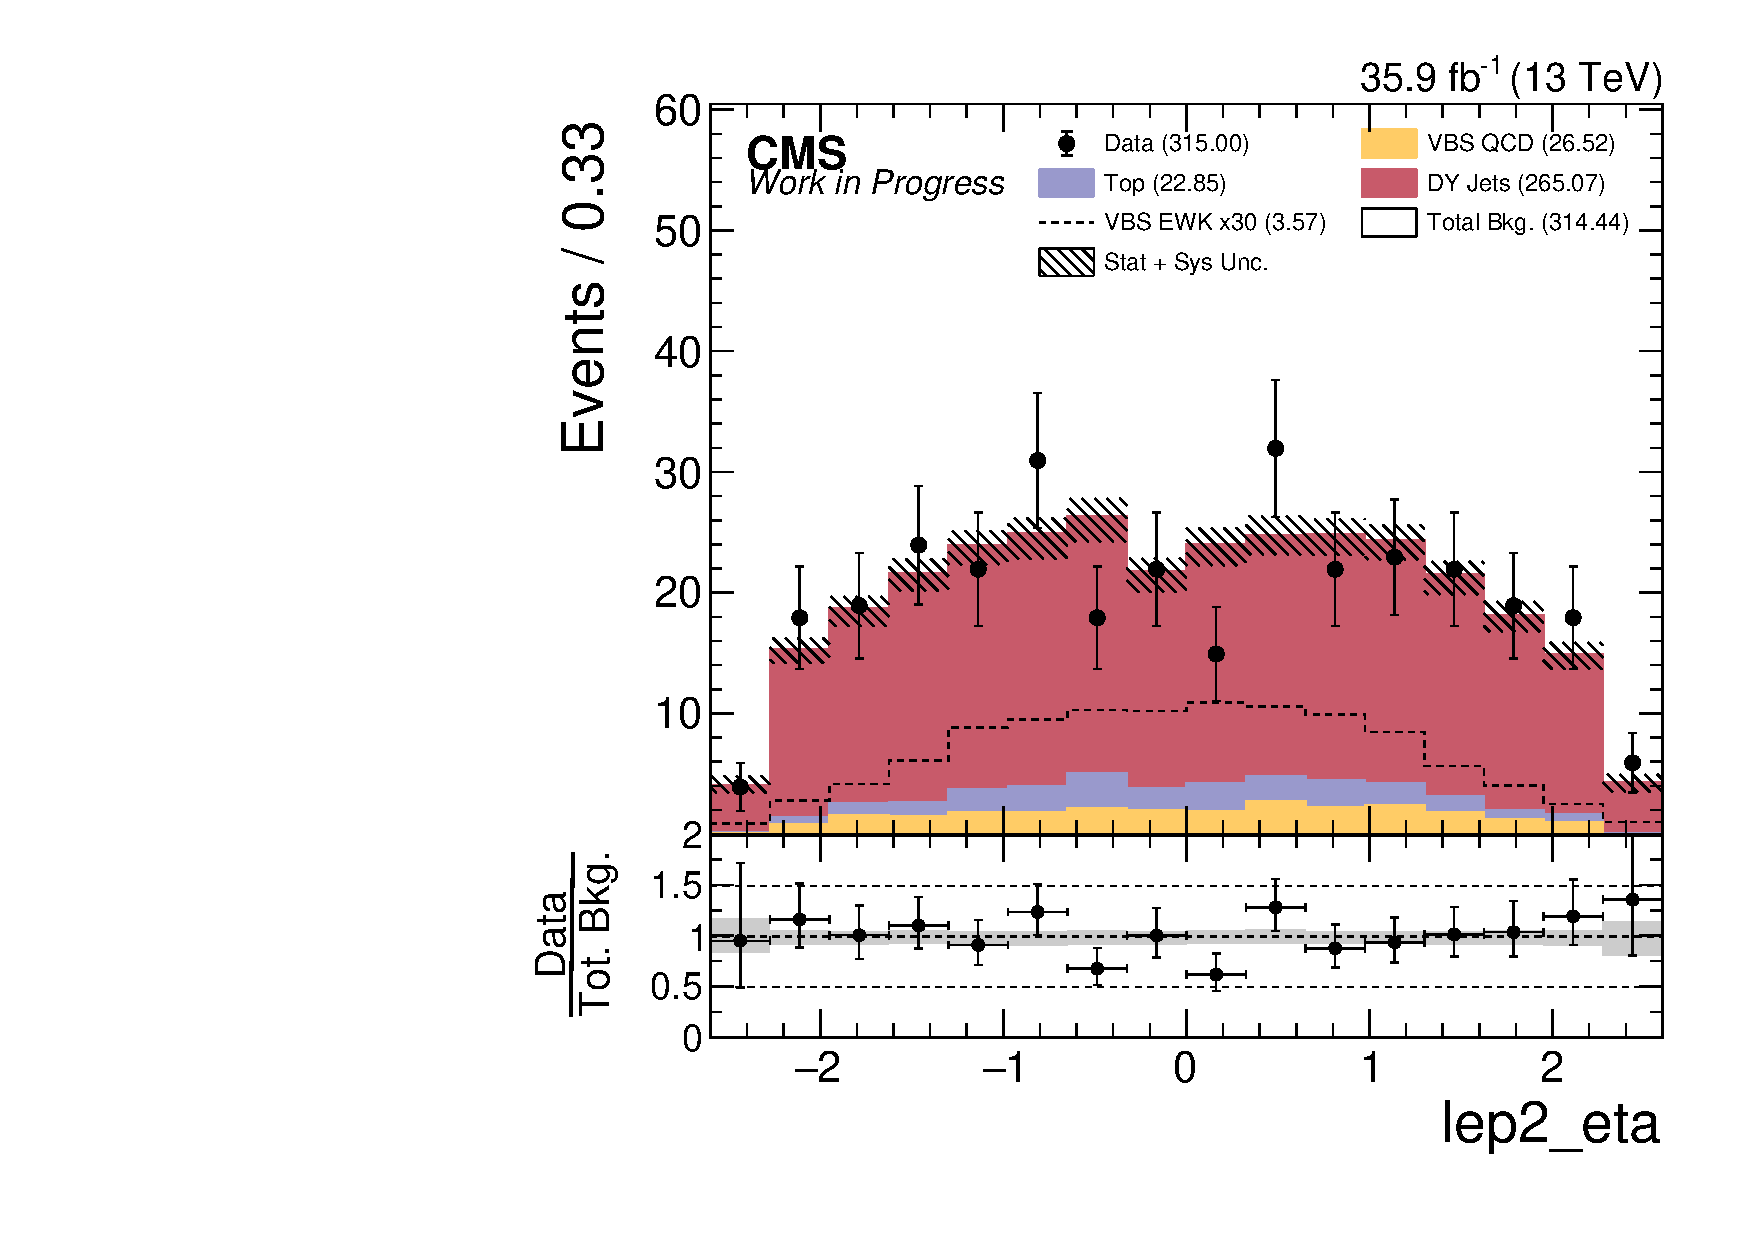
\includegraphics[width=0.335\textwidth]{analysis_plots/2016_zv/cr_vjets_m/lep2_eta.pdf} \hspace{-10pt}
  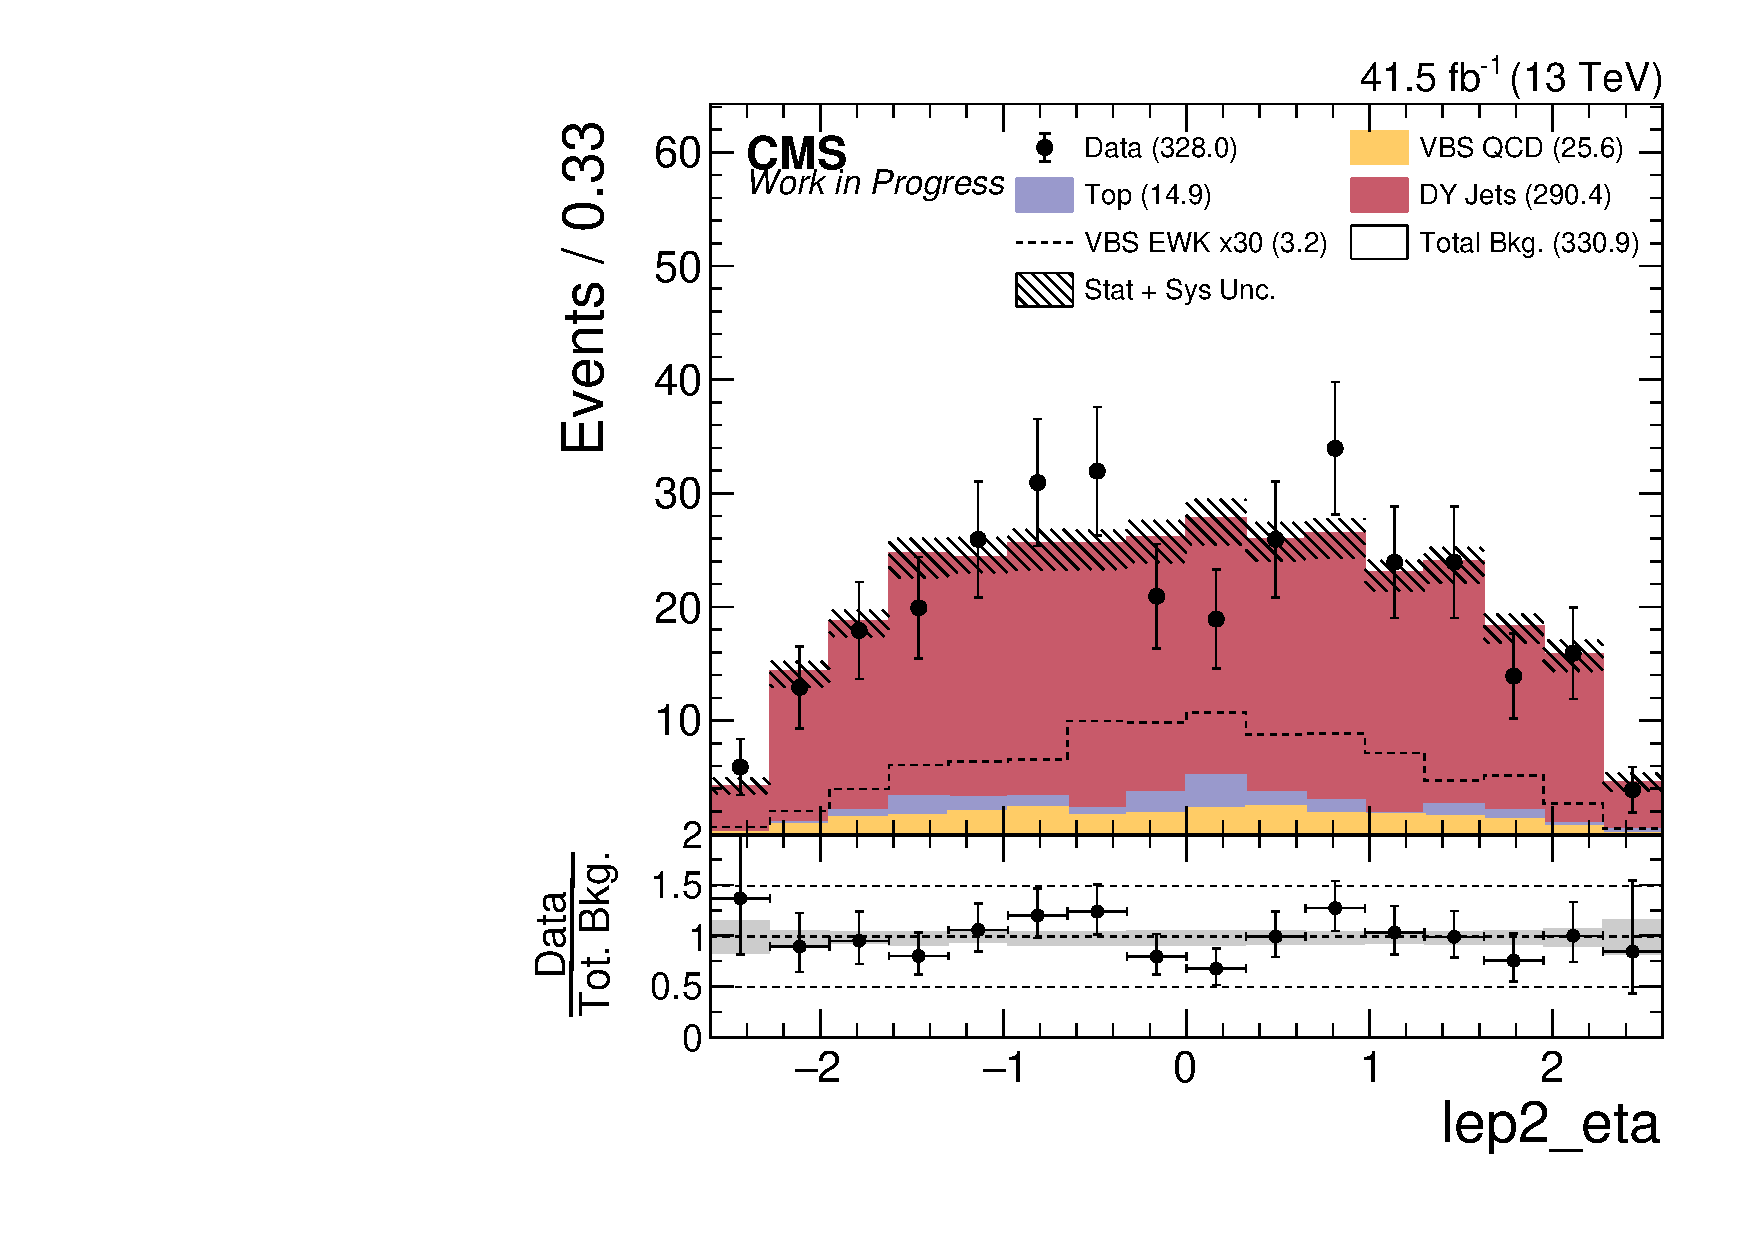
\includegraphics[width=0.335\textwidth]{analysis_plots/2017_zv/cr_vjets_m/lep2_eta.pdf} \hspace{-10pt}
  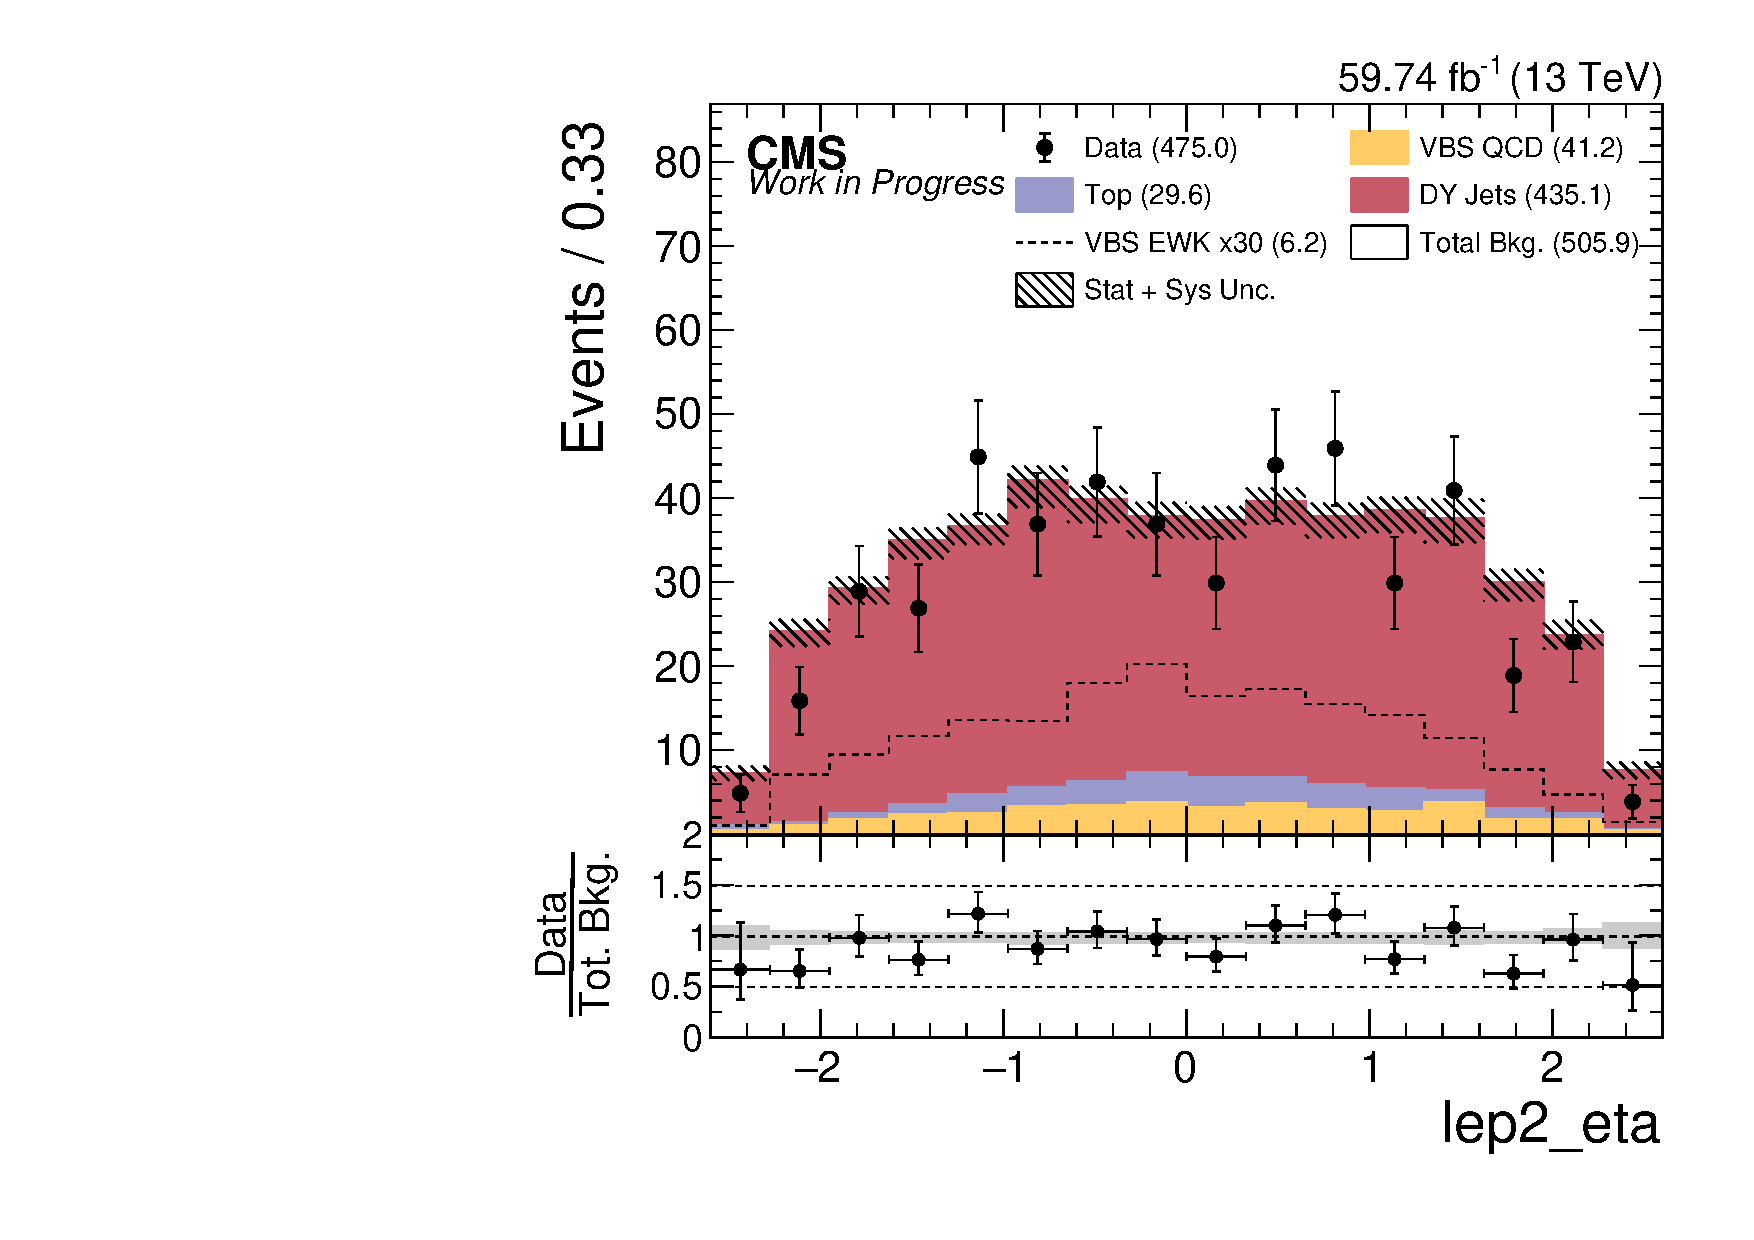
\includegraphics[width=0.335\textwidth]{analysis_plots/2018_zv/cr_vjets_m/lep2_eta.pdf} \hspace{-10pt} \\
  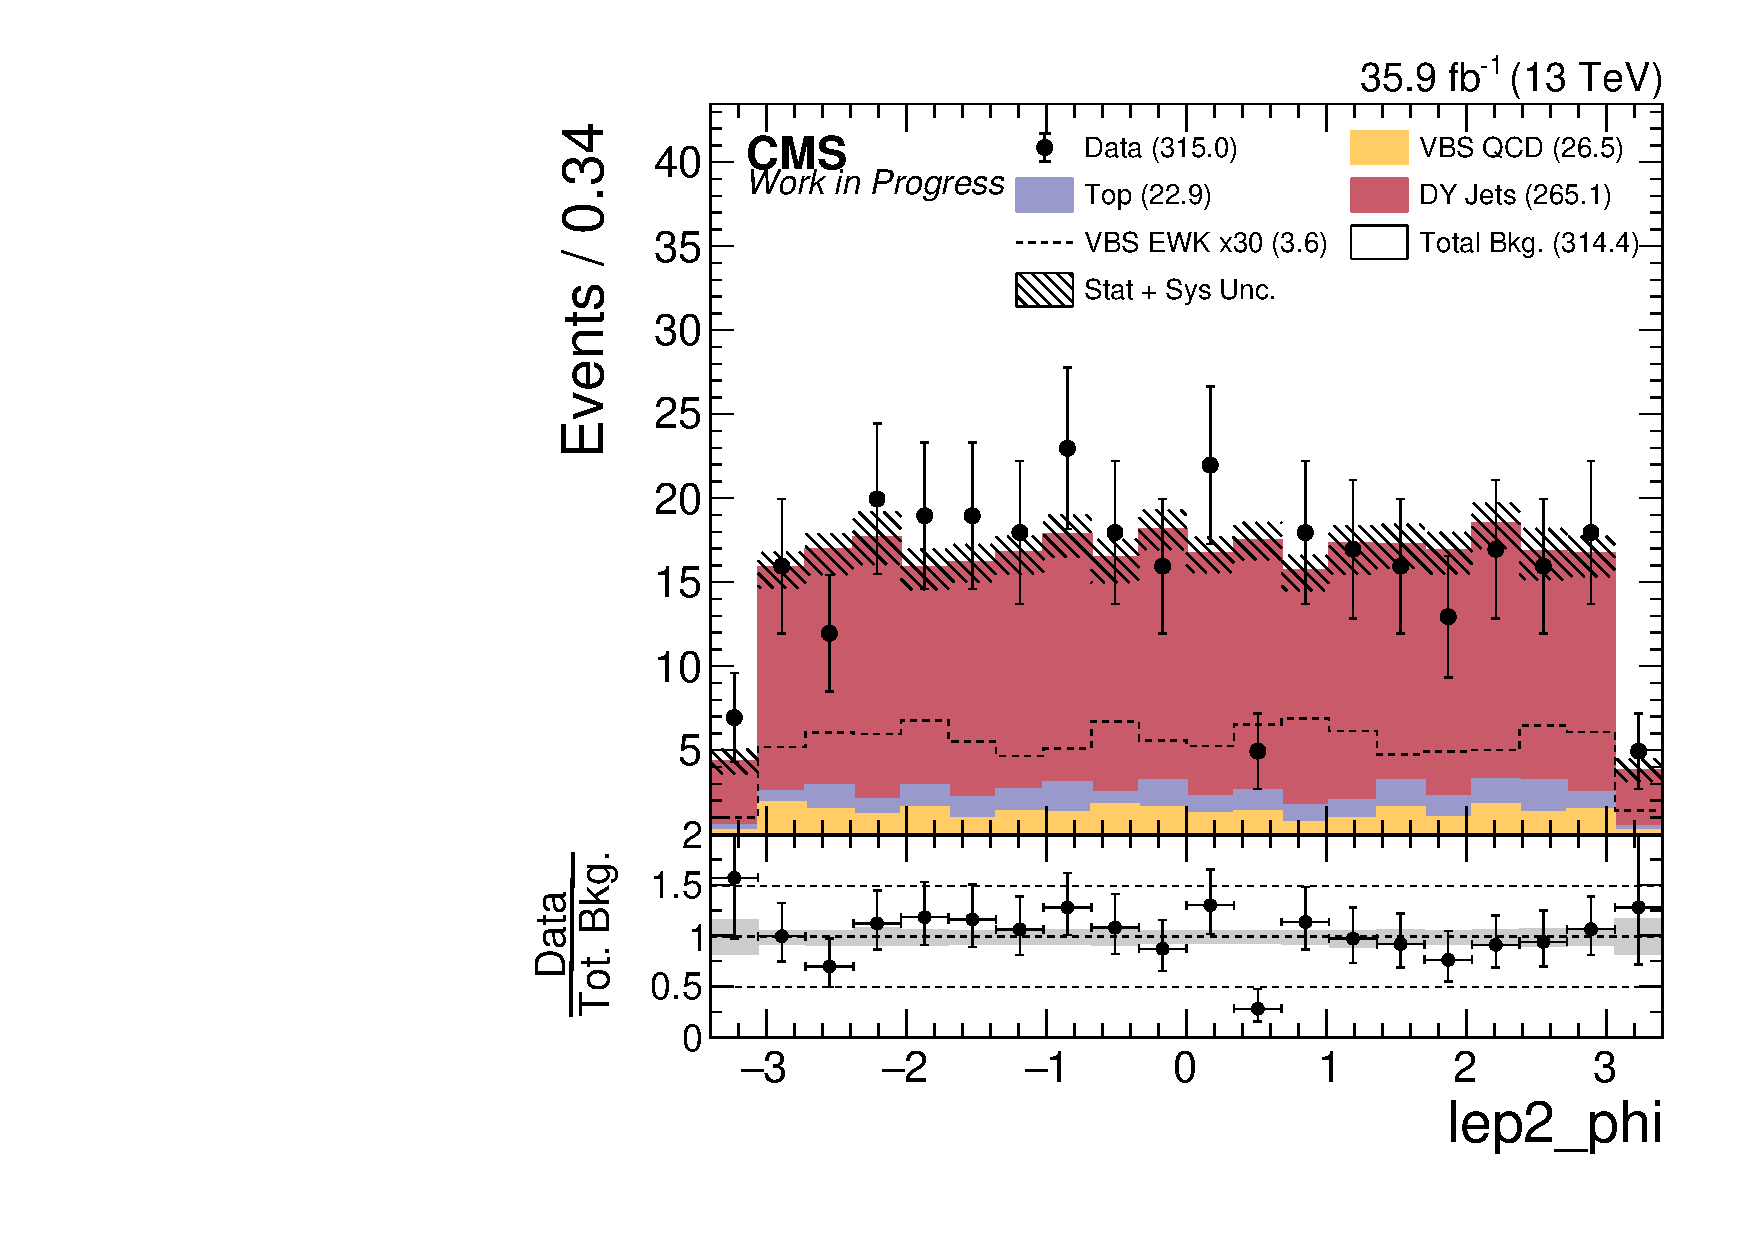
\includegraphics[width=0.335\textwidth]{analysis_plots/2016_zv/cr_vjets_m/lep2_phi.pdf} \hspace{-10pt}
  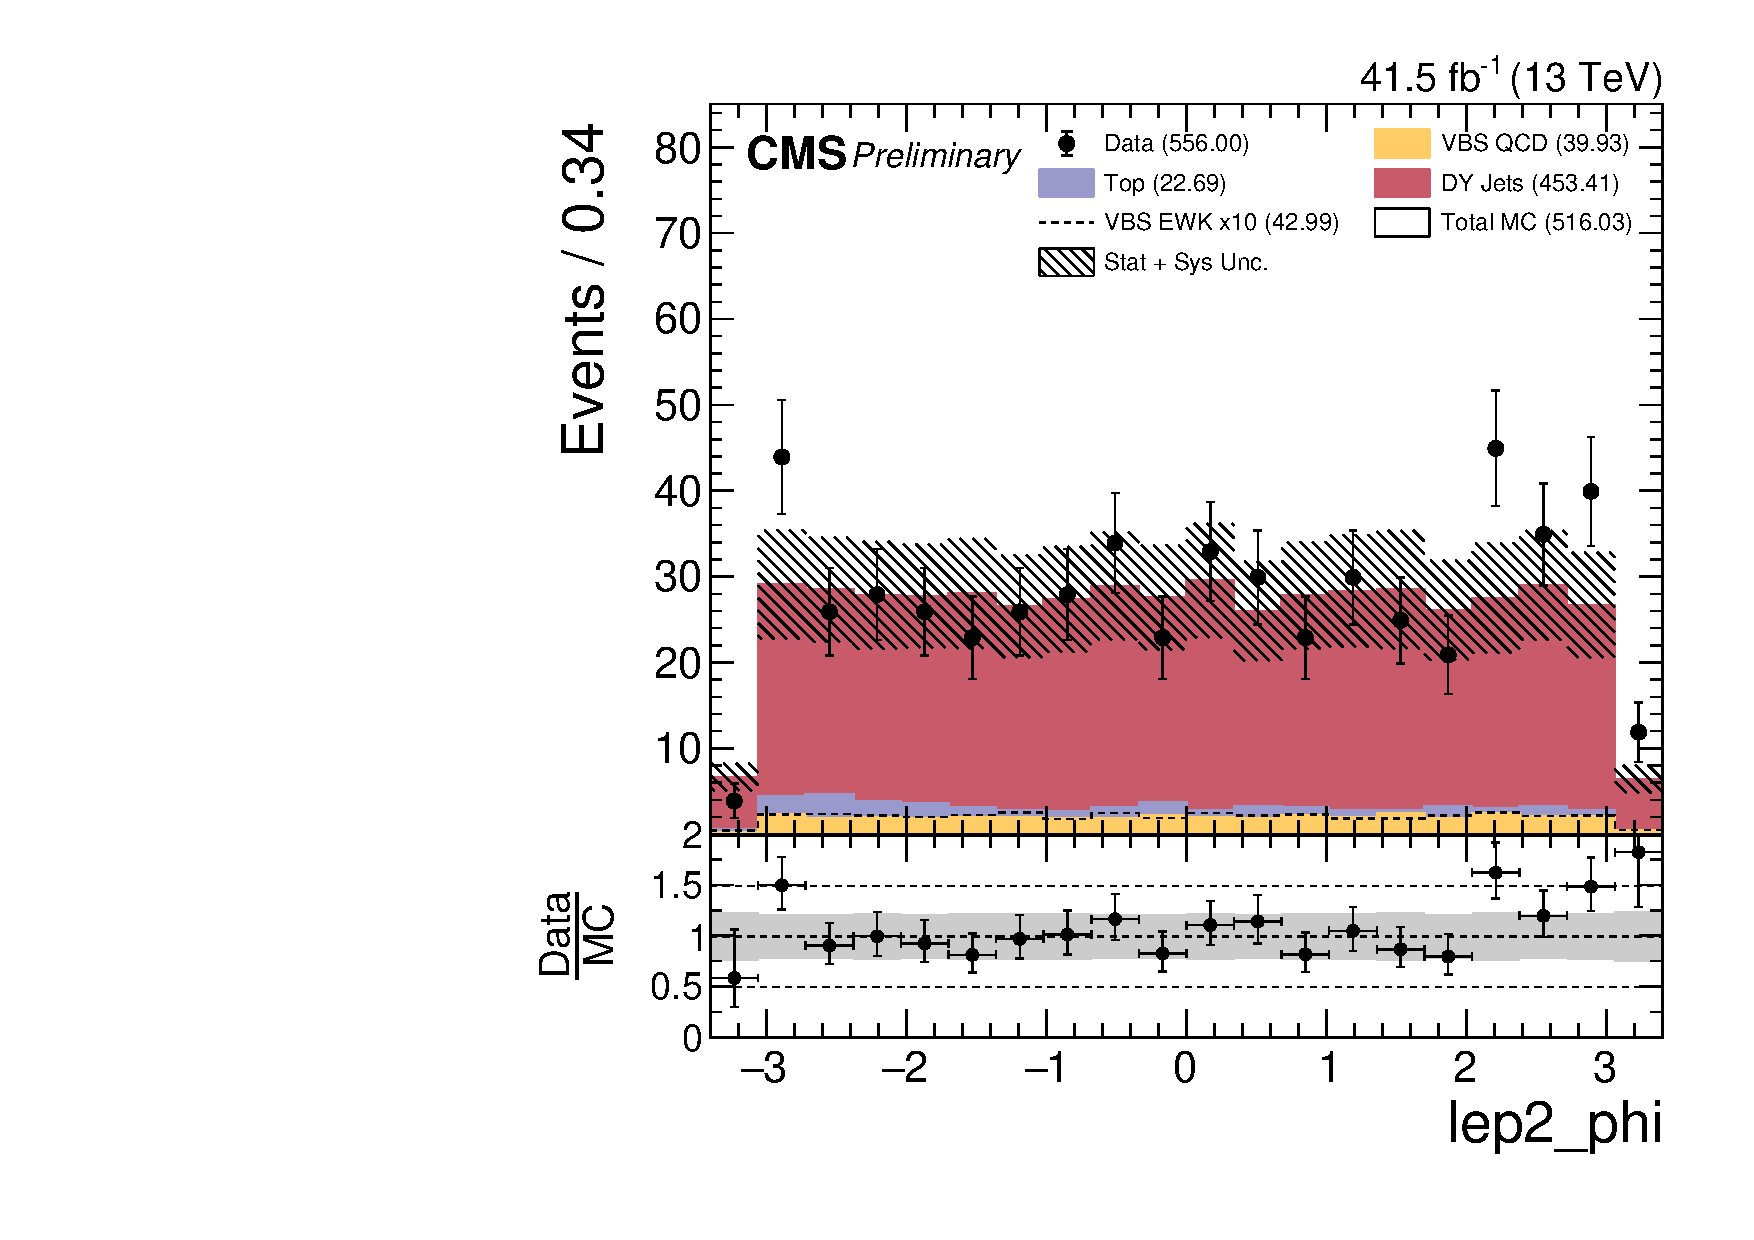
\includegraphics[width=0.335\textwidth]{analysis_plots/2017_zv/cr_vjets_m/lep2_phi.pdf} \hspace{-10pt}
  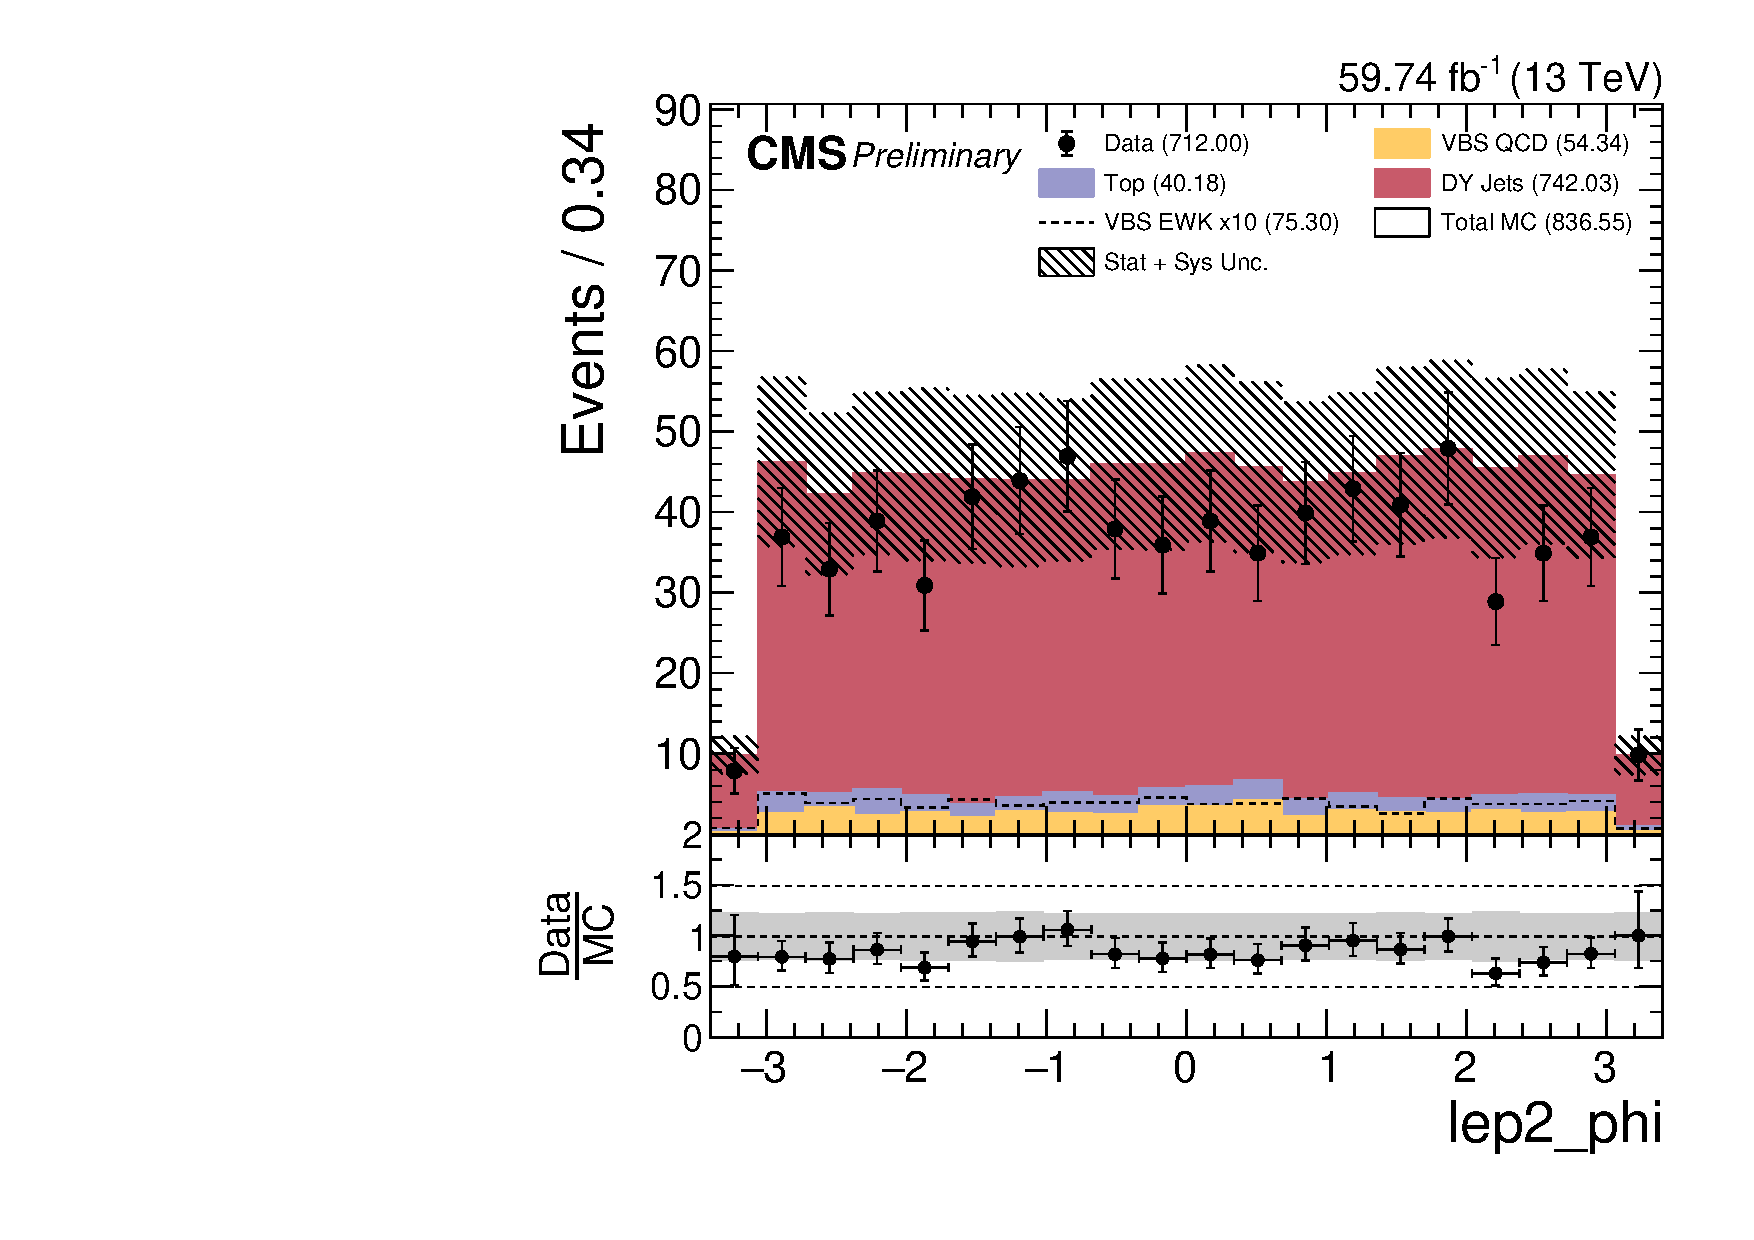
\includegraphics[width=0.335\textwidth]{analysis_plots/2018_zv/cr_vjets_m/lep2_phi.pdf} \hspace{-10pt} \\
  \caption[DY+Jets Control Region: Trailing muon kinematics in Boosted ZV Channel]%
  {DY+Jets Control Region: Trailing muon kinematics in Boosted ZV Channel.
    Error bars include statistical uncertainty on total background,
    JES and QCD scale systematic on DY+Jets and VBS\_QCD MC\@. From Left to Right: 2016,
    2017, and 2018. From Top to Bottom: \( p_T \), \( \eta \), and \( \phi \).}%
  \label{fig:zv-cr-vjets-m-lep2-pt-eta-phi}
\end{figure}

\begin{figure}[!ht]
  \centering
  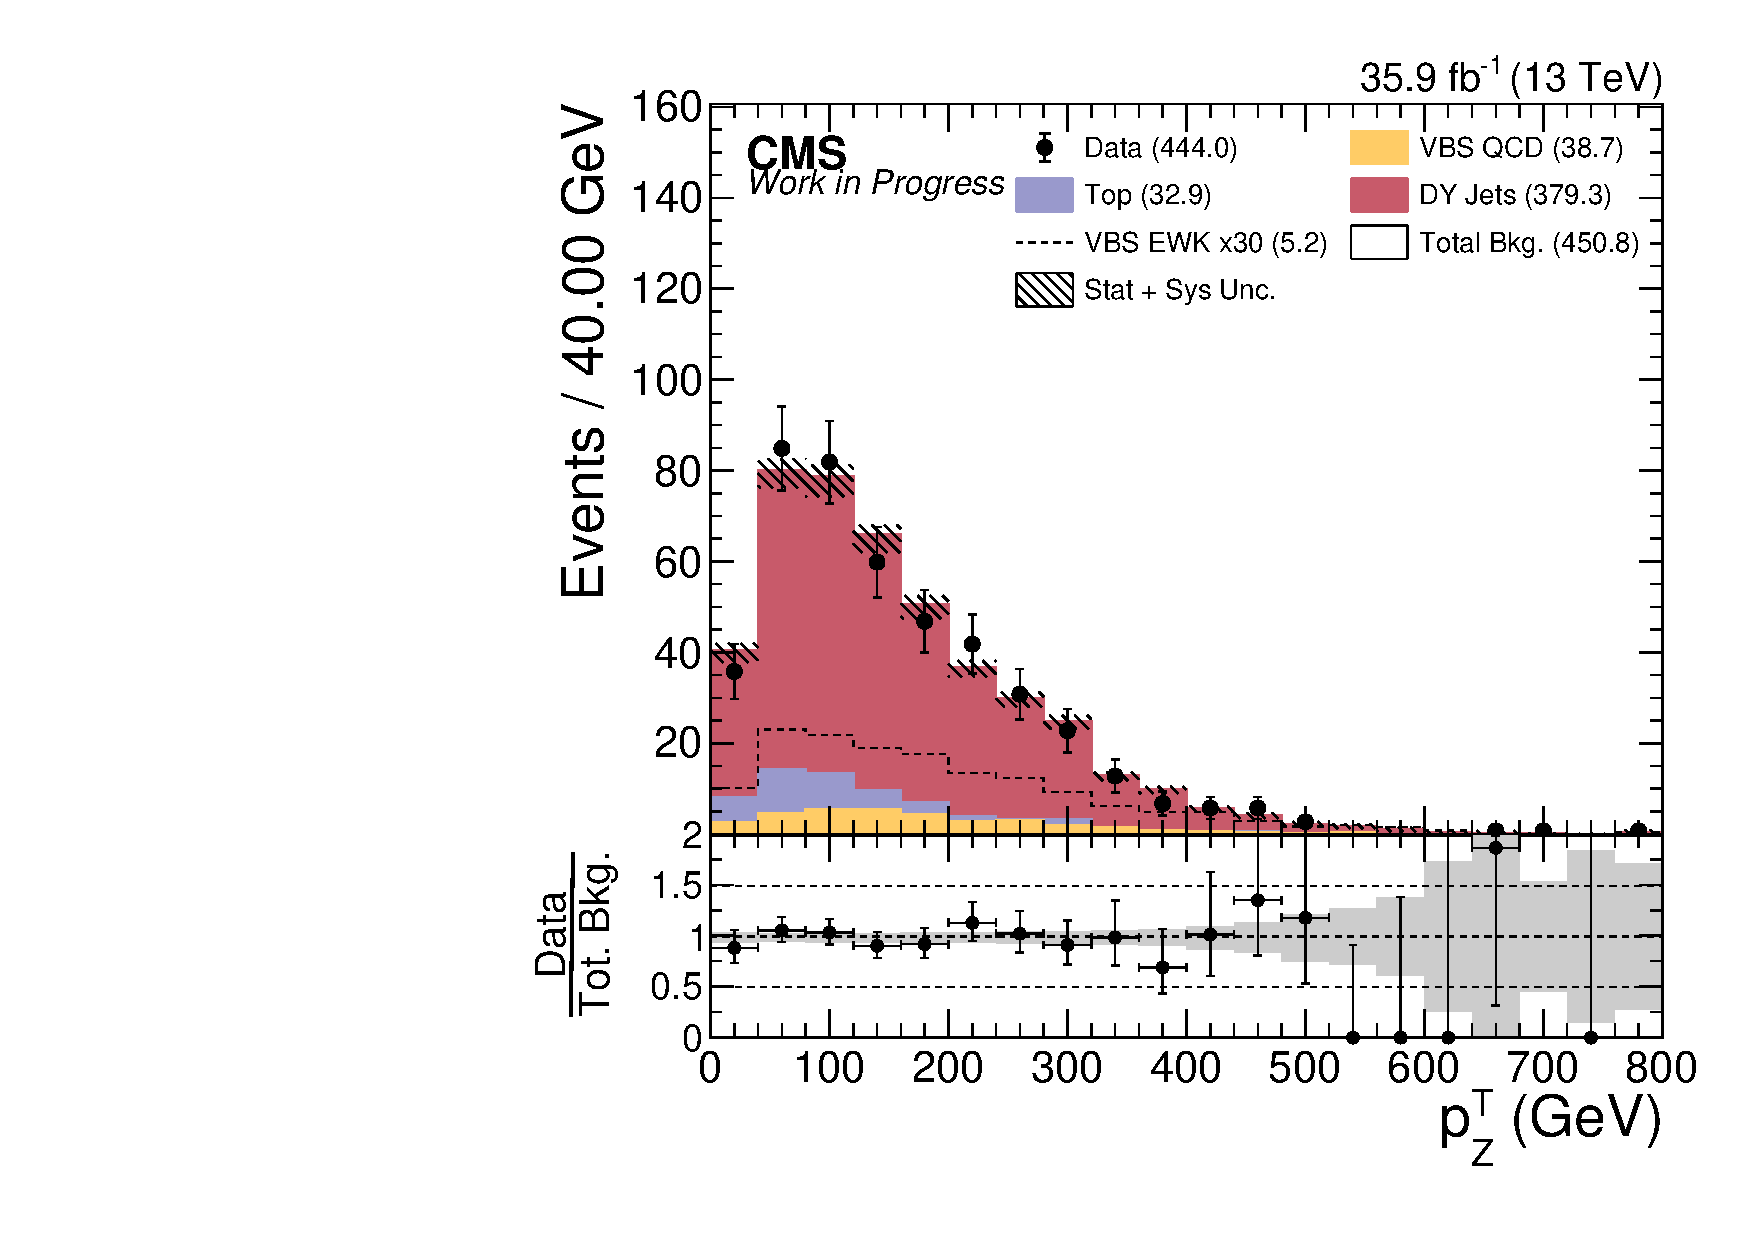
\includegraphics[width=0.335\textwidth]{analysis_plots/2016_zv/cr_vjets_l/v_lep_pt.pdf} \hspace{-10pt}
  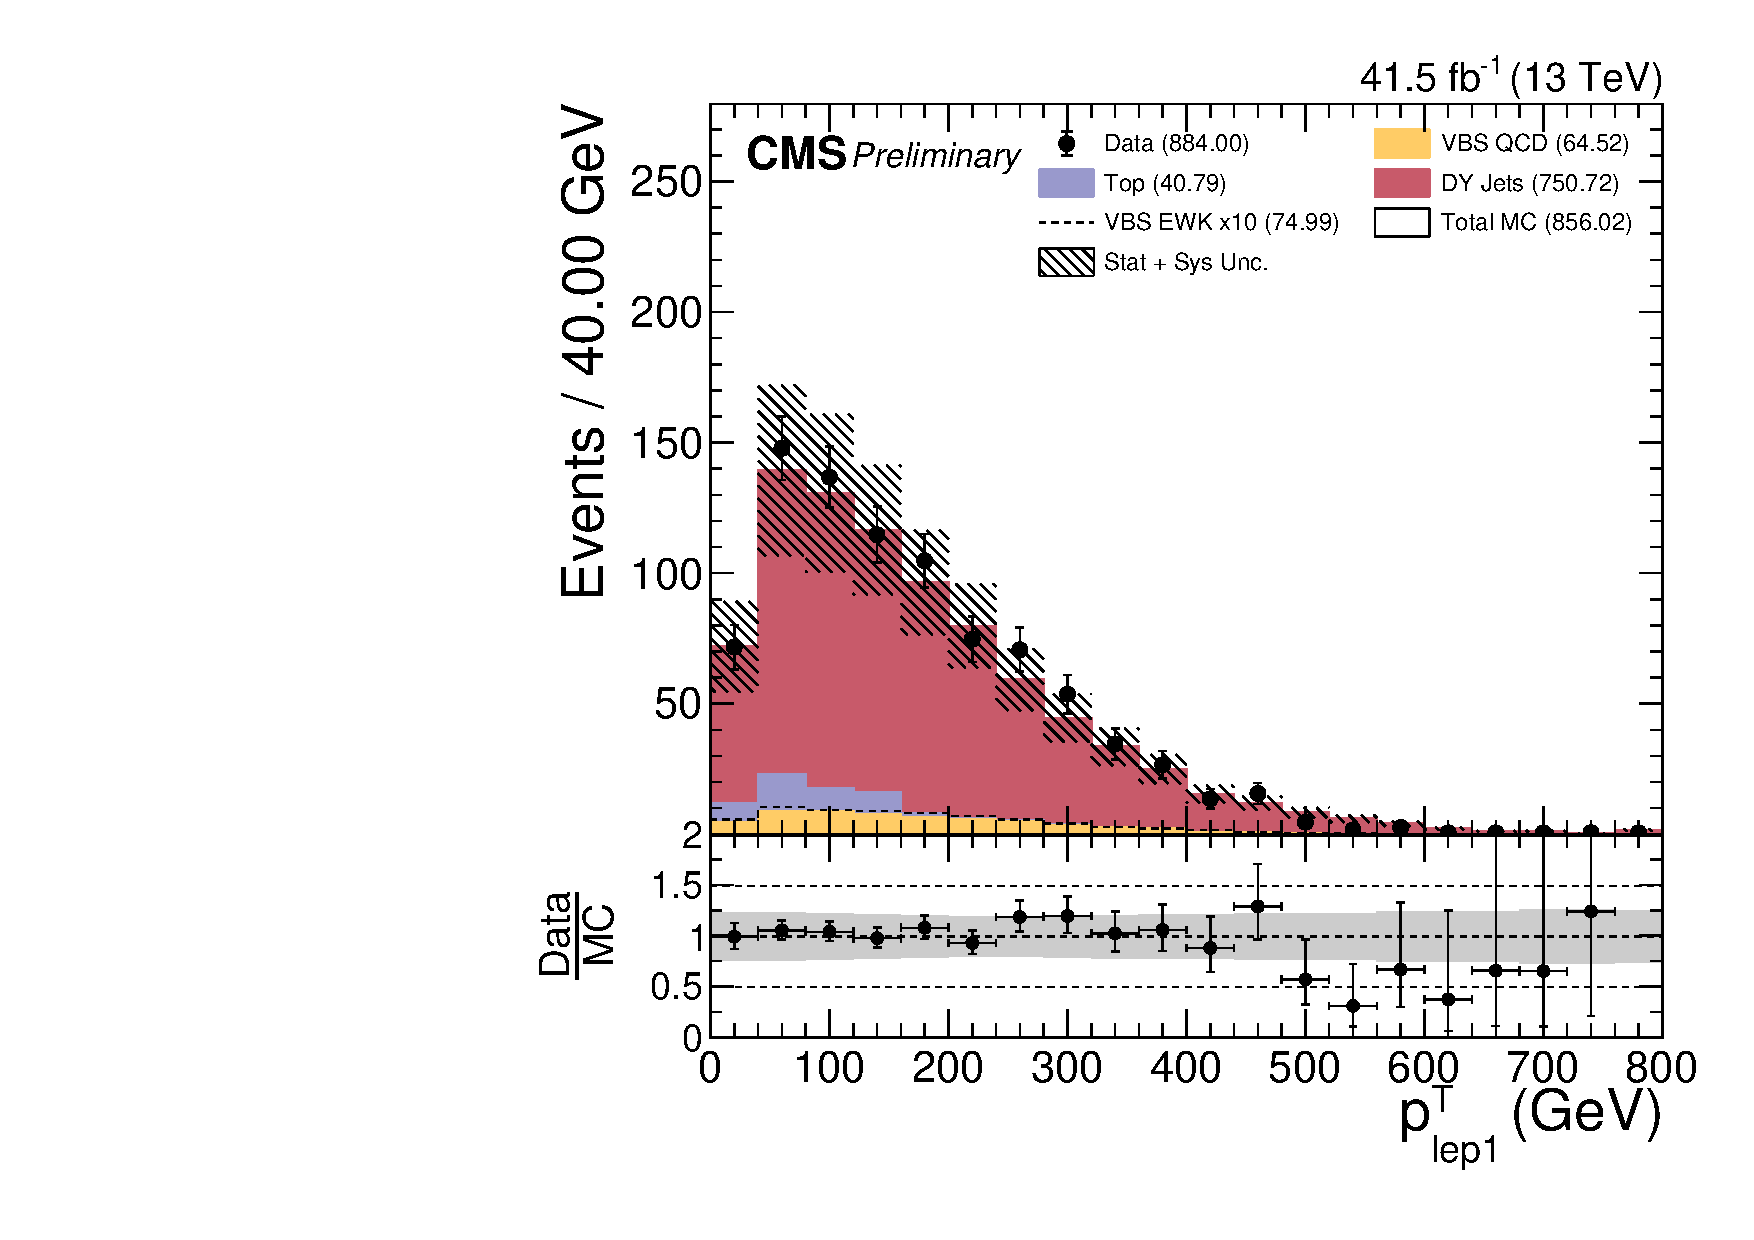
\includegraphics[width=0.335\textwidth]{analysis_plots/2017_zv/cr_vjets_l/v_lep_pt.pdf} \hspace{-10pt}
  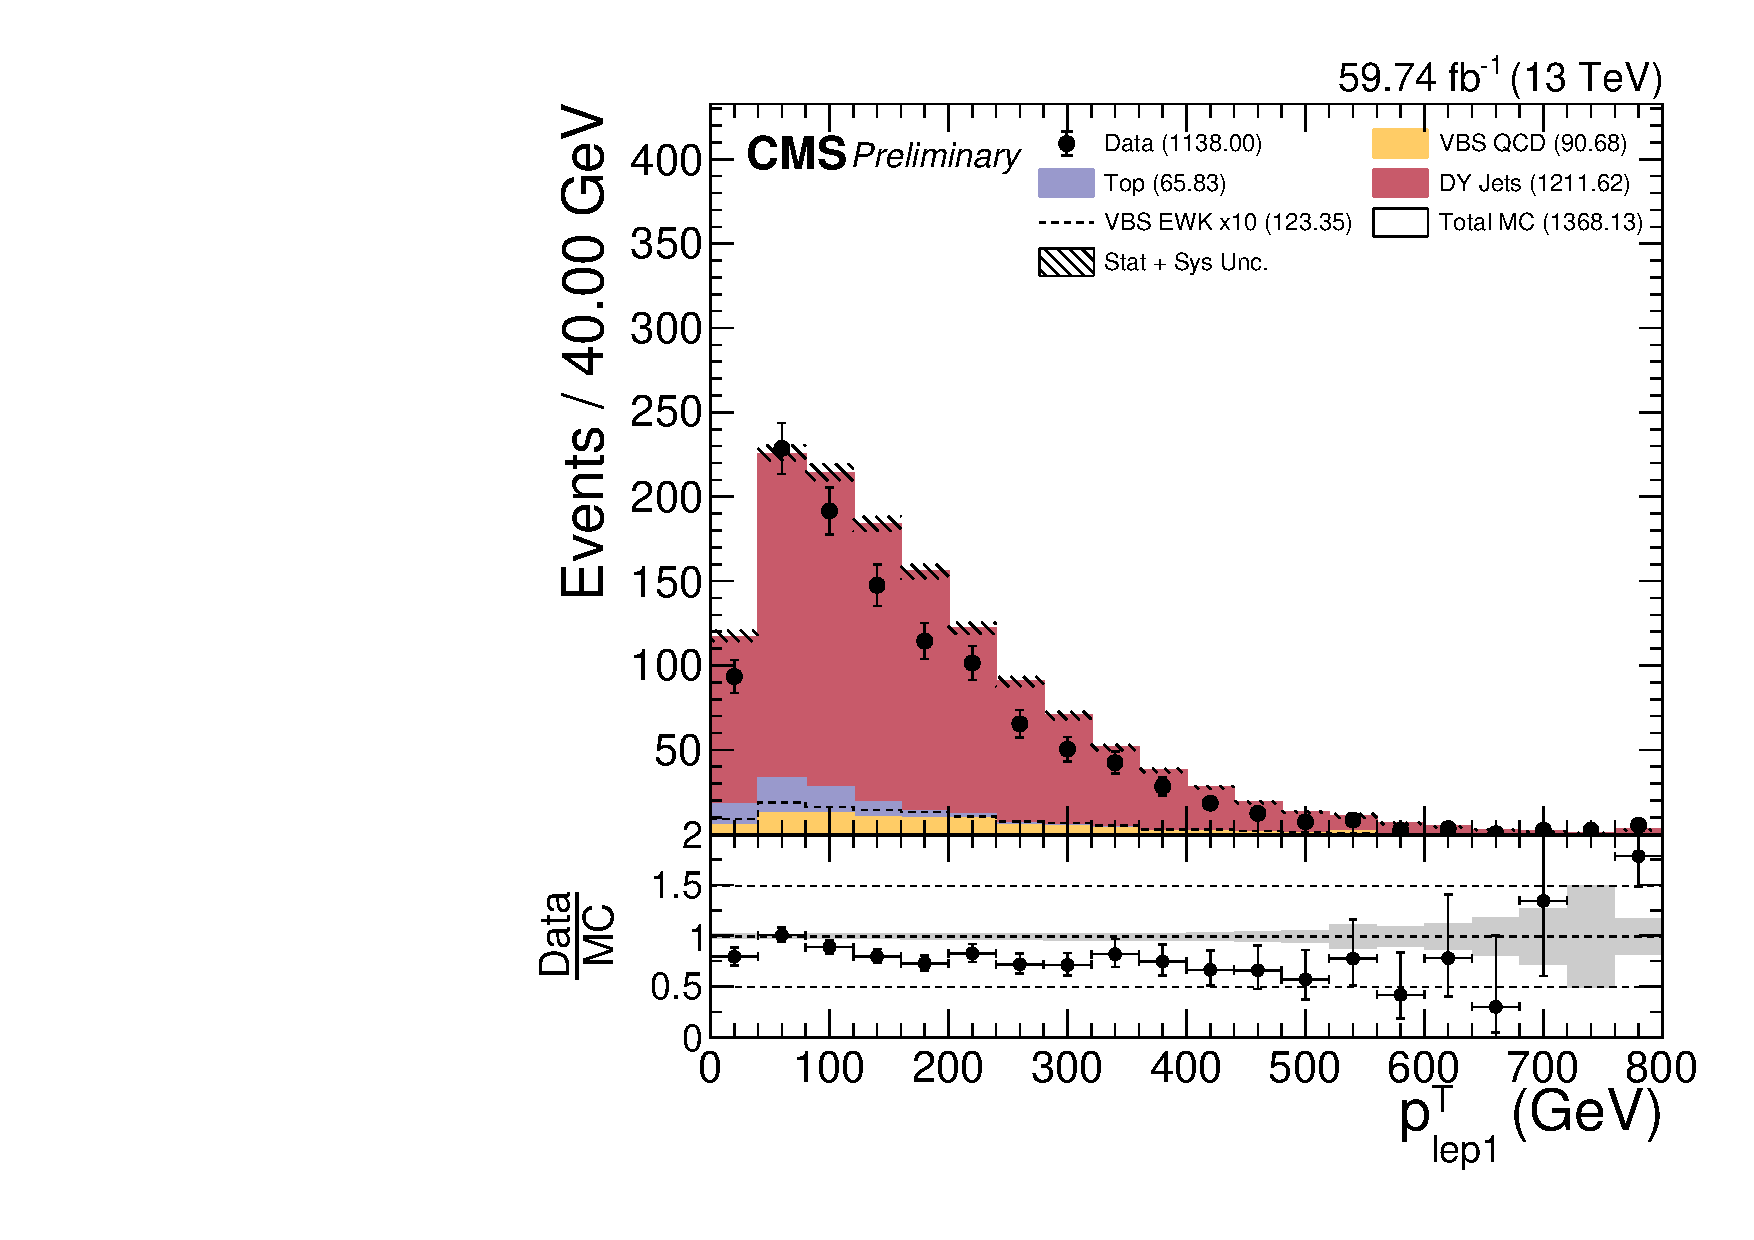
\includegraphics[width=0.335\textwidth]{analysis_plots/2018_zv/cr_vjets_l/v_lep_pt.pdf} \hspace{-10pt} \\
  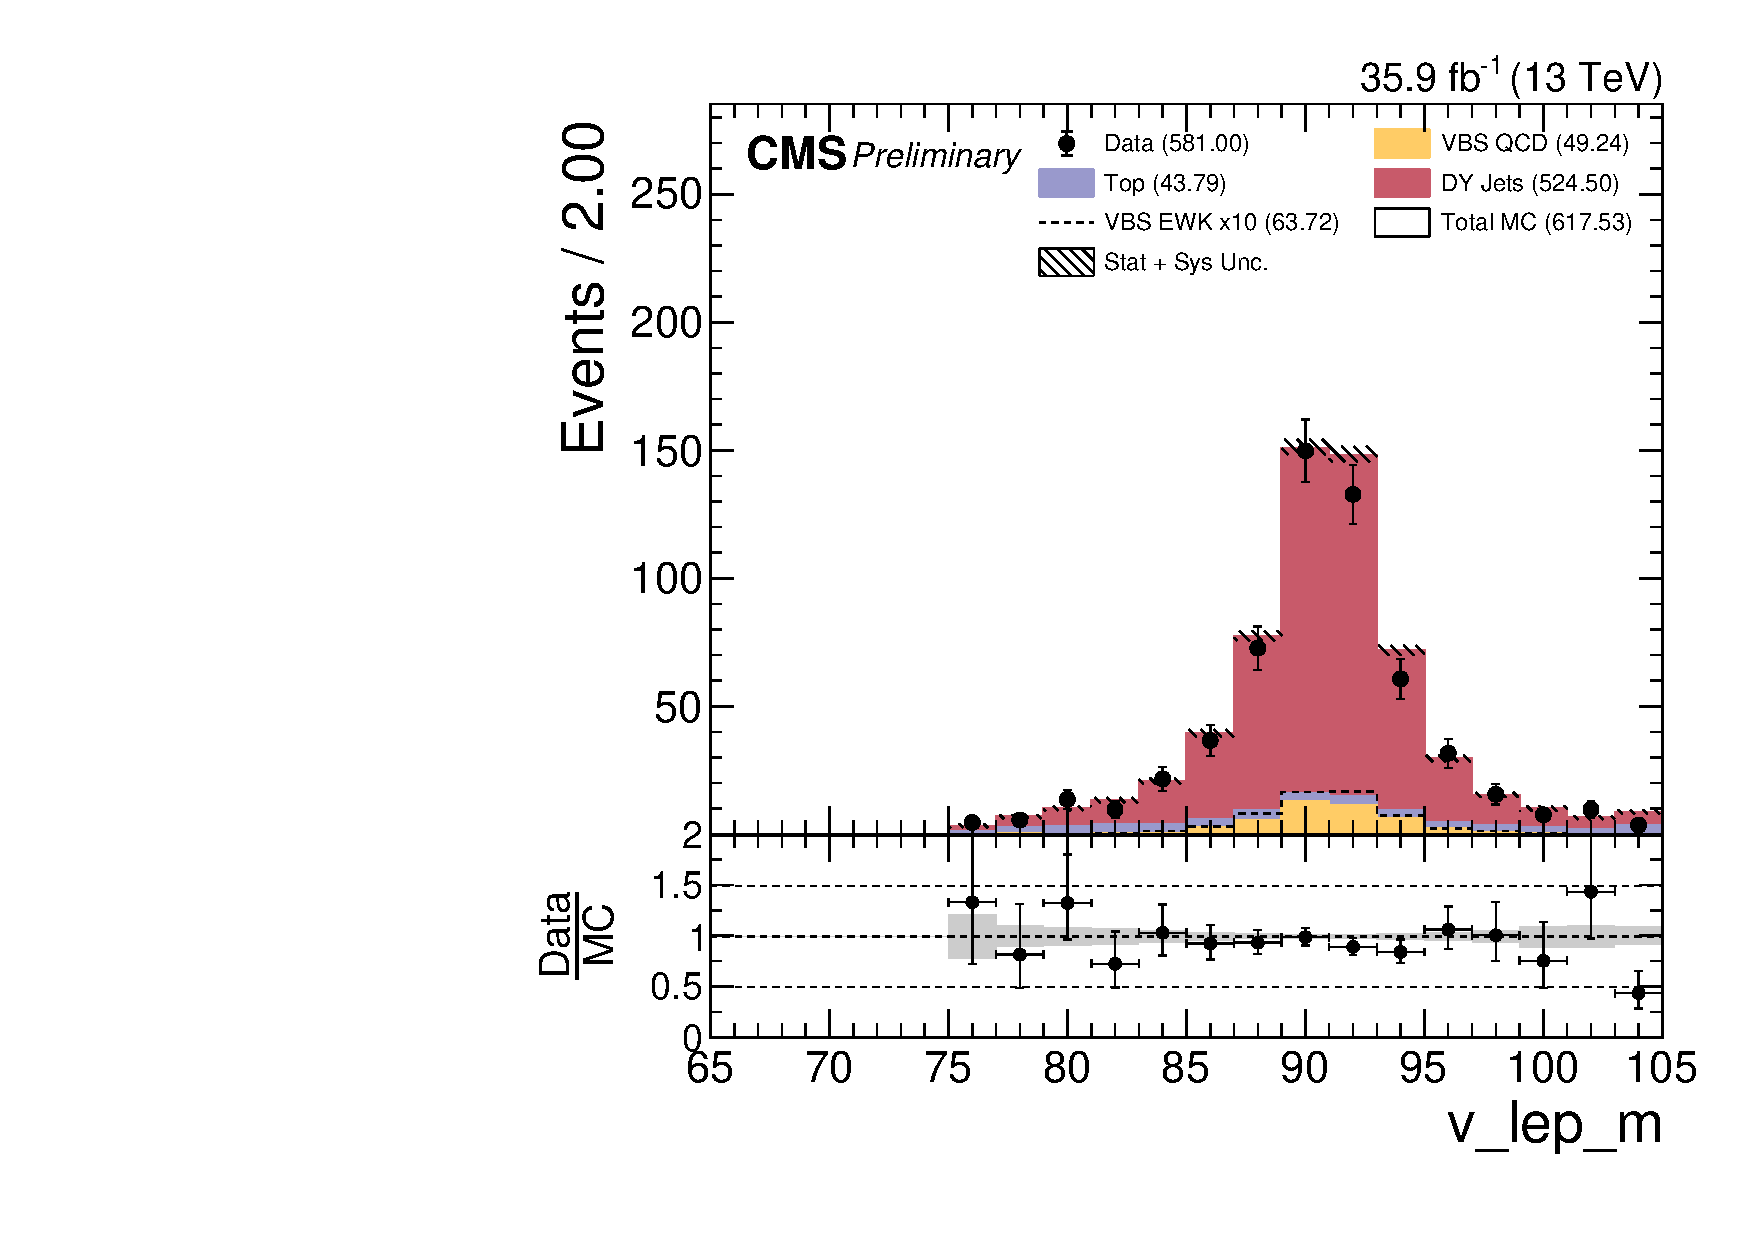
\includegraphics[width=0.335\textwidth]{analysis_plots/2016_zv/cr_vjets_l/v_lep_m.pdf} \hspace{-10pt}
  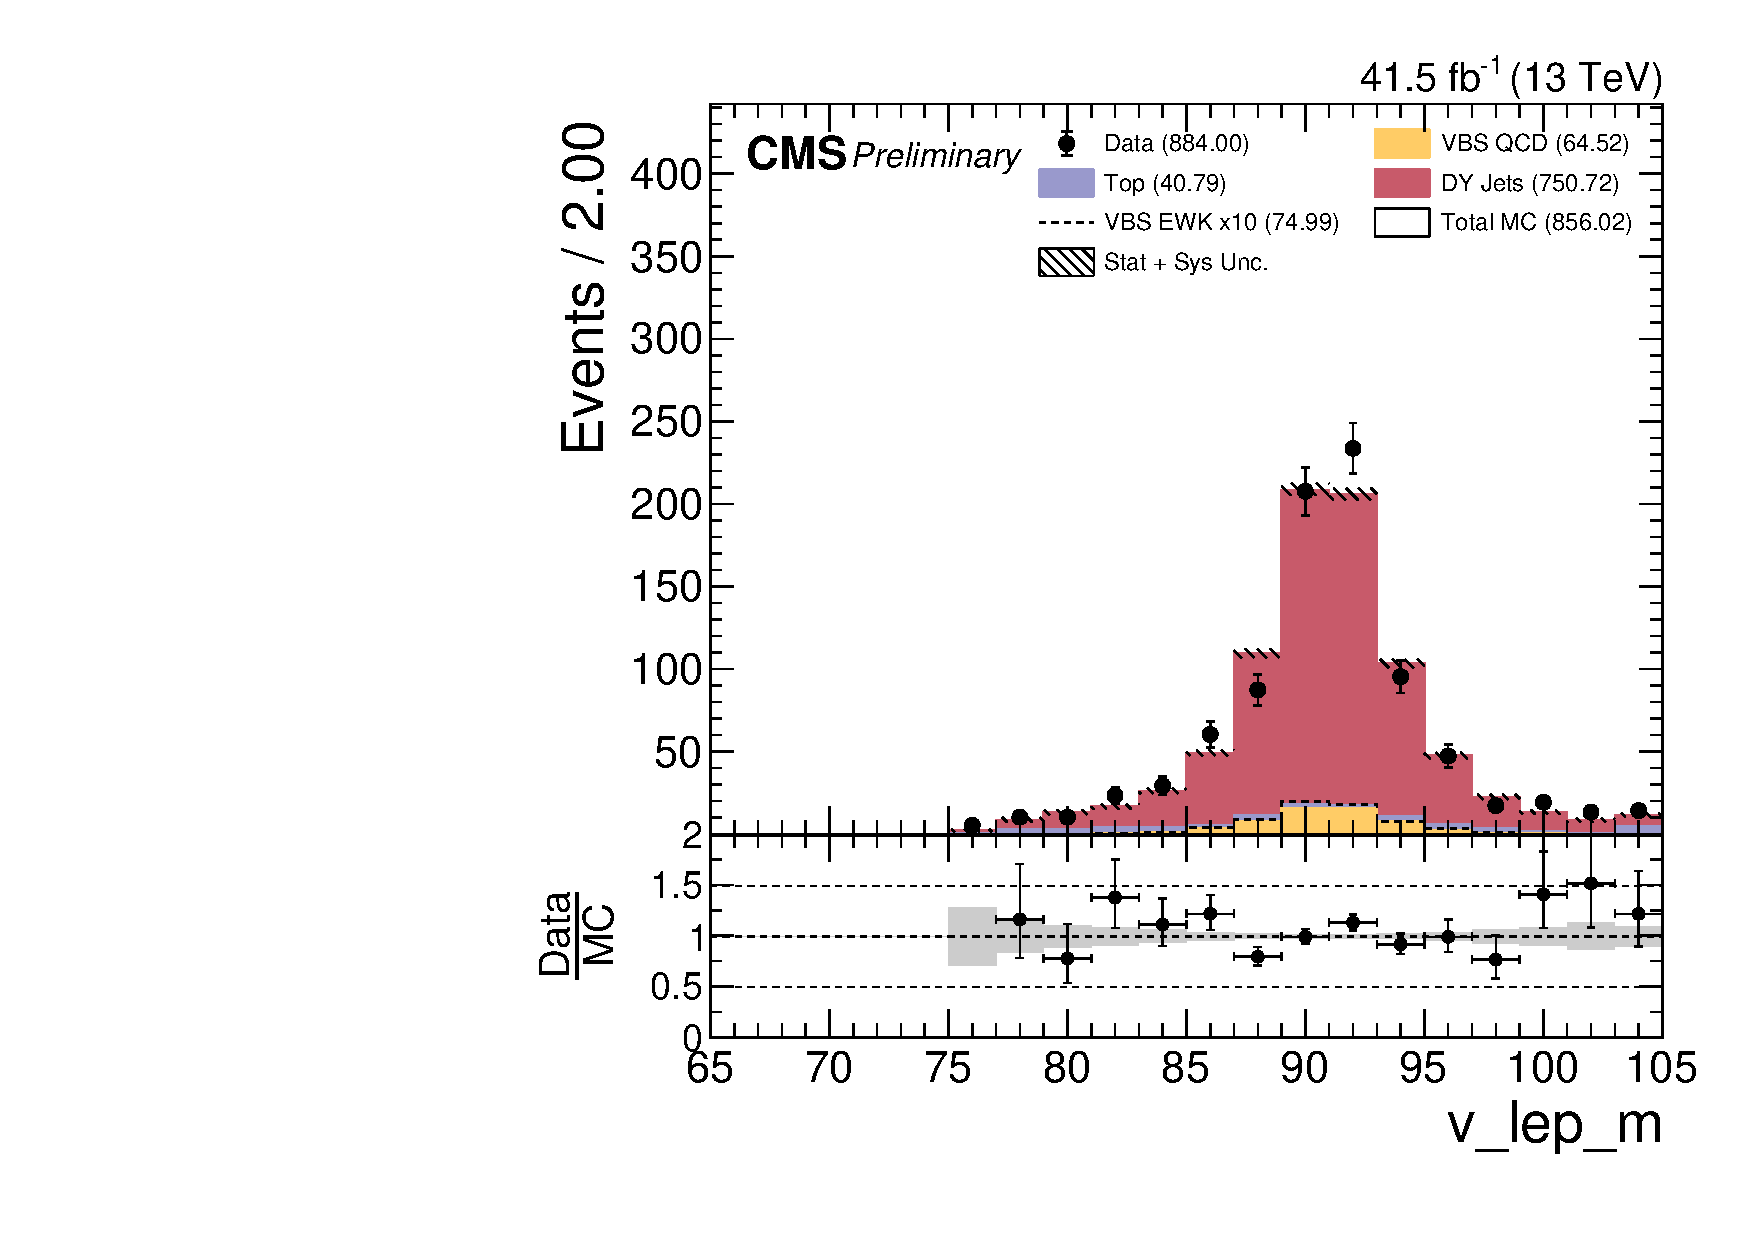
\includegraphics[width=0.335\textwidth]{analysis_plots/2017_zv/cr_vjets_l/v_lep_m.pdf} \hspace{-10pt}
  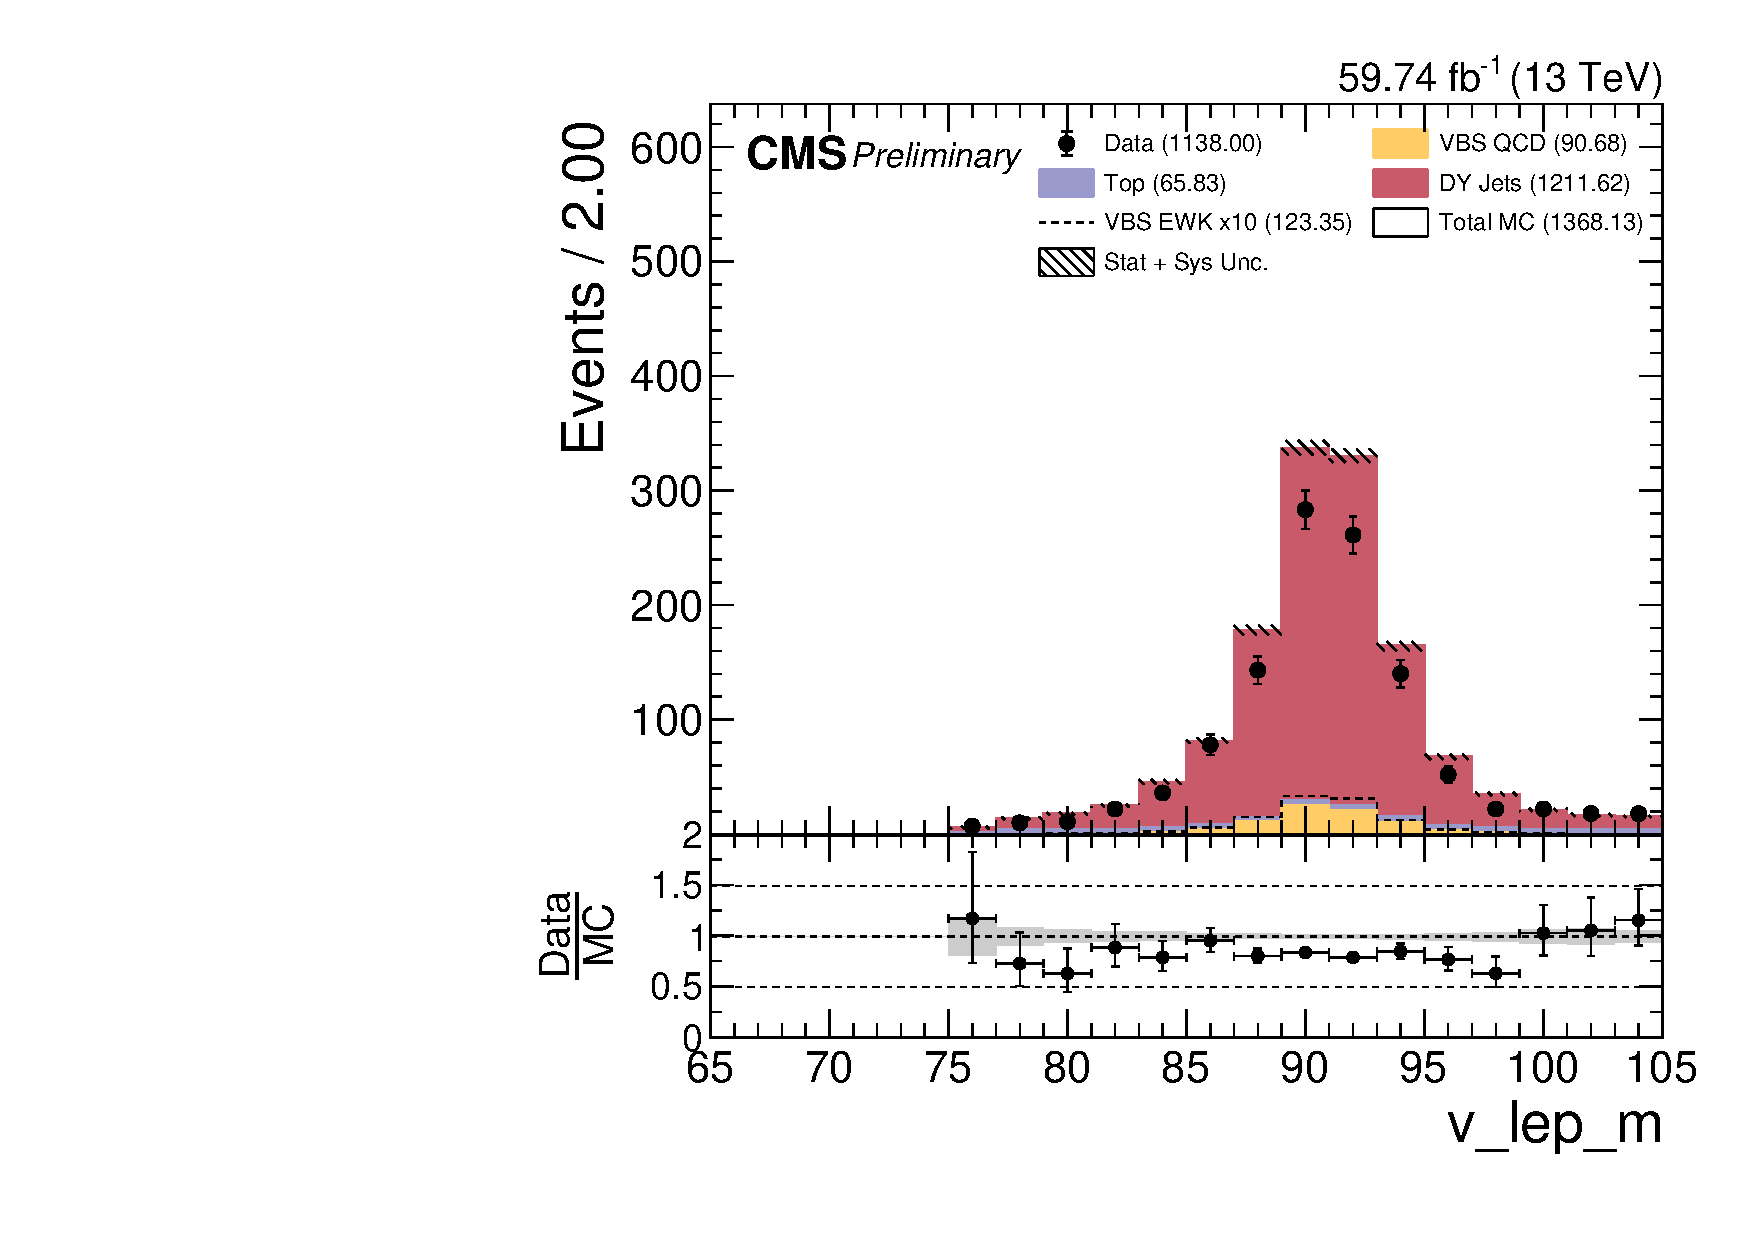
\includegraphics[width=0.335\textwidth]{analysis_plots/2018_zv/cr_vjets_l/v_lep_m.pdf} \hspace{-10pt} \\
  \caption[DY+Jets Control Region: \textit{Z} boson kinematics in Boosted ZV Channel]%
  {DY+Jets Control Region: \textit{Z} boson kinematics in Boosted ZV Channel.
    Error bars include statistical uncertainty on total background,
    JES and QCD scale systematic on DY+Jets and VBS\_QCD MC\@. From Left to Right: 2016,
    2017, and 2018. From Top to Bottom: \( p_T \), and mass.}%
  \label{fig:zv-cr-vjets-l-v-lep-pt-m}
\end{figure}

\clearpage
\section{
  Control Region DY+Jets Resolved ZV Channel
 }

\begin{figure}[!ht]
  \centering
  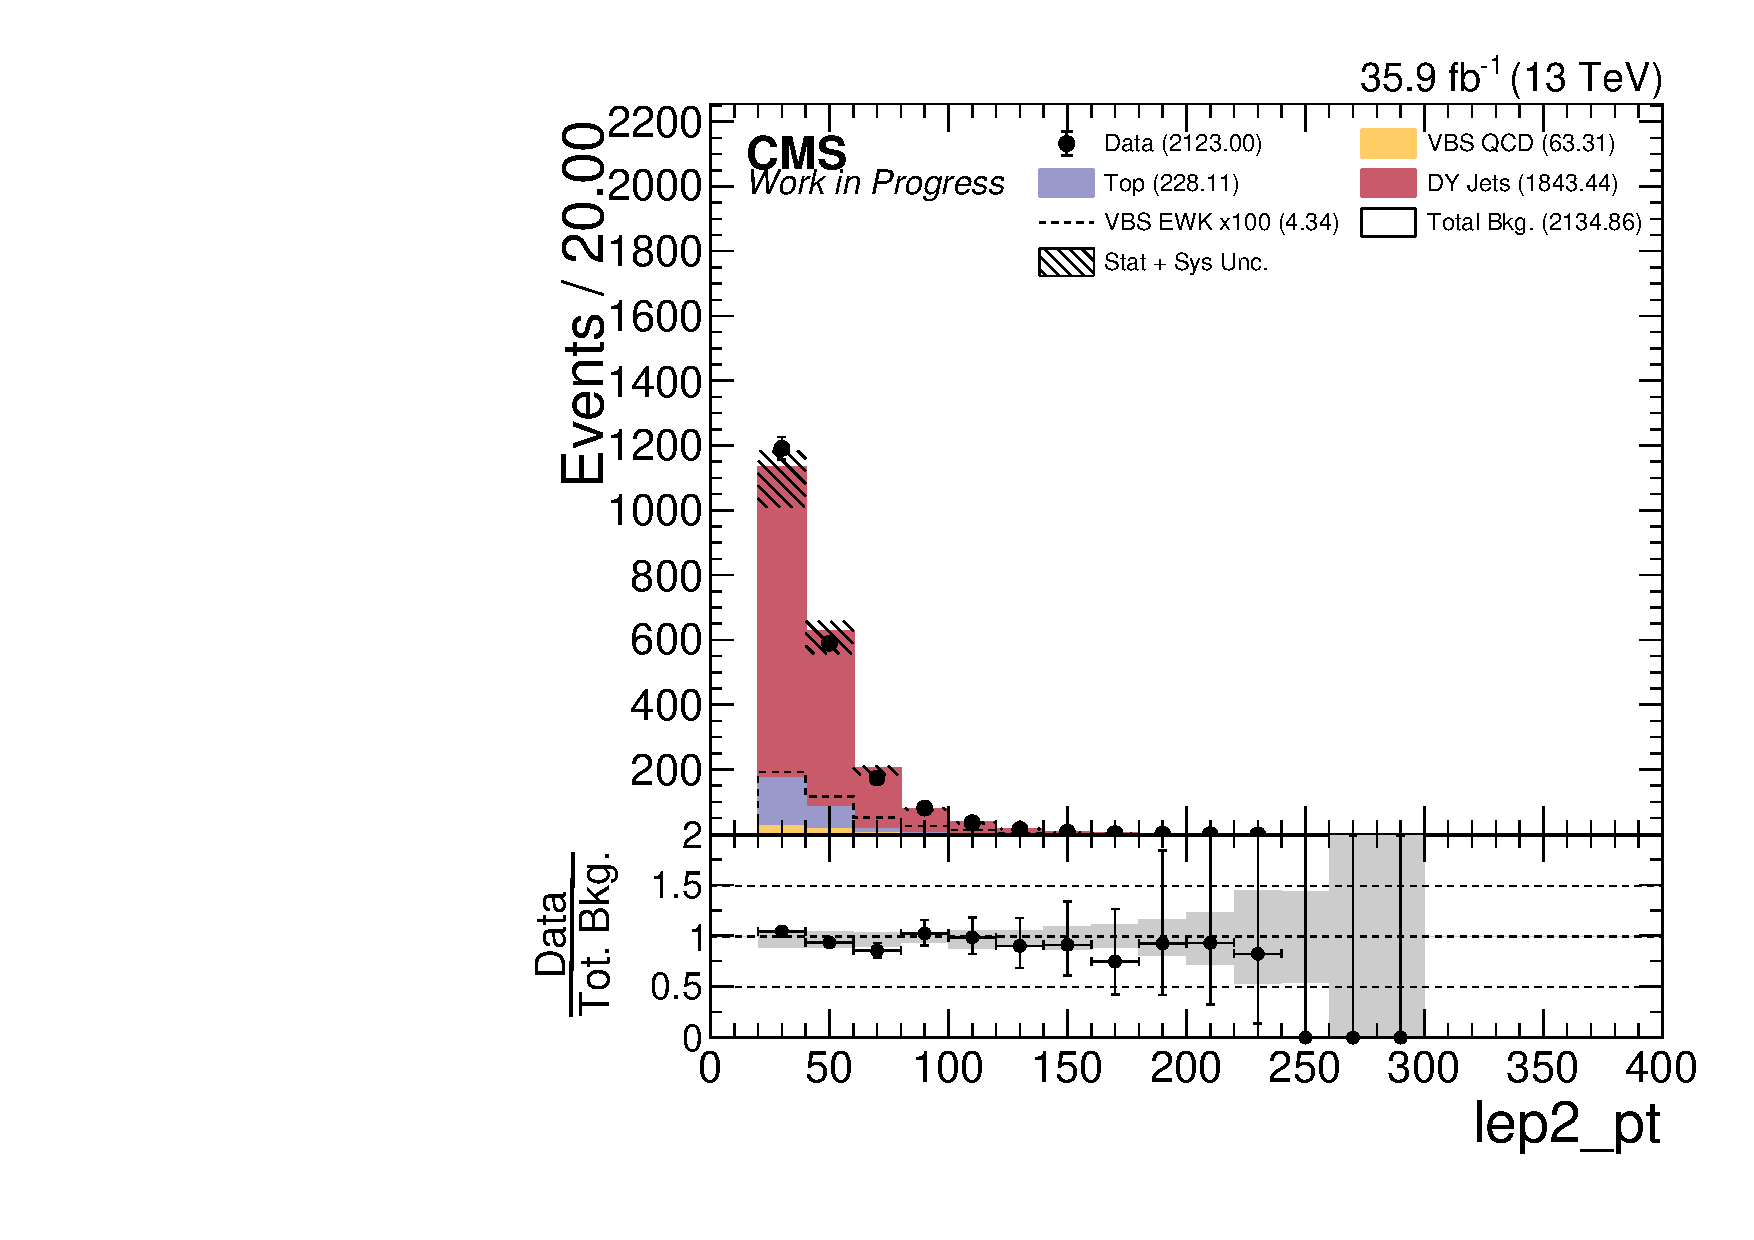
\includegraphics[width=0.335\textwidth]{analysis_plots/2016_zjj/cr_vjets_e/lep2_pt.pdf} \hspace{-10pt}
  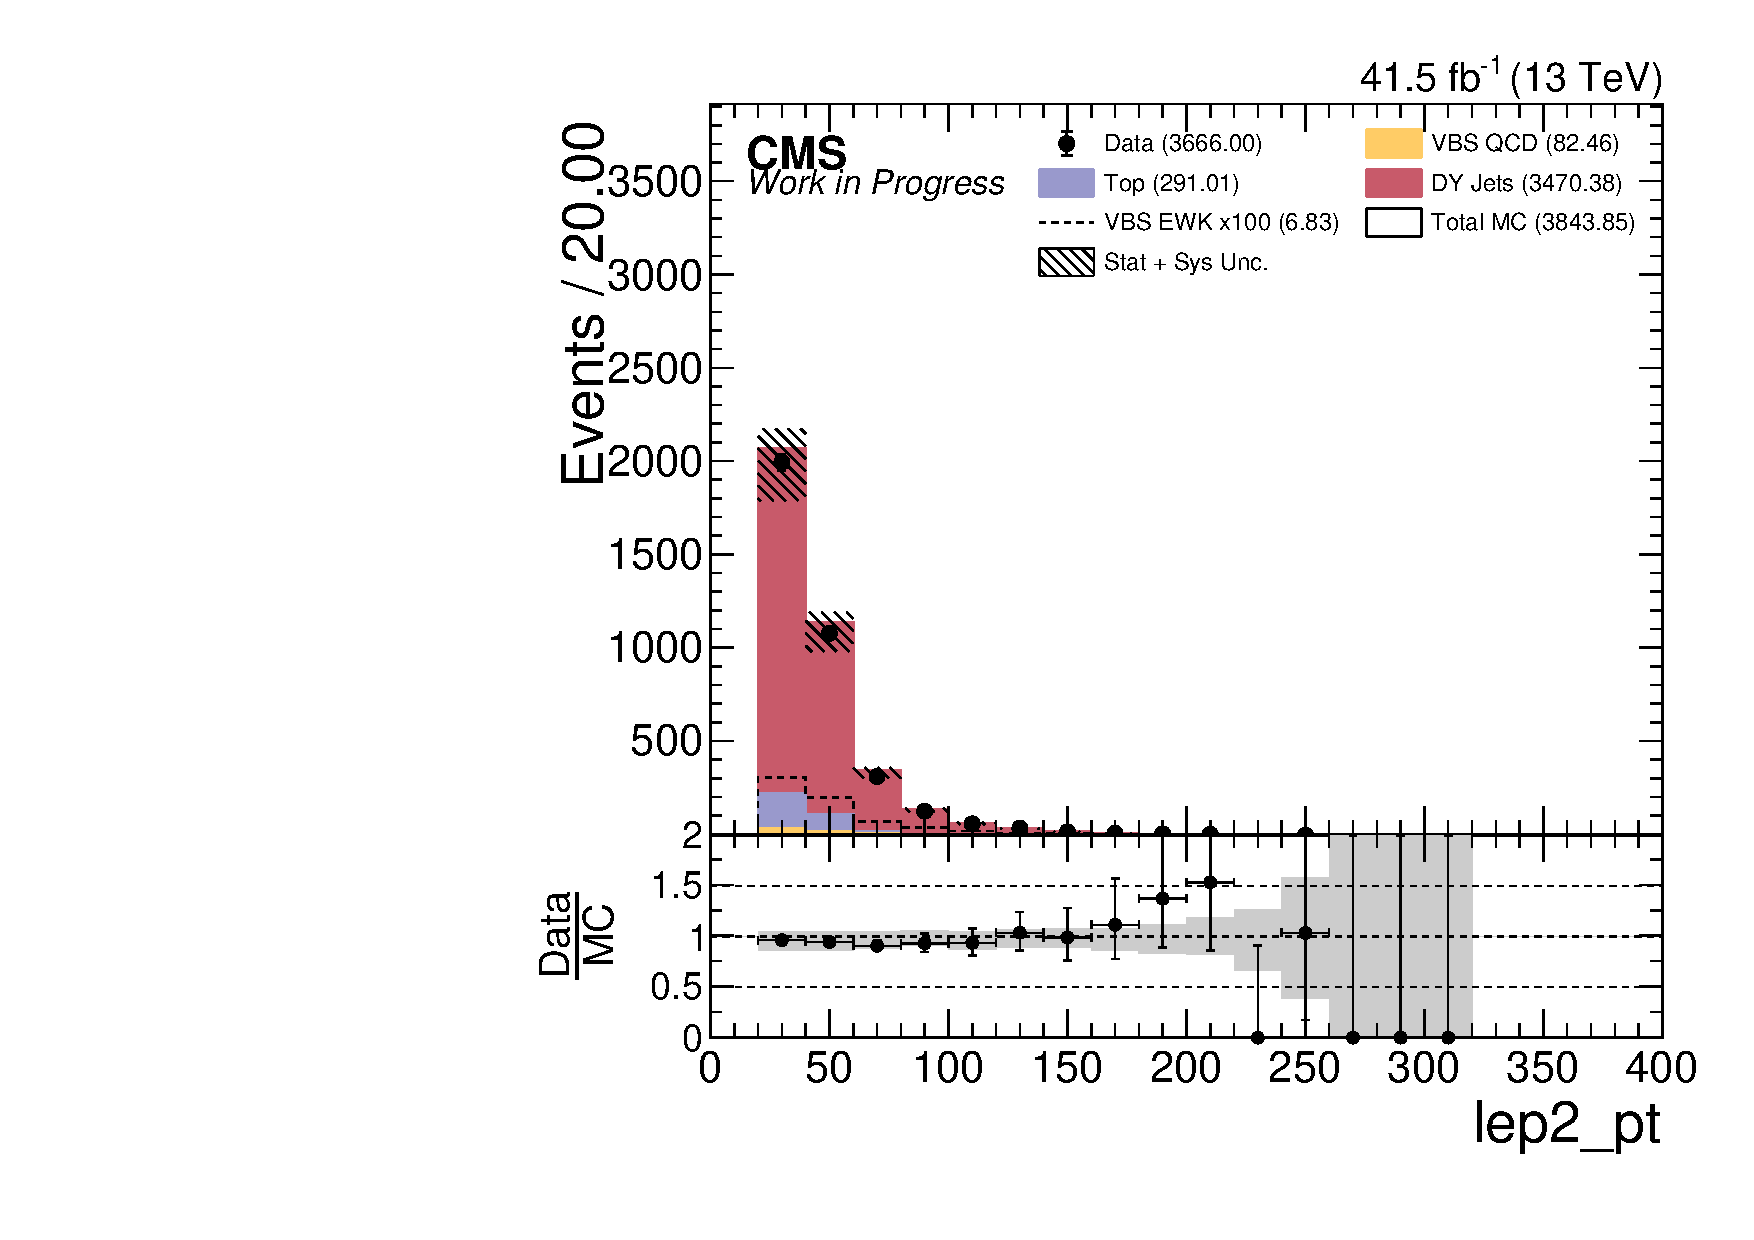
\includegraphics[width=0.335\textwidth]{analysis_plots/2017_zjj/cr_vjets_e/lep2_pt.pdf} \hspace{-10pt}
  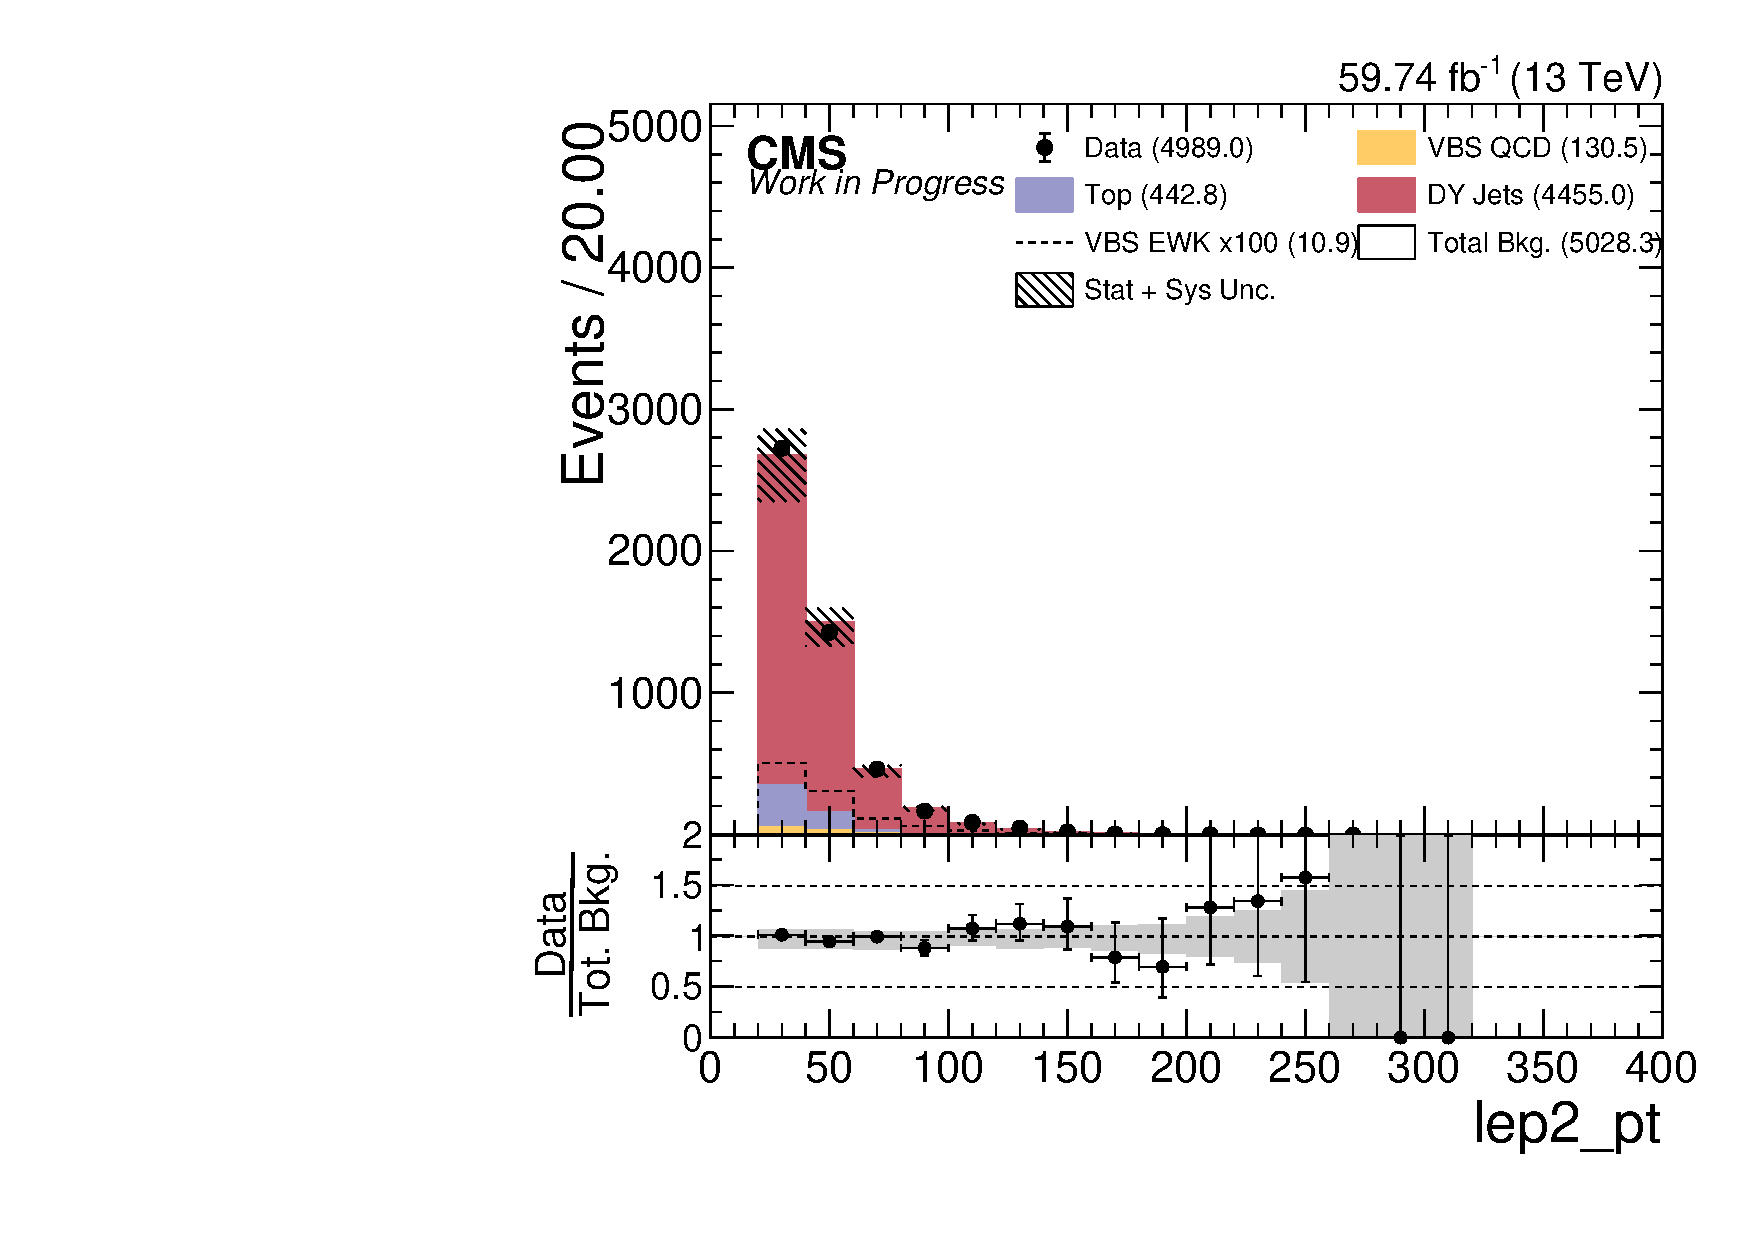
\includegraphics[width=0.335\textwidth]{analysis_plots/2018_zjj/cr_vjets_e/lep2_pt.pdf} \hspace{-10pt} \\
  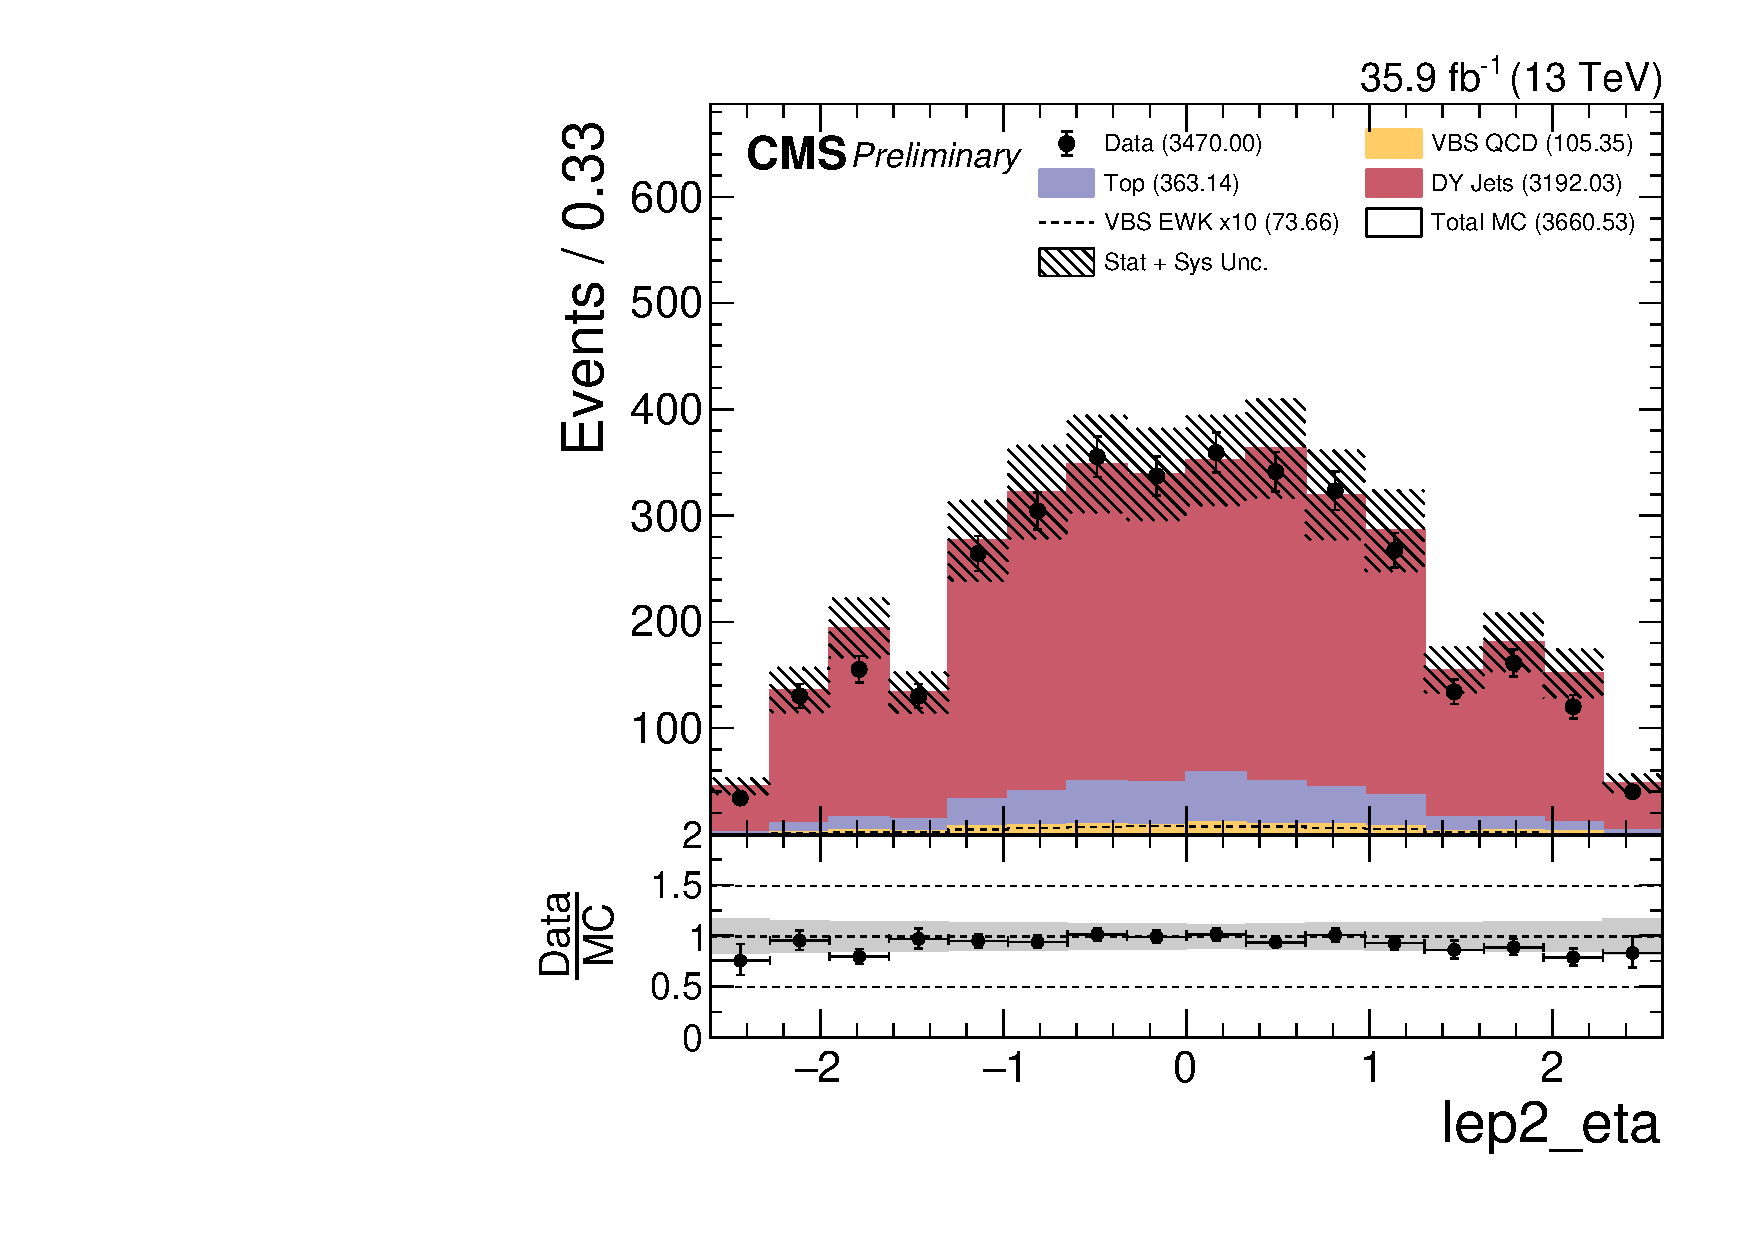
\includegraphics[width=0.335\textwidth]{analysis_plots/2016_zjj/cr_vjets_e/lep2_eta.pdf} \hspace{-10pt}
  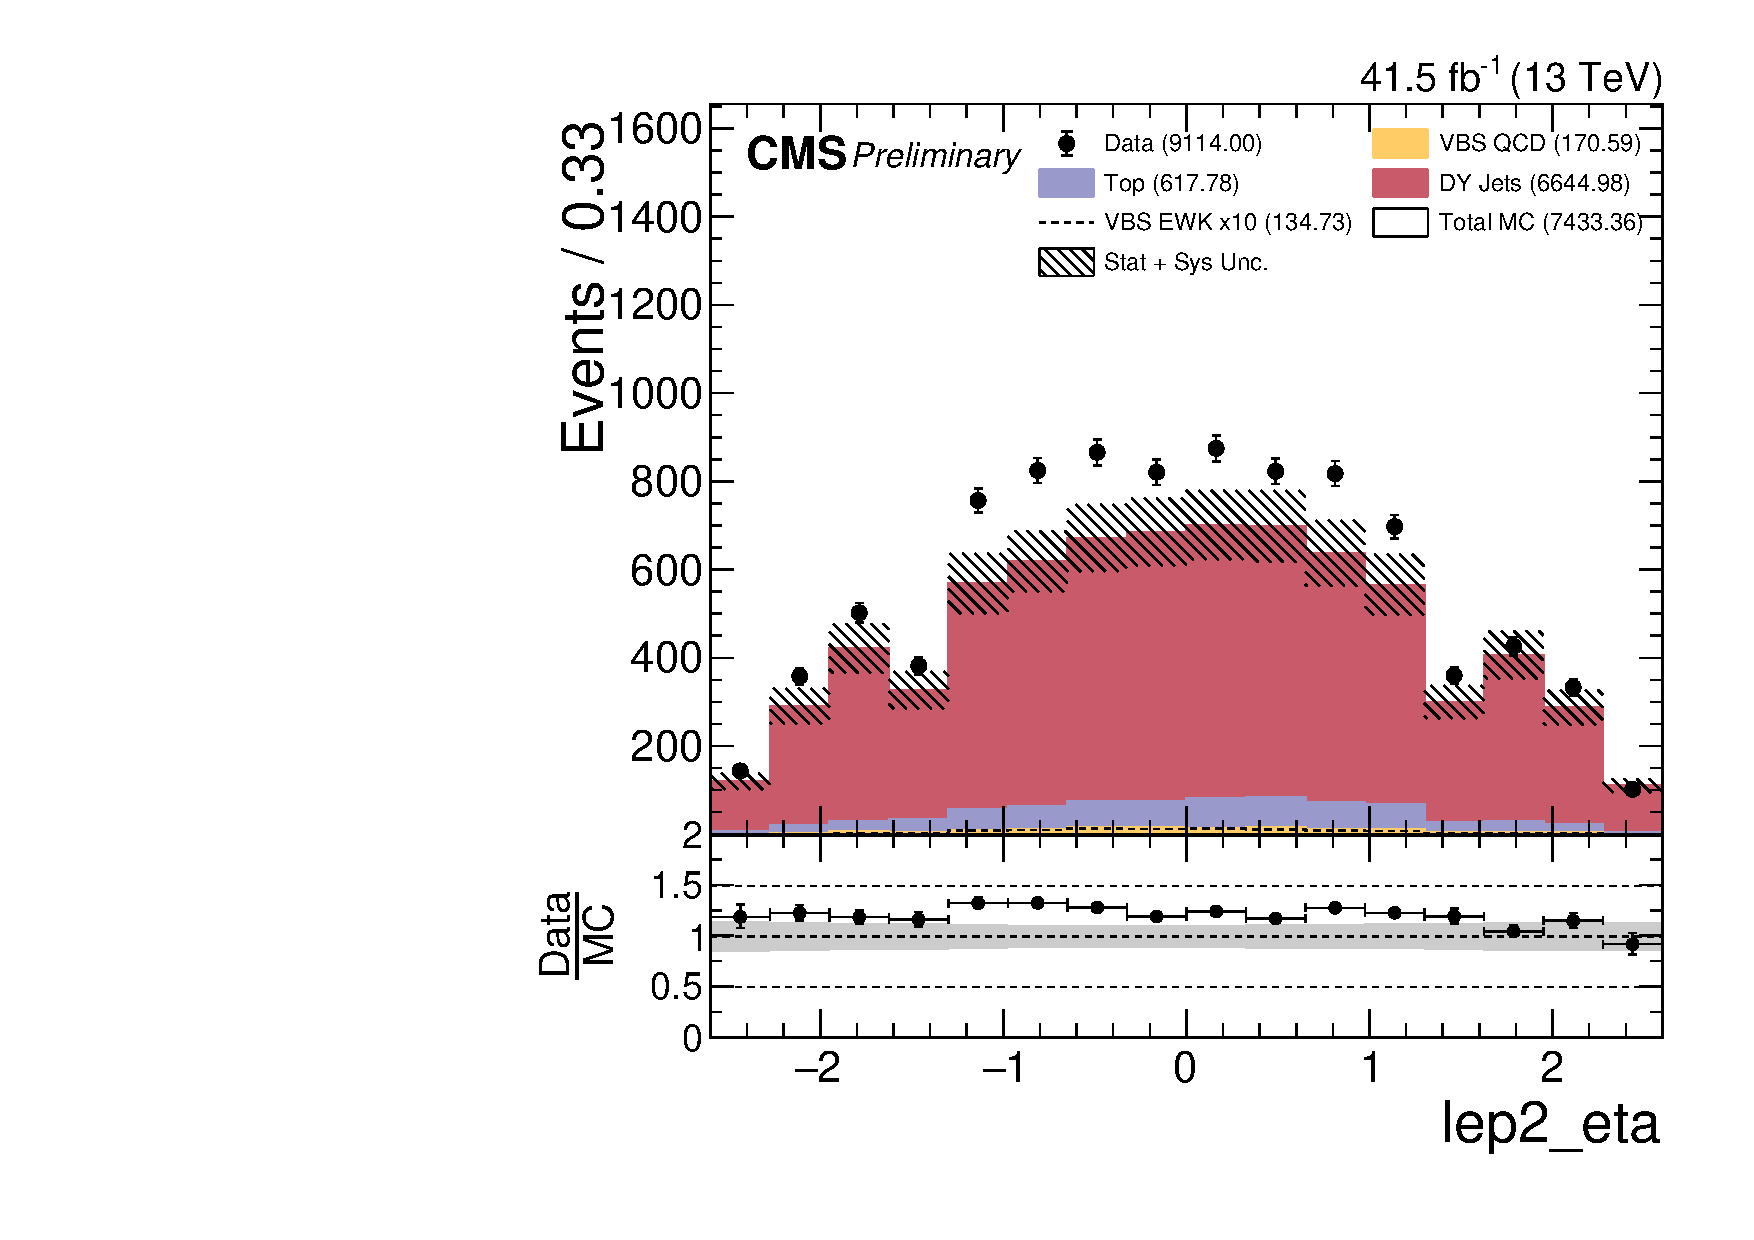
\includegraphics[width=0.335\textwidth]{analysis_plots/2017_zjj/cr_vjets_e/lep2_eta.pdf} \hspace{-10pt}
  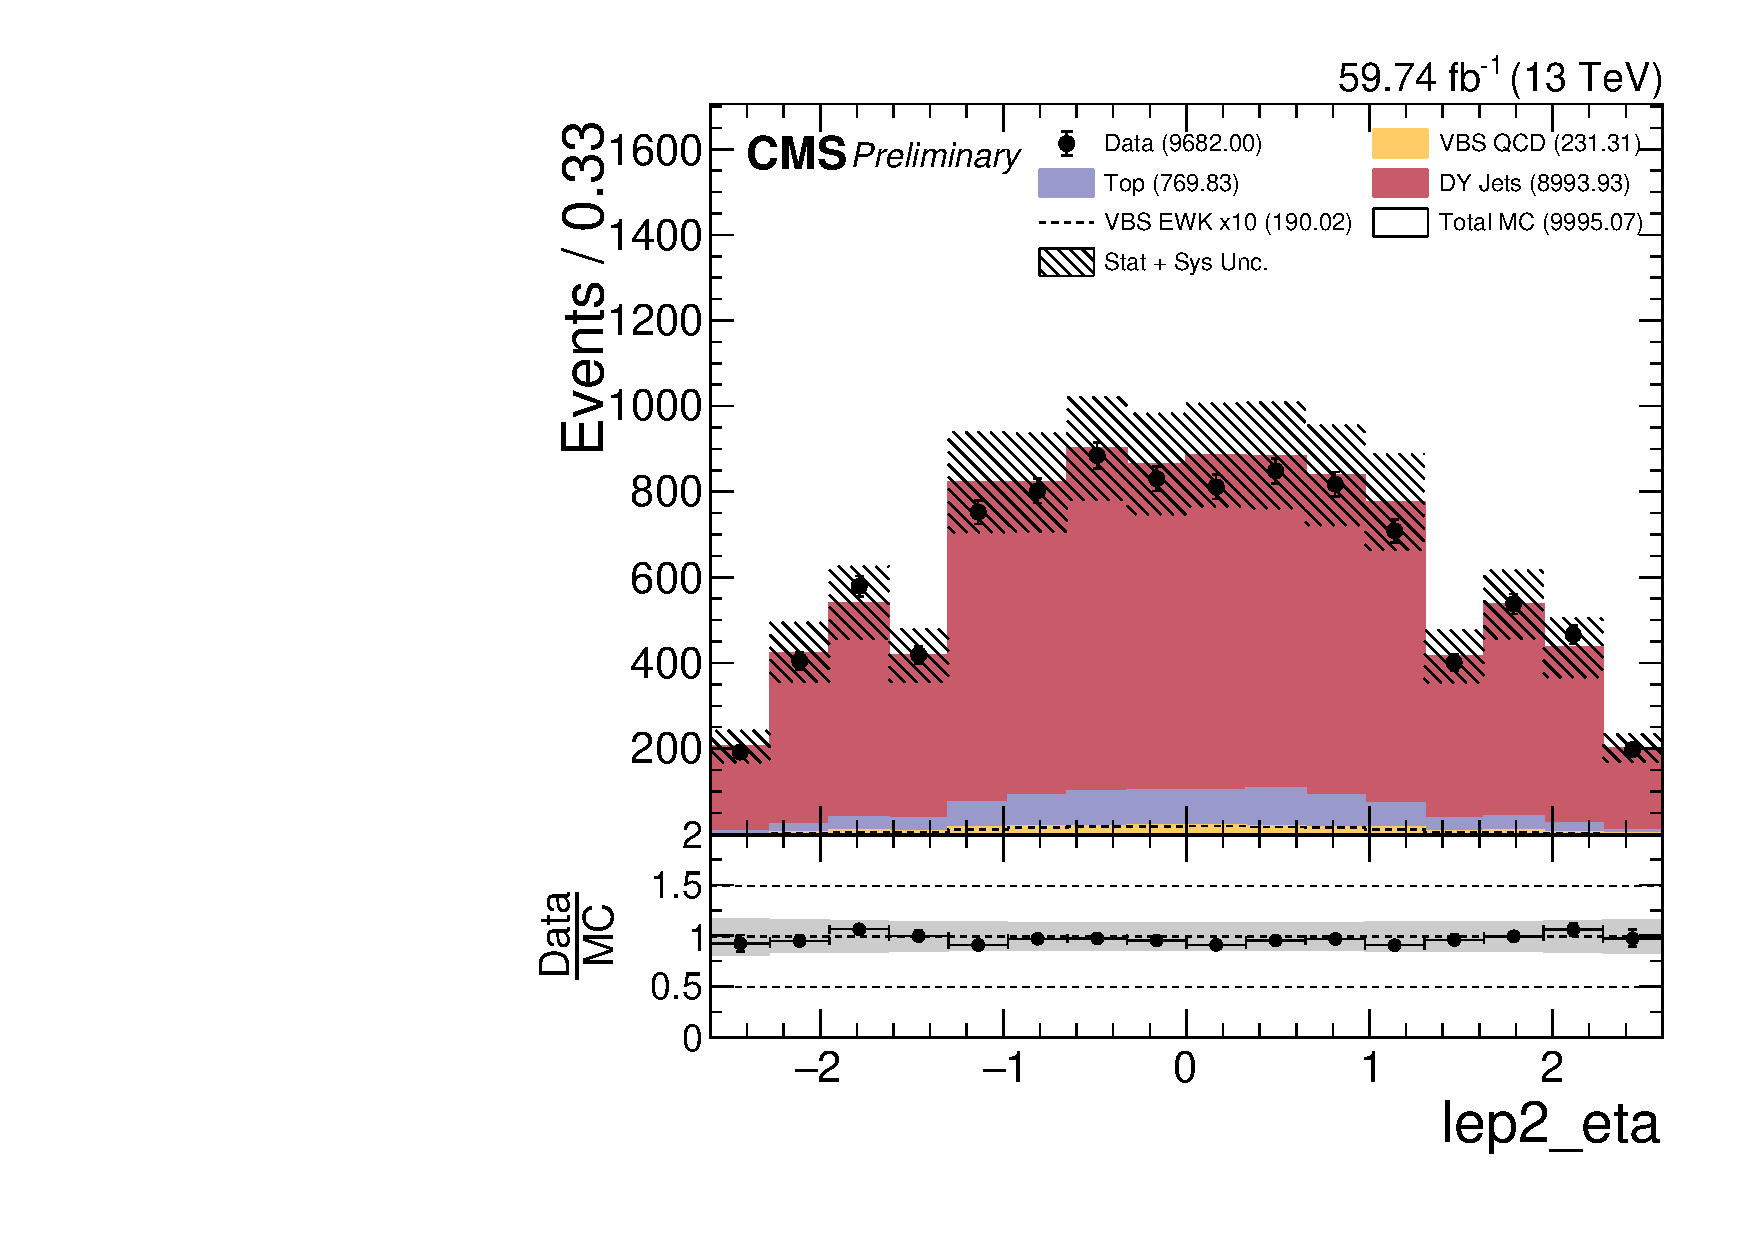
\includegraphics[width=0.335\textwidth]{analysis_plots/2018_zjj/cr_vjets_e/lep2_eta.pdf} \hspace{-10pt} \\
  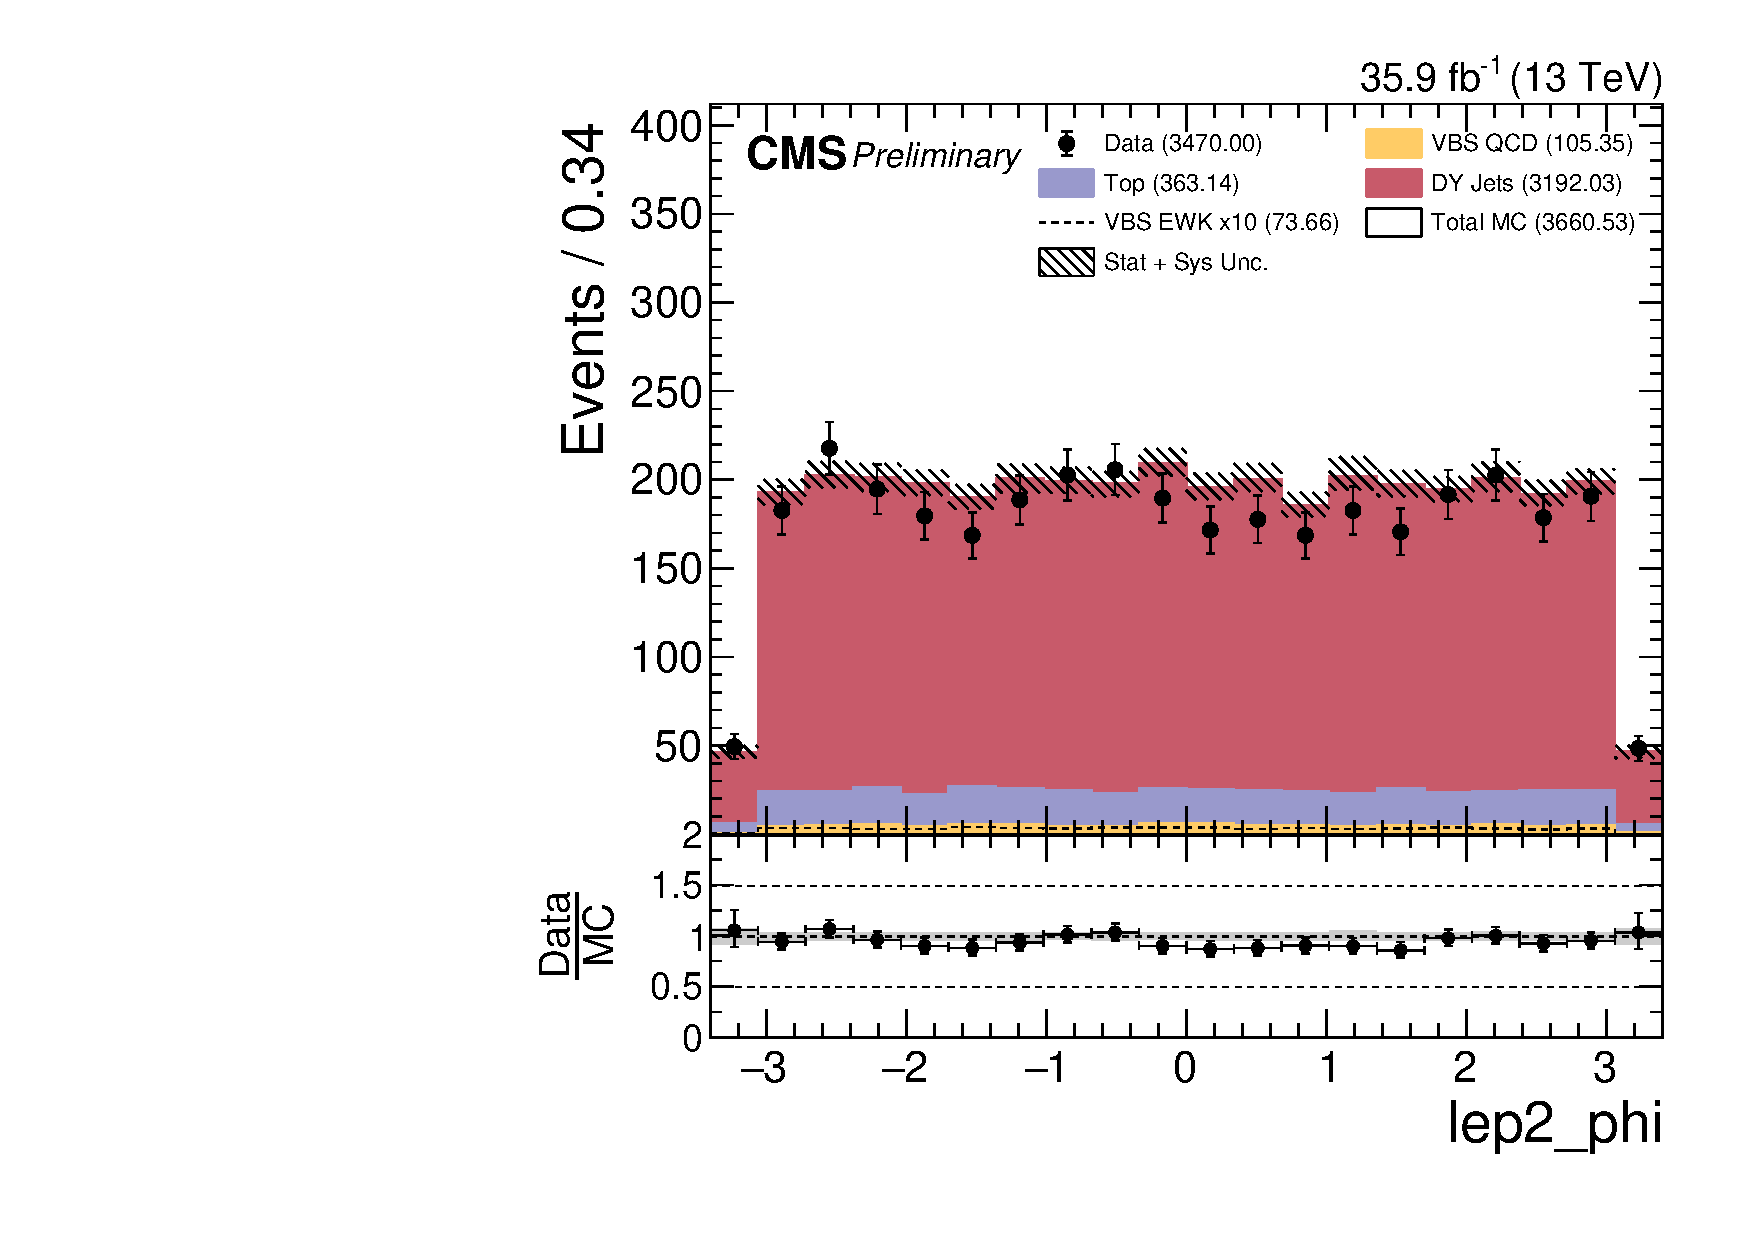
\includegraphics[width=0.335\textwidth]{analysis_plots/2016_zjj/cr_vjets_e/lep2_phi.pdf} \hspace{-10pt}
  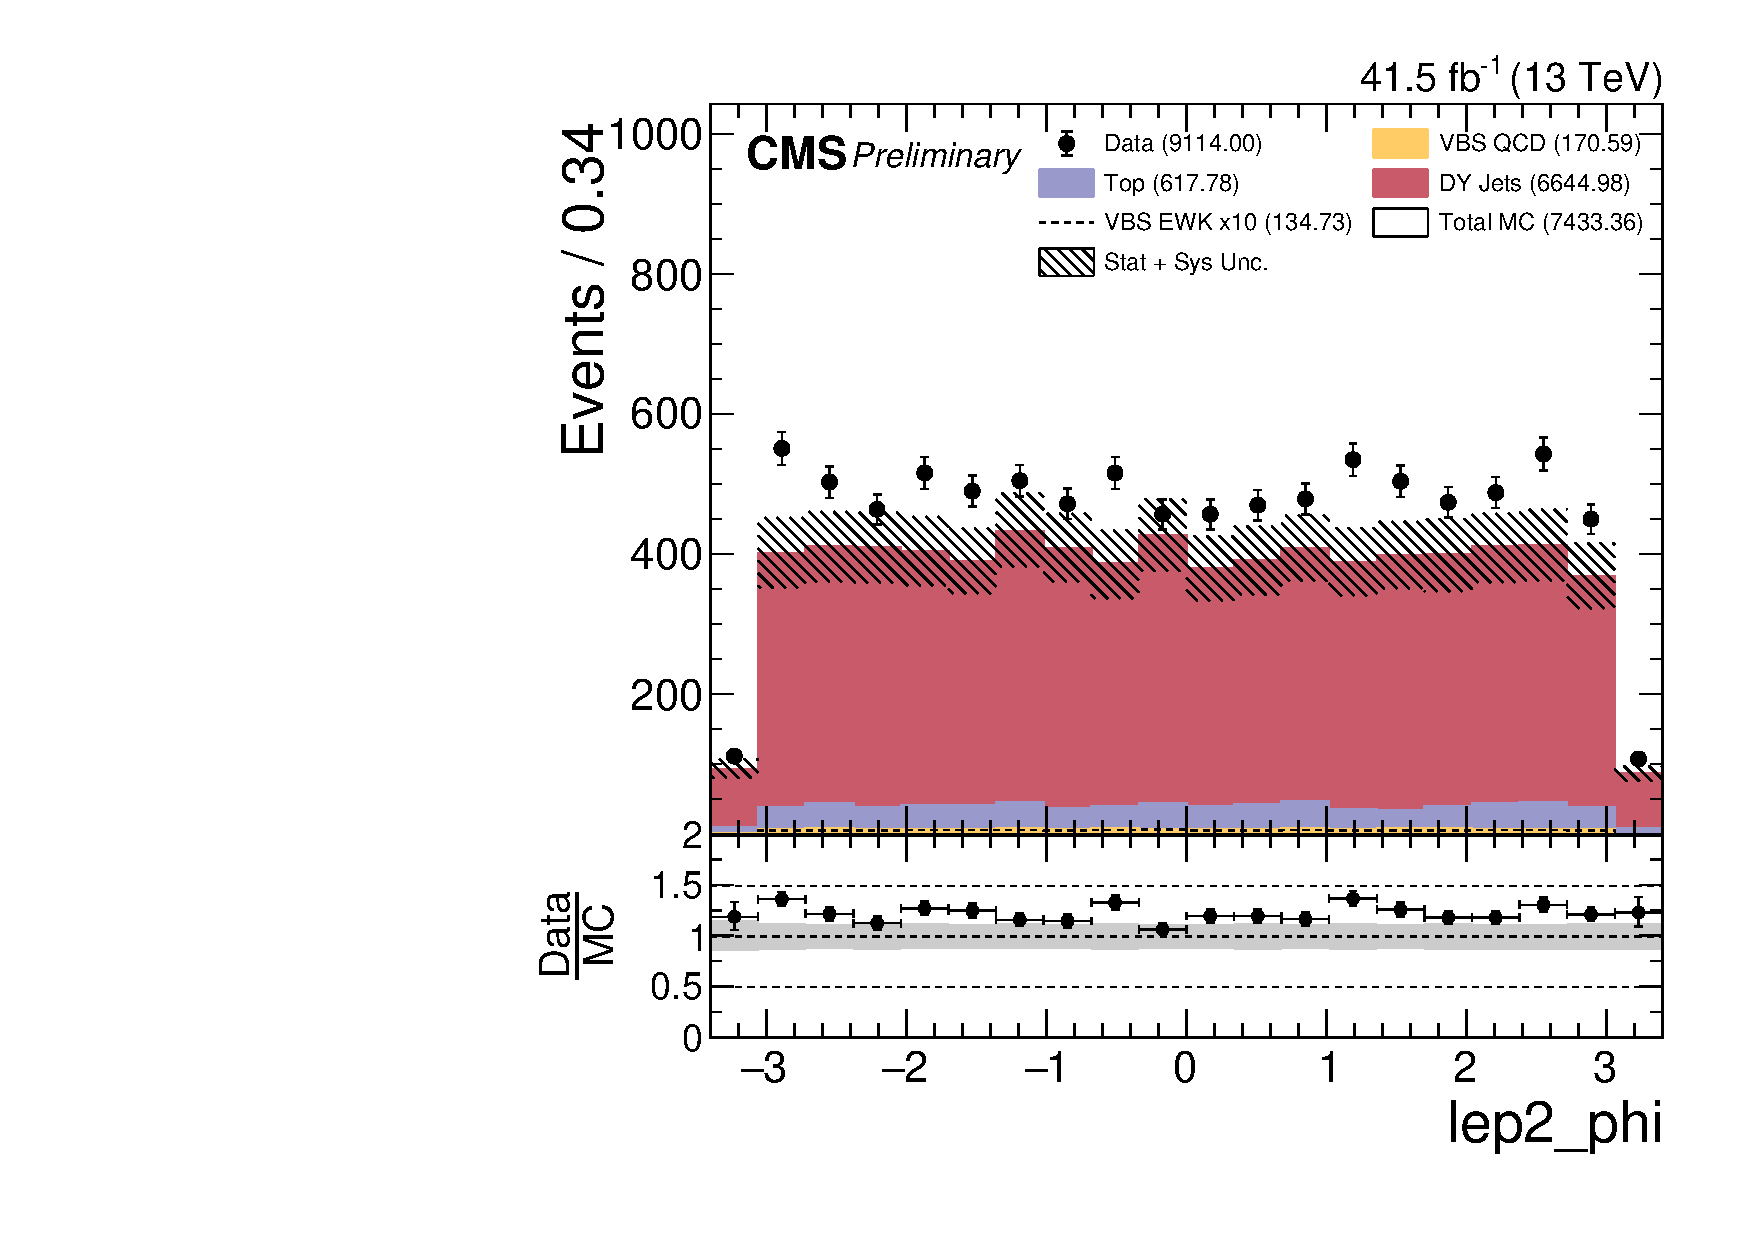
\includegraphics[width=0.335\textwidth]{analysis_plots/2017_zjj/cr_vjets_e/lep2_phi.pdf} \hspace{-10pt}
  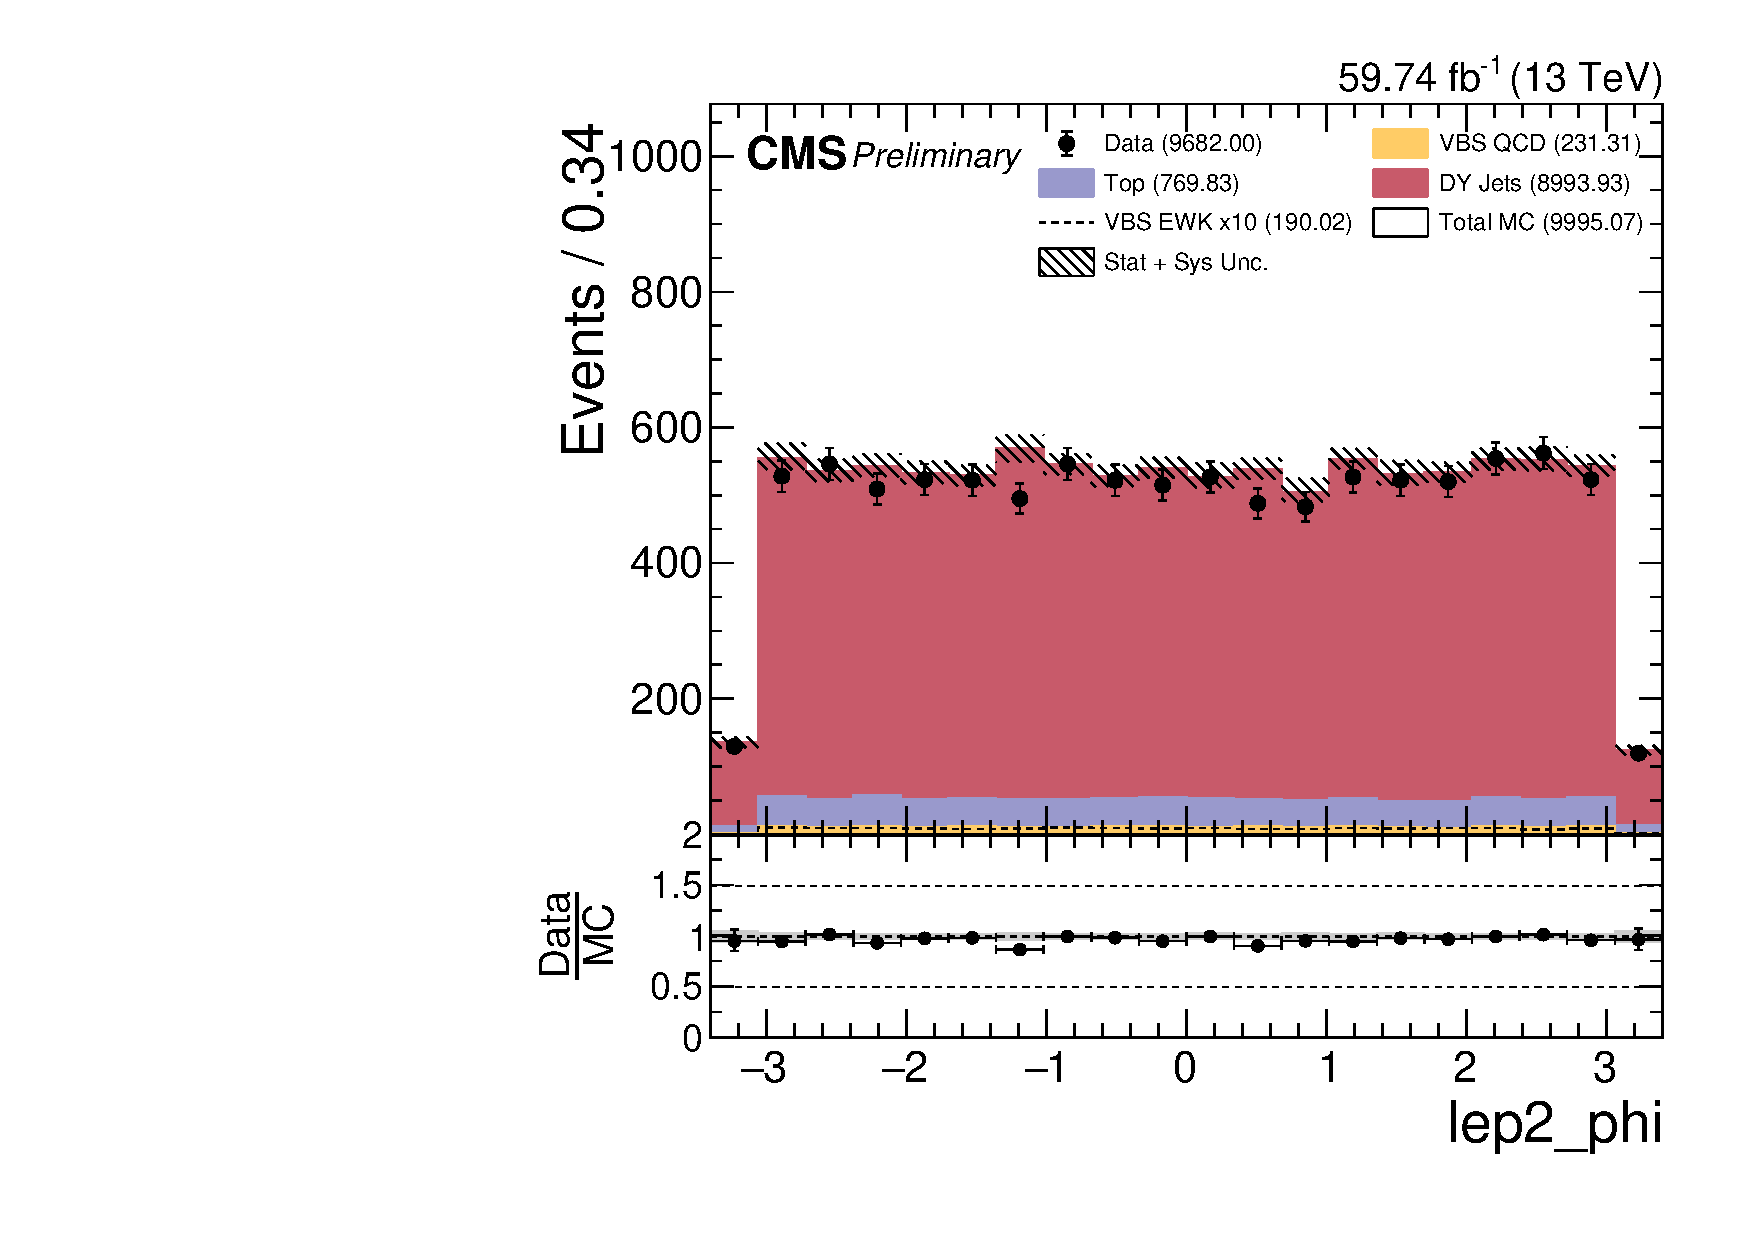
\includegraphics[width=0.335\textwidth]{analysis_plots/2018_zjj/cr_vjets_e/lep2_phi.pdf} \hspace{-10pt} \\
  \caption[DY+Jets Control Region: Trailing electron kinematics in Resolved ZV Channel]%
  {DY+Jets Control Region: Trailing electron kinematics in Resolved ZV Channel.
    Error bars include statistical uncertainty on total background,
    JES and QCD scale systematic on DY+Jets and VBS\_QCD MC\@. From Left to Right: 2016,
    2017, and 2018. From Top to Bottom: \( p_T \), \( \eta \), and \( \phi \).}%
  \label{fig:zjj-cr-vjets-e-lep2-pt-eta-phi}
\end{figure}

\begin{figure}[!ht]
  \centering
  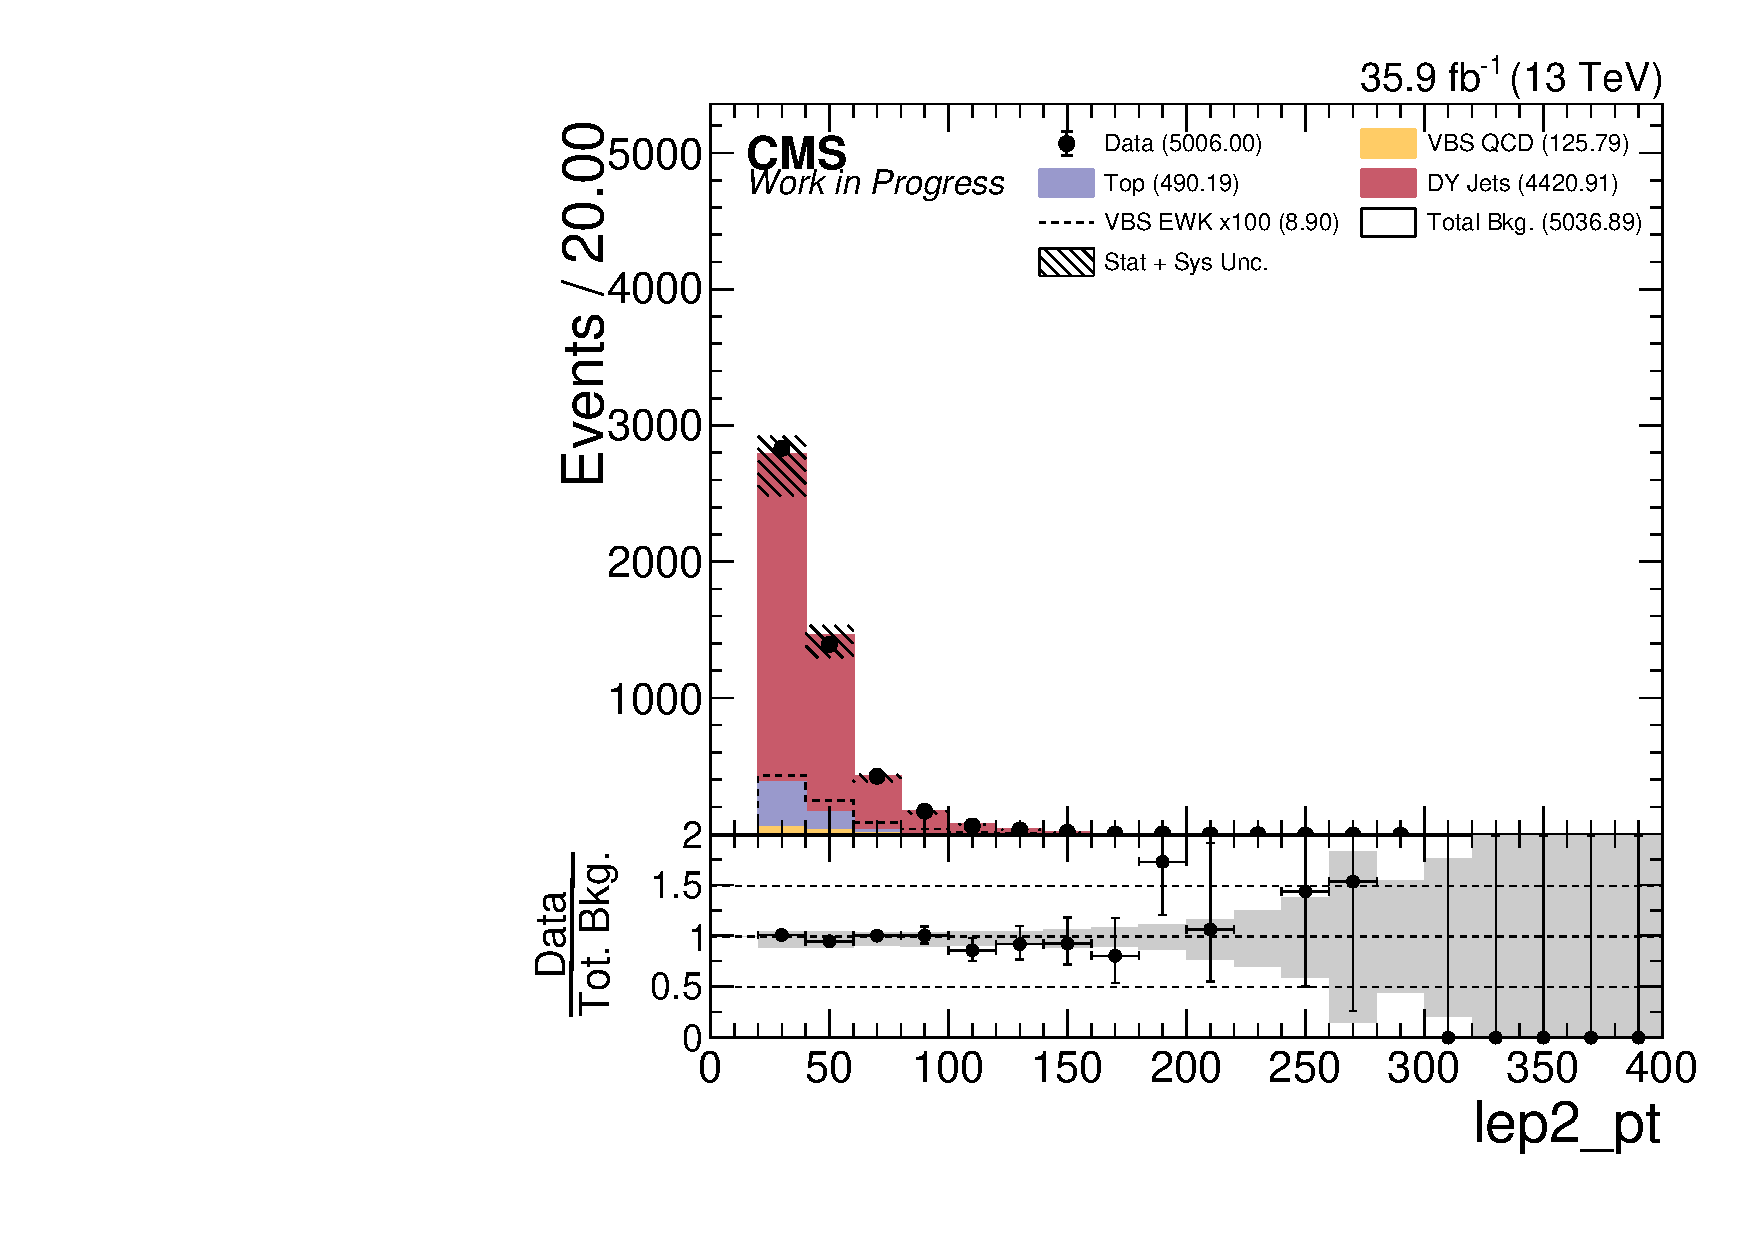
\includegraphics[width=0.335\textwidth]{analysis_plots/2016_zjj/cr_vjets_m/lep2_pt.pdf} \hspace{-10pt}
  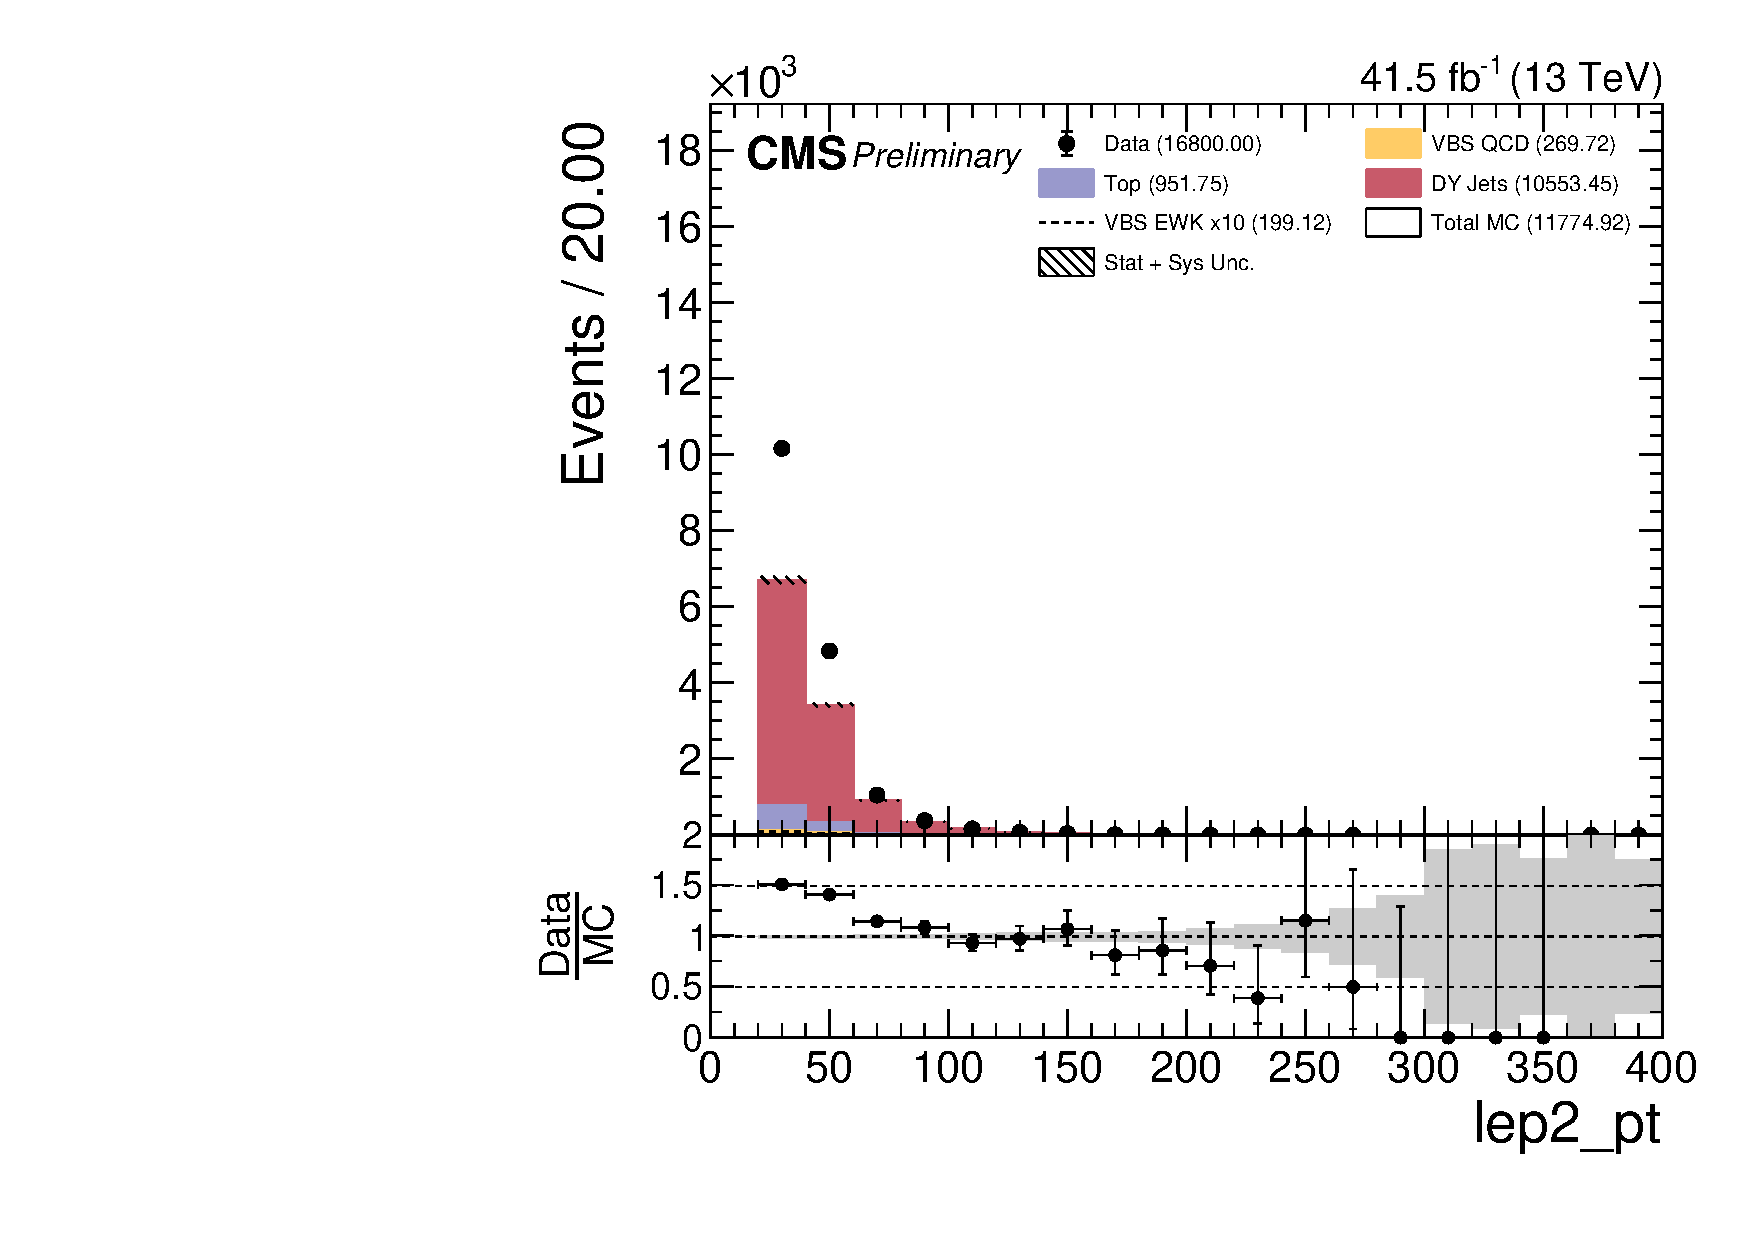
\includegraphics[width=0.335\textwidth]{analysis_plots/2017_zjj/cr_vjets_m/lep2_pt.pdf} \hspace{-10pt}
  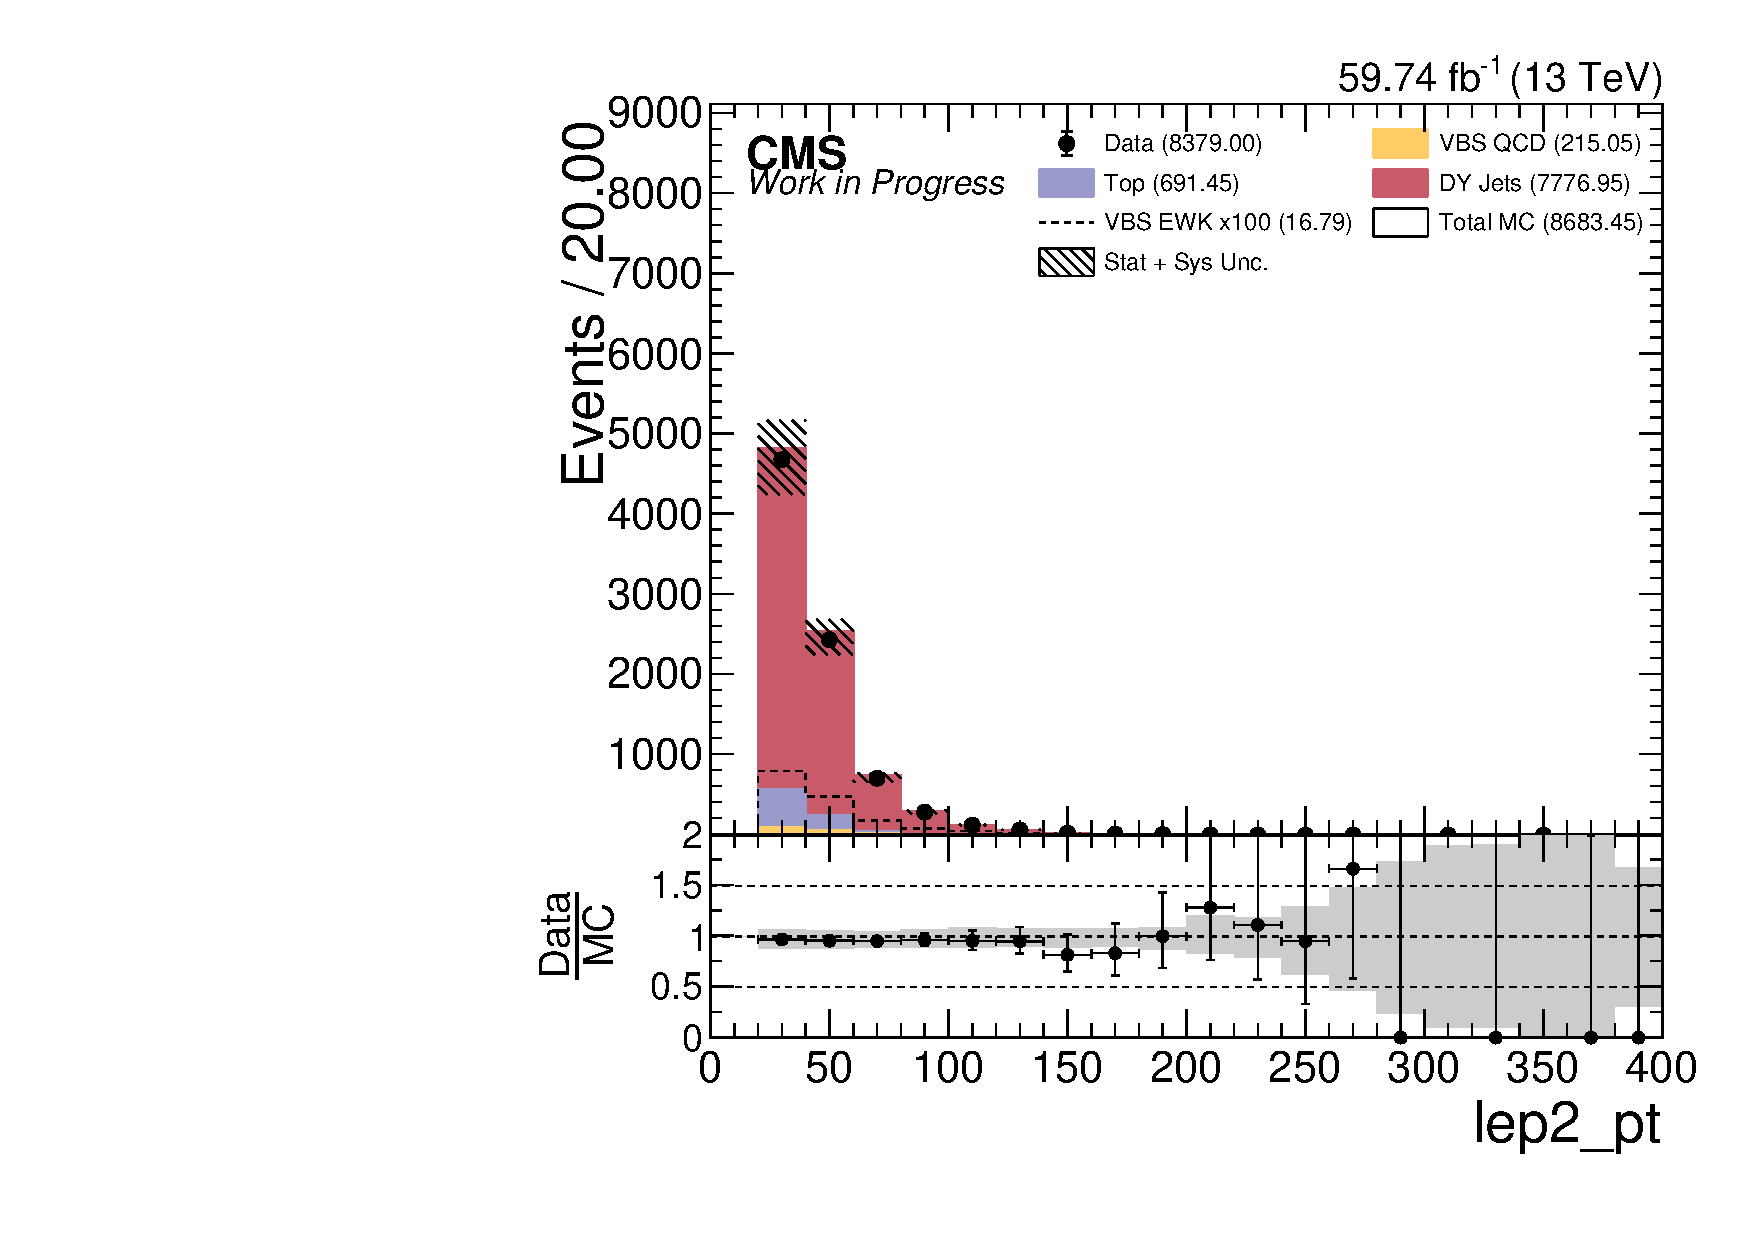
\includegraphics[width=0.335\textwidth]{analysis_plots/2018_zjj/cr_vjets_m/lep2_pt.pdf} \hspace{-10pt} \\
  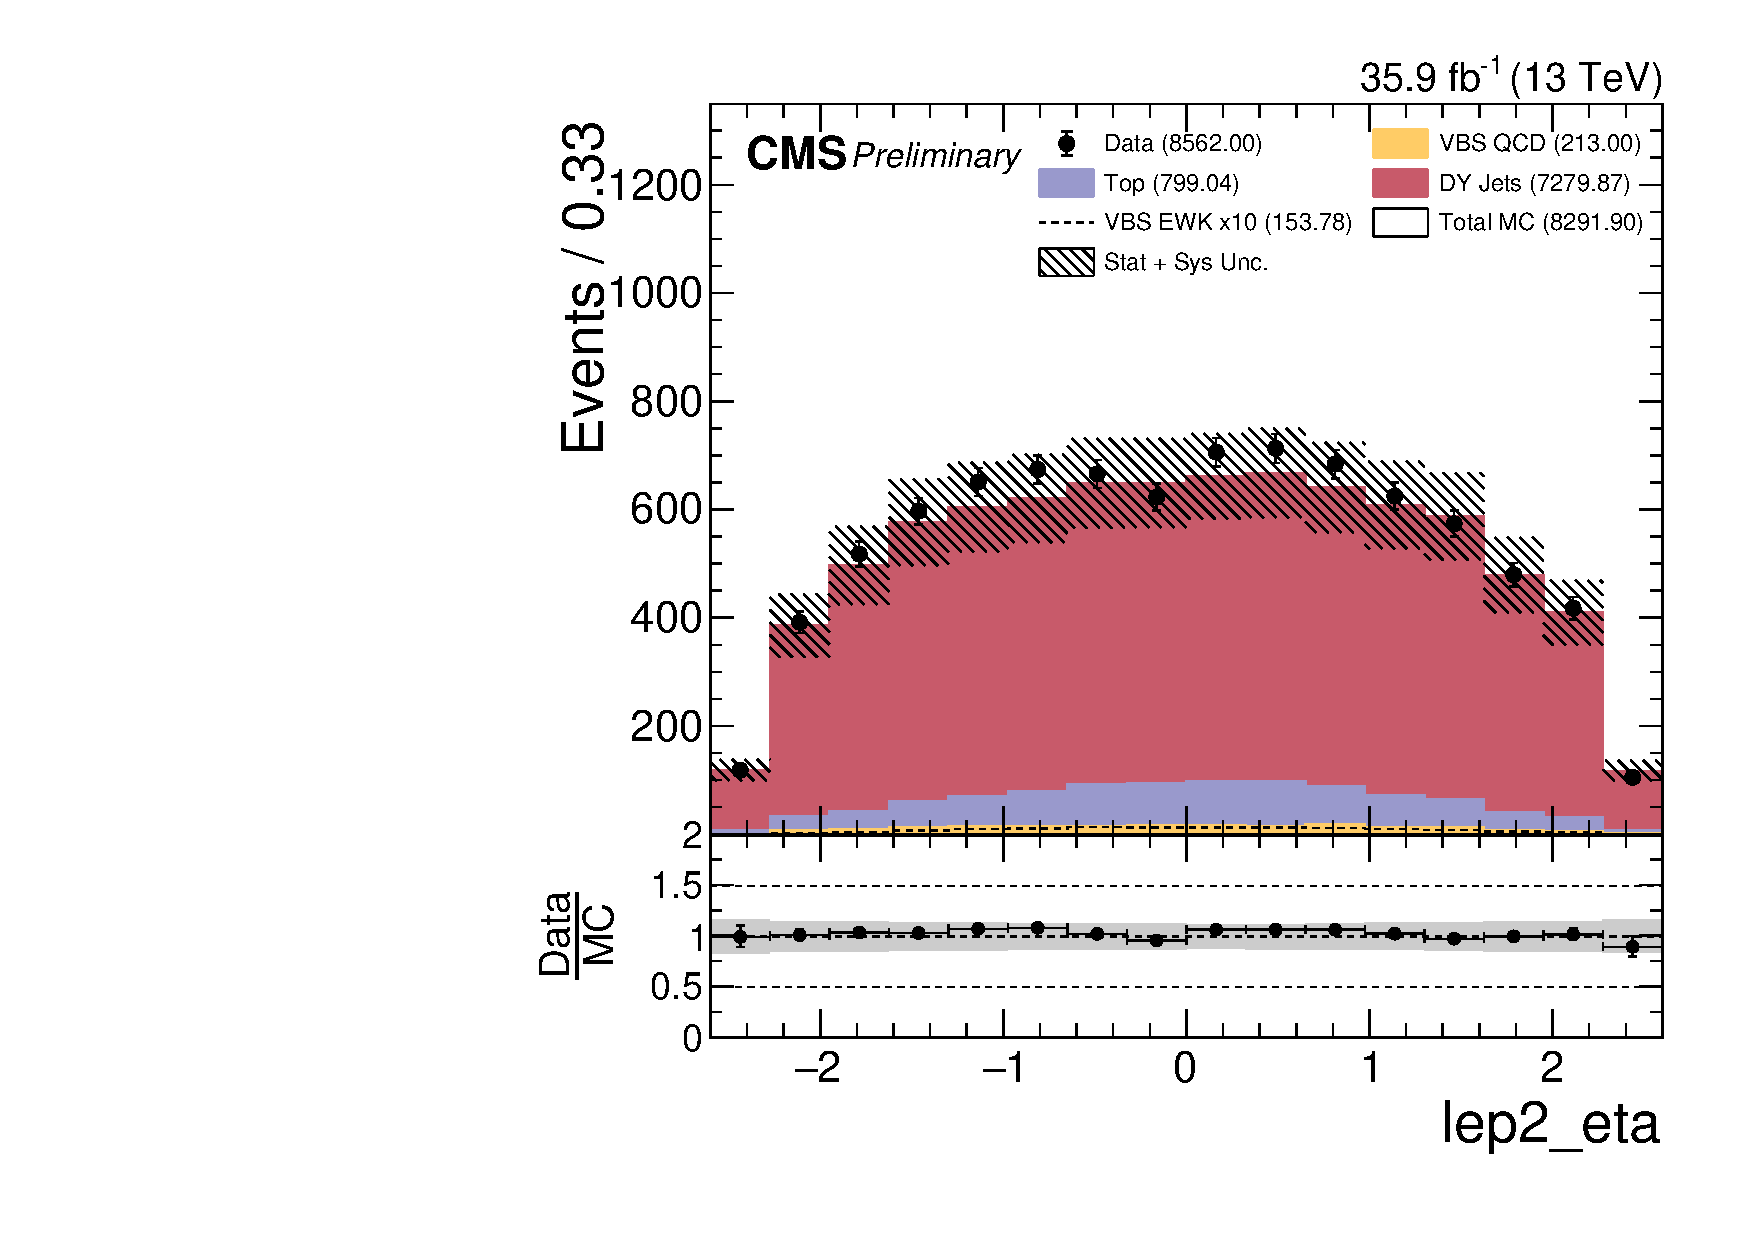
\includegraphics[width=0.335\textwidth]{analysis_plots/2016_zjj/cr_vjets_m/lep2_eta.pdf} \hspace{-10pt}
  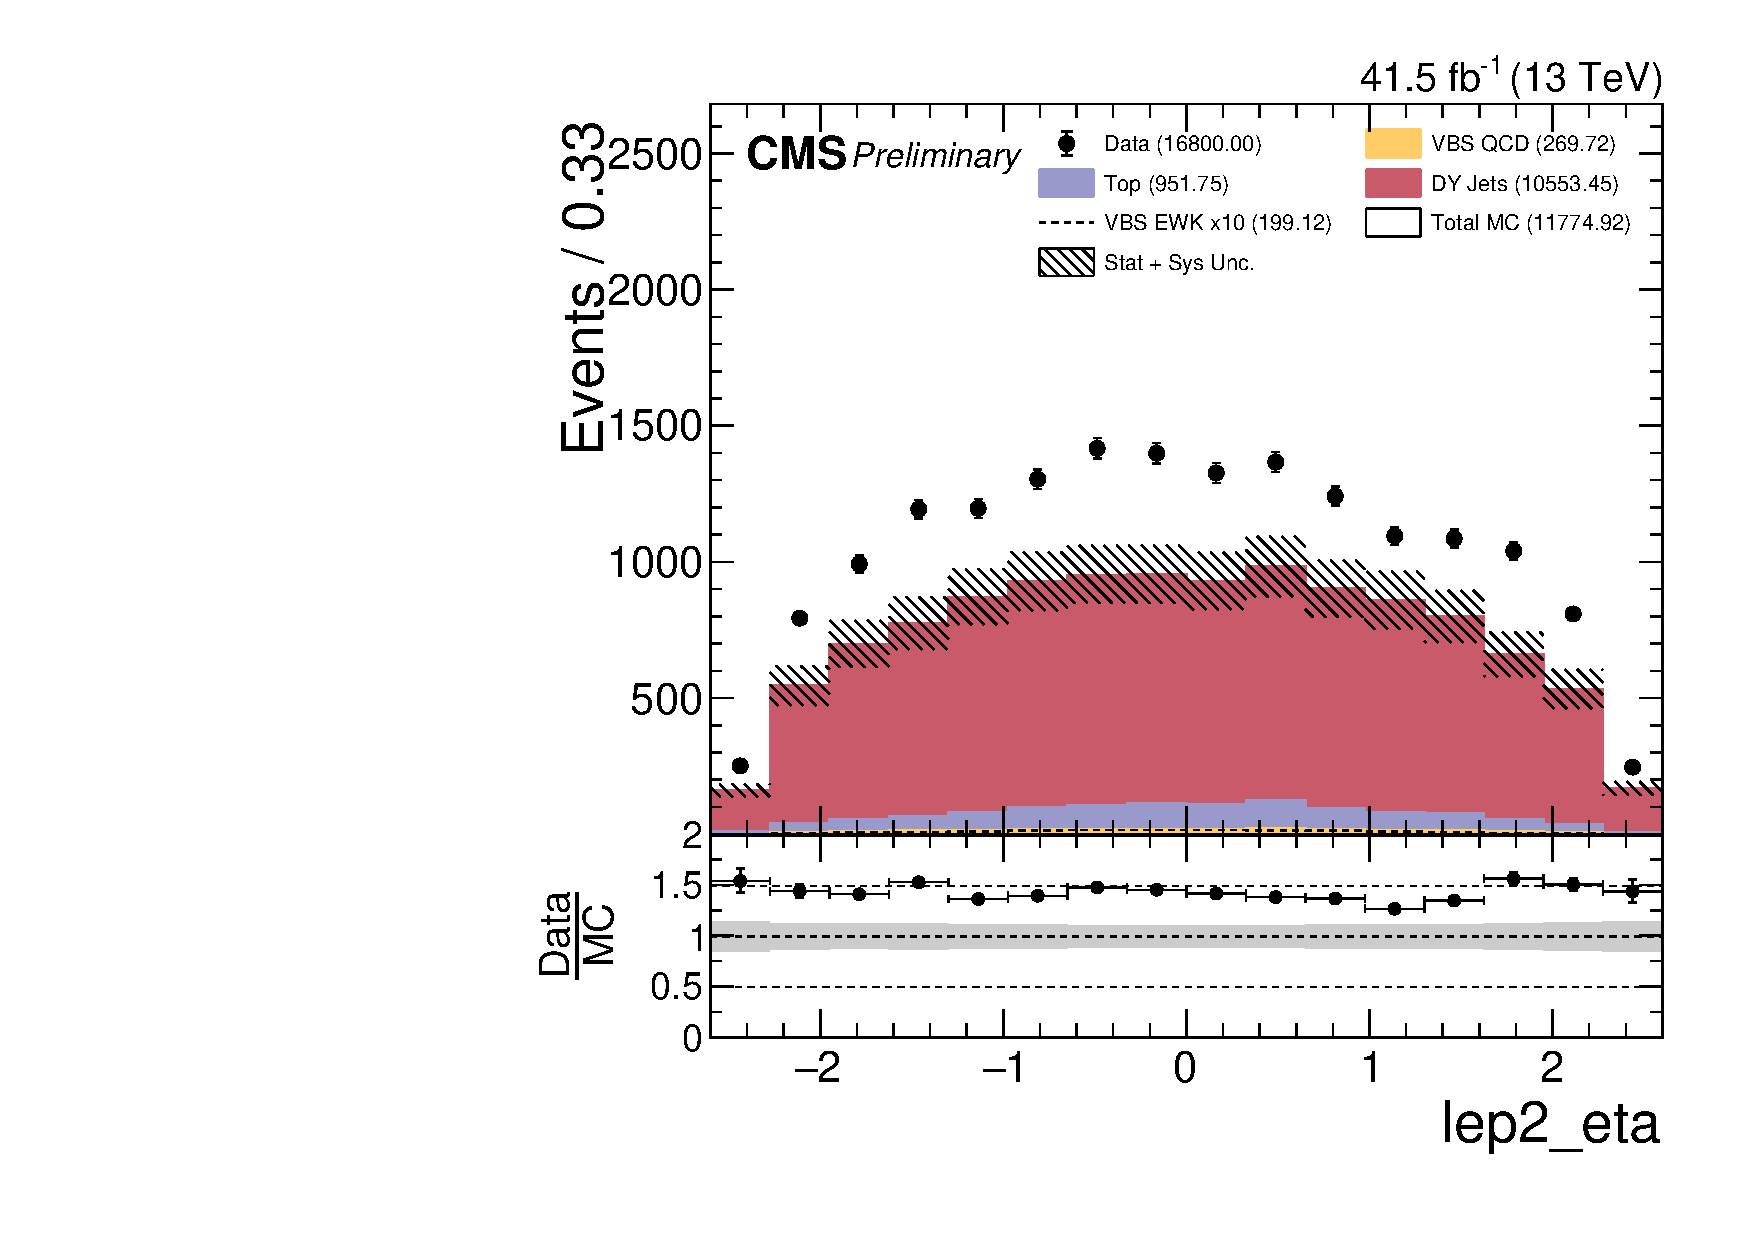
\includegraphics[width=0.335\textwidth]{analysis_plots/2017_zjj/cr_vjets_m/lep2_eta.pdf} \hspace{-10pt}
  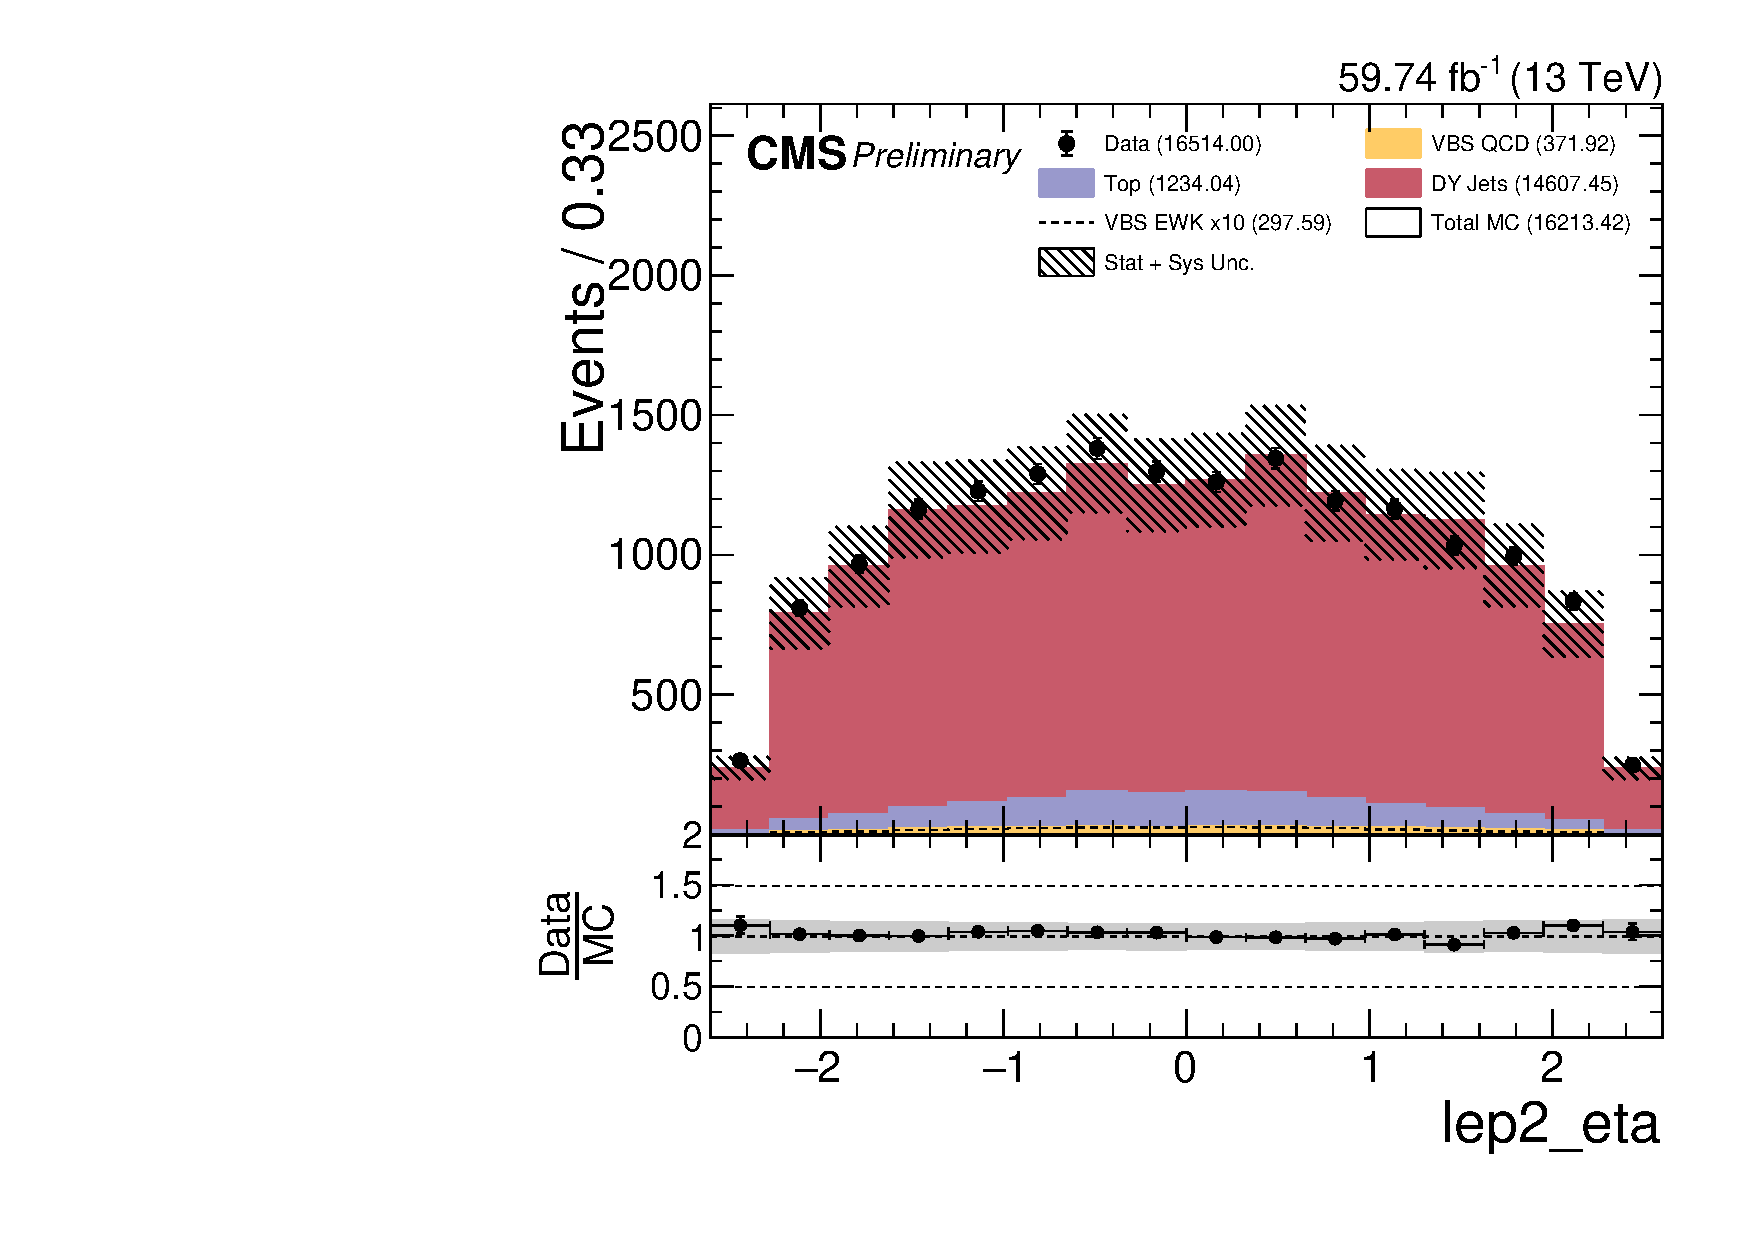
\includegraphics[width=0.335\textwidth]{analysis_plots/2018_zjj/cr_vjets_m/lep2_eta.pdf} \hspace{-10pt} \\
  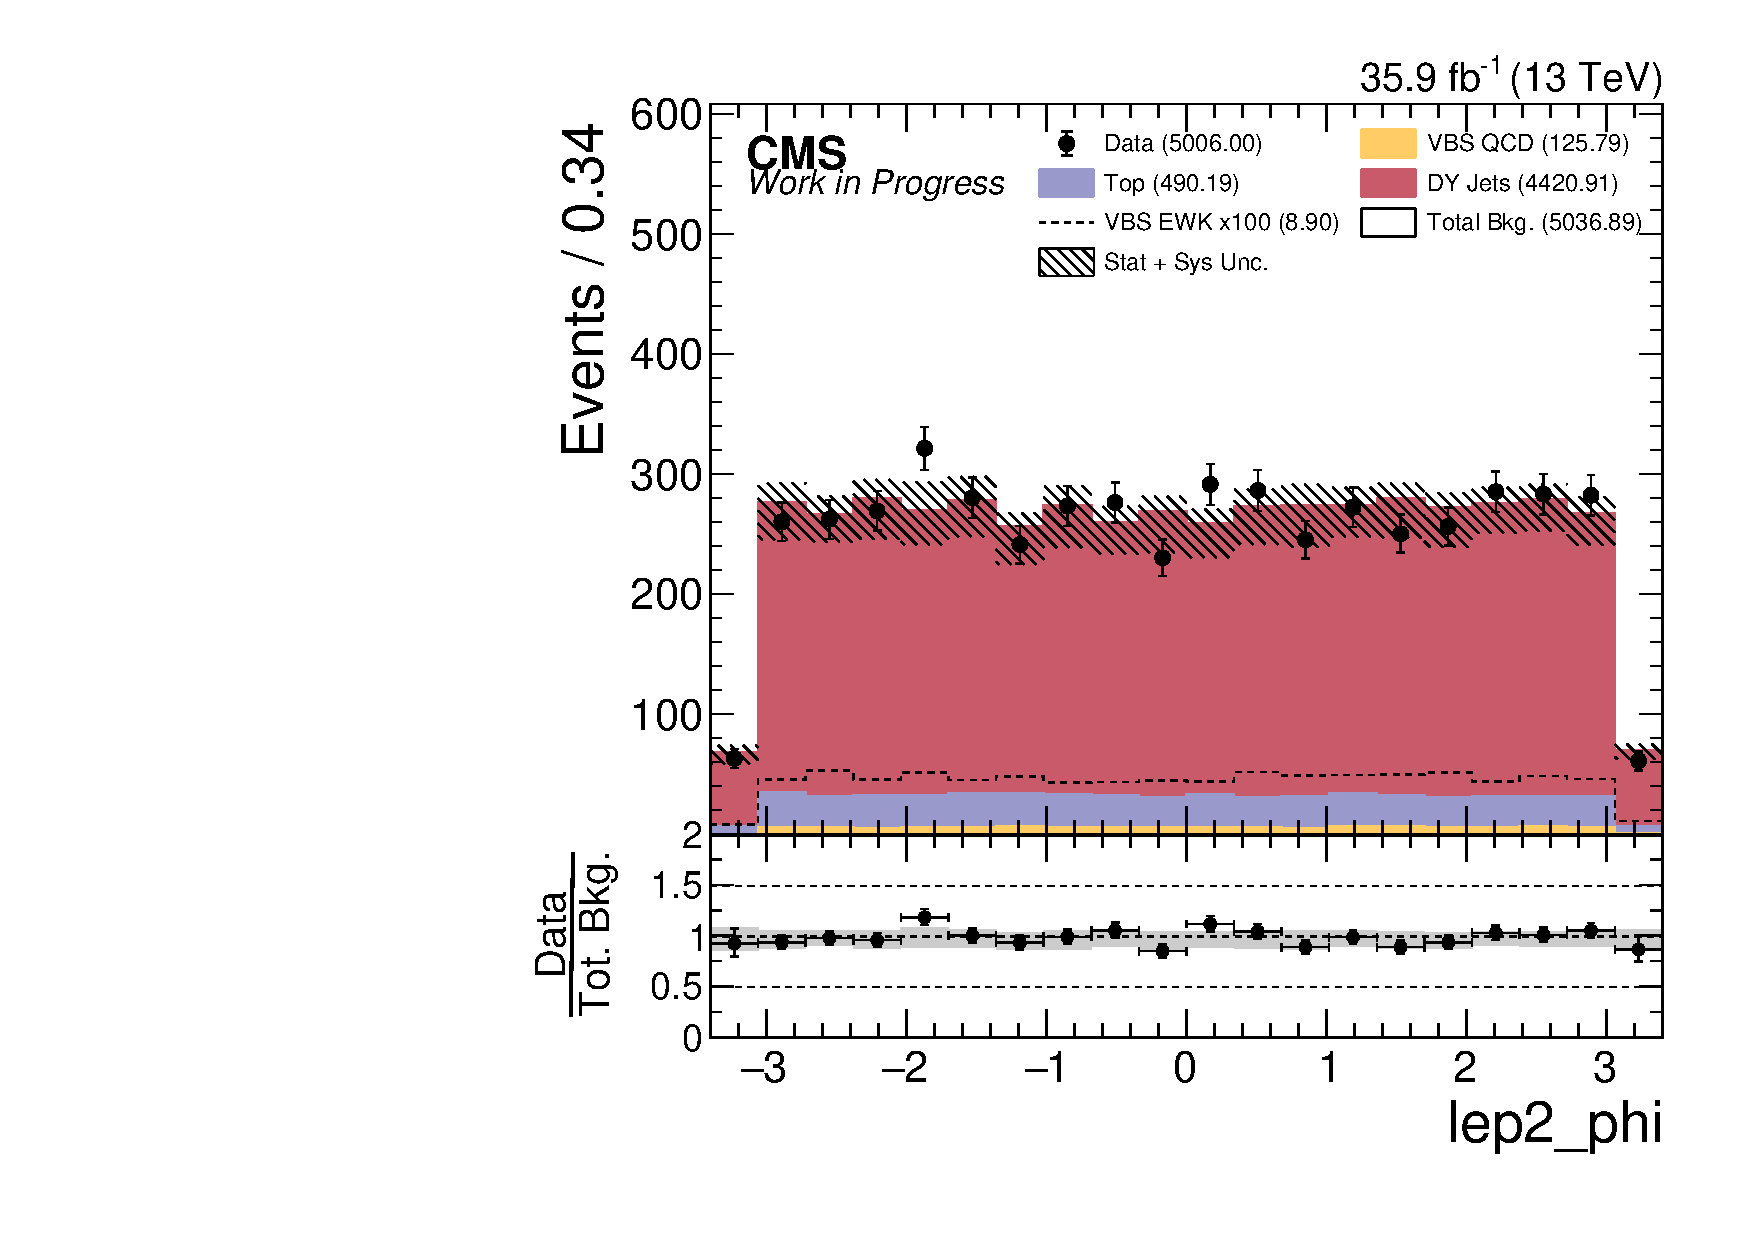
\includegraphics[width=0.335\textwidth]{analysis_plots/2016_zjj/cr_vjets_m/lep2_phi.pdf} \hspace{-10pt}
  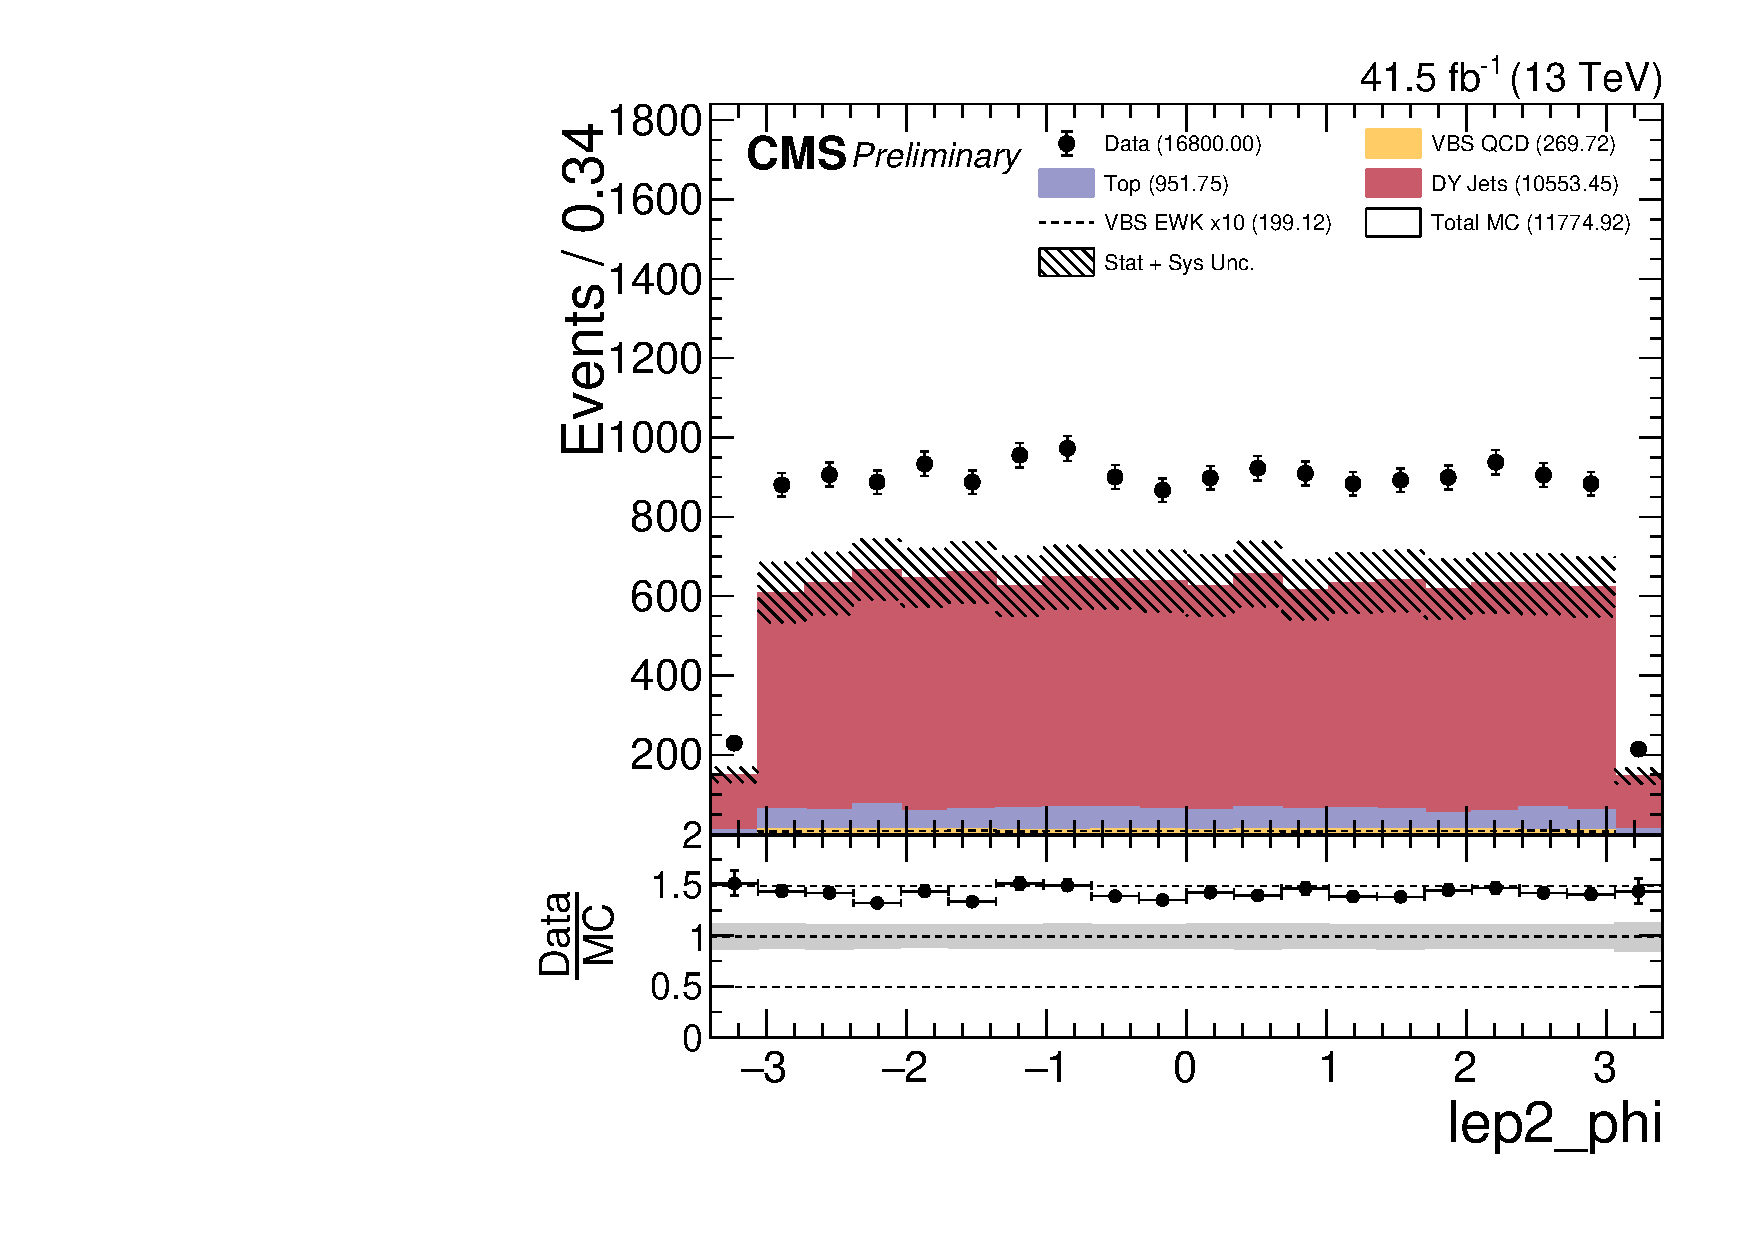
\includegraphics[width=0.335\textwidth]{analysis_plots/2017_zjj/cr_vjets_m/lep2_phi.pdf} \hspace{-10pt}
  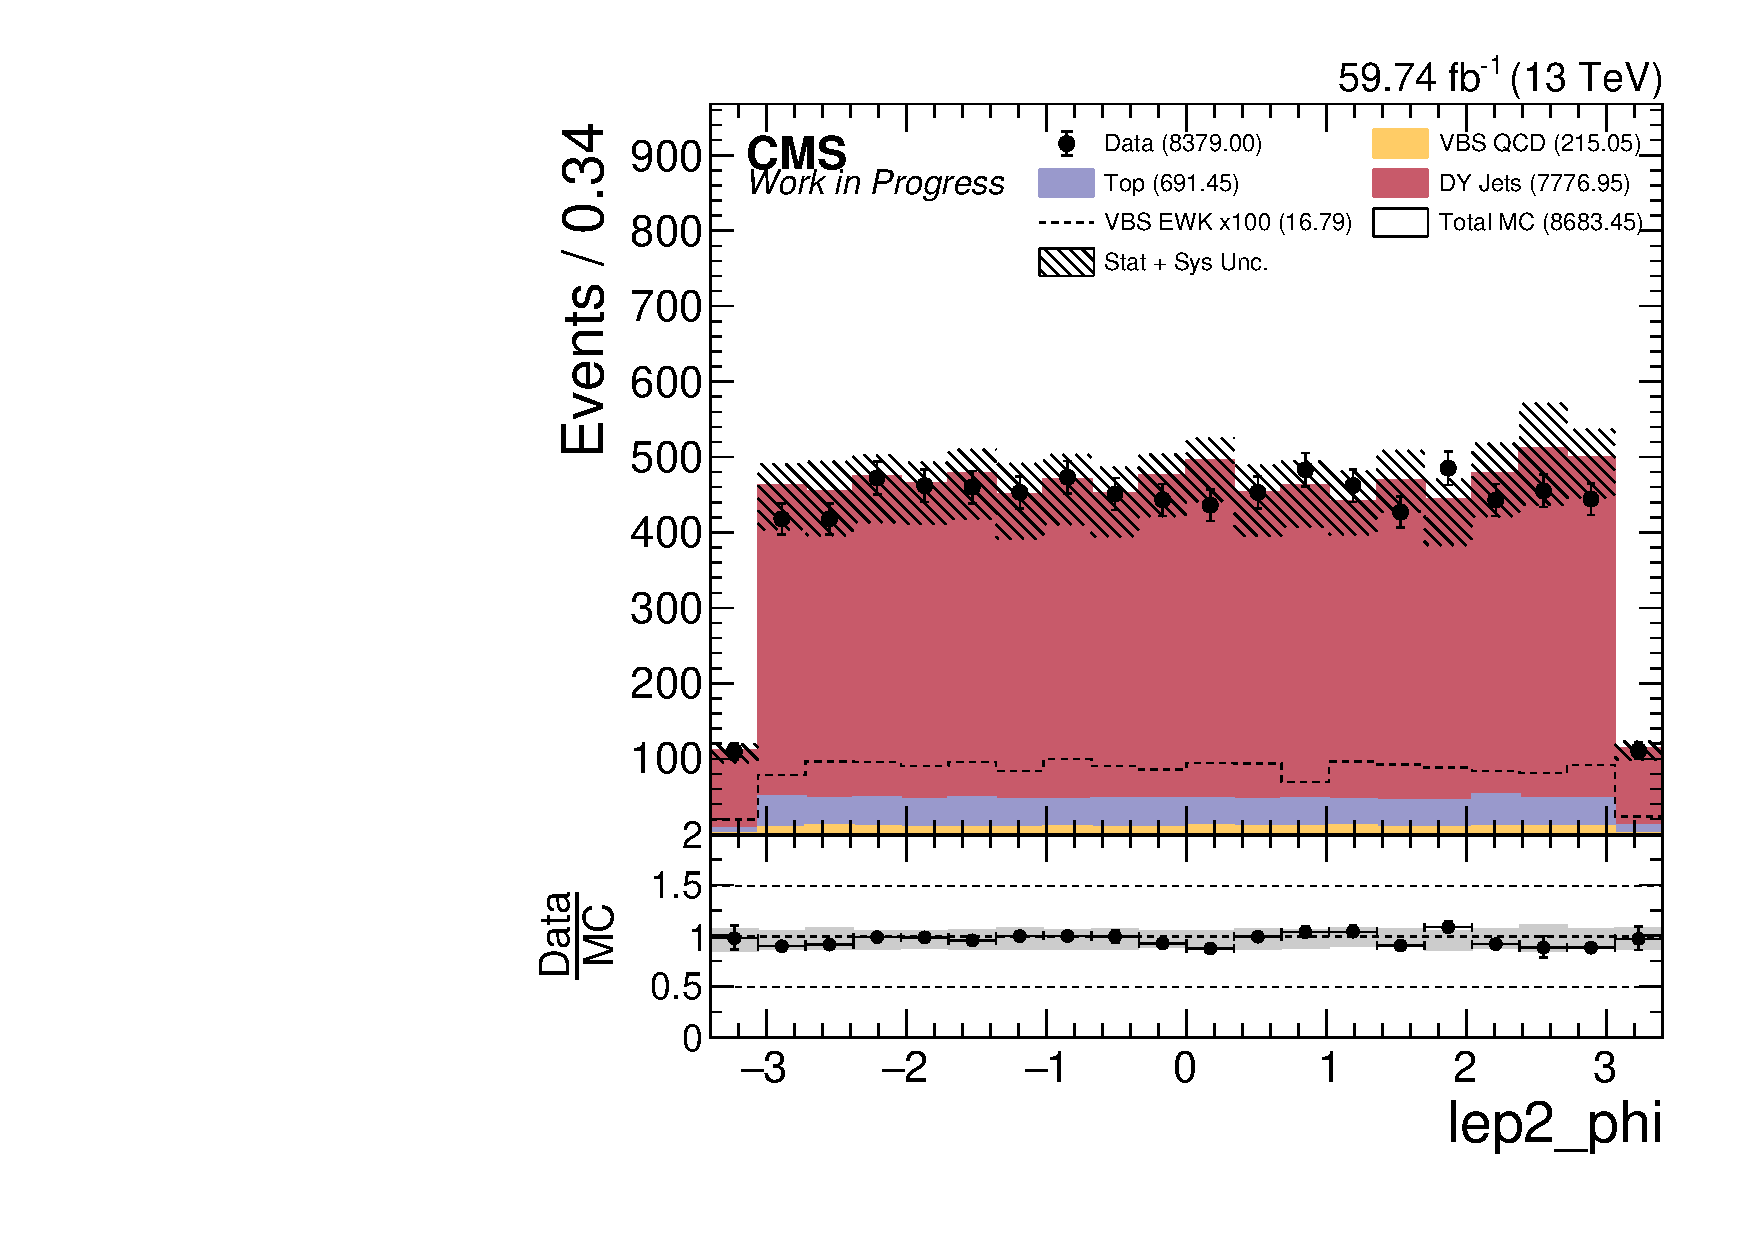
\includegraphics[width=0.335\textwidth]{analysis_plots/2018_zjj/cr_vjets_m/lep2_phi.pdf} \hspace{-10pt} \\
  \caption[DY+Jets Control Region: Trailing muon kinematics in Resolved ZV Channel]%
  {DY+Jets Control Region: Trailing muon kinematics in Resolved ZV Channel.
    Error bars include statistical uncertainty on total background,
    JES and QCD scale systematic on DY+Jets and VBS\_QCD MC\@. From Left to Right: 2016,
    2017, and 2018. From Top to Bottom: \( p_T \), \( \eta \), and \( \phi \).}%
  \label{fig:zjj-cr-vjets-m-lep2-pt-eta-phi}
\end{figure}

\begin{figure}[!ht]
  \centering
  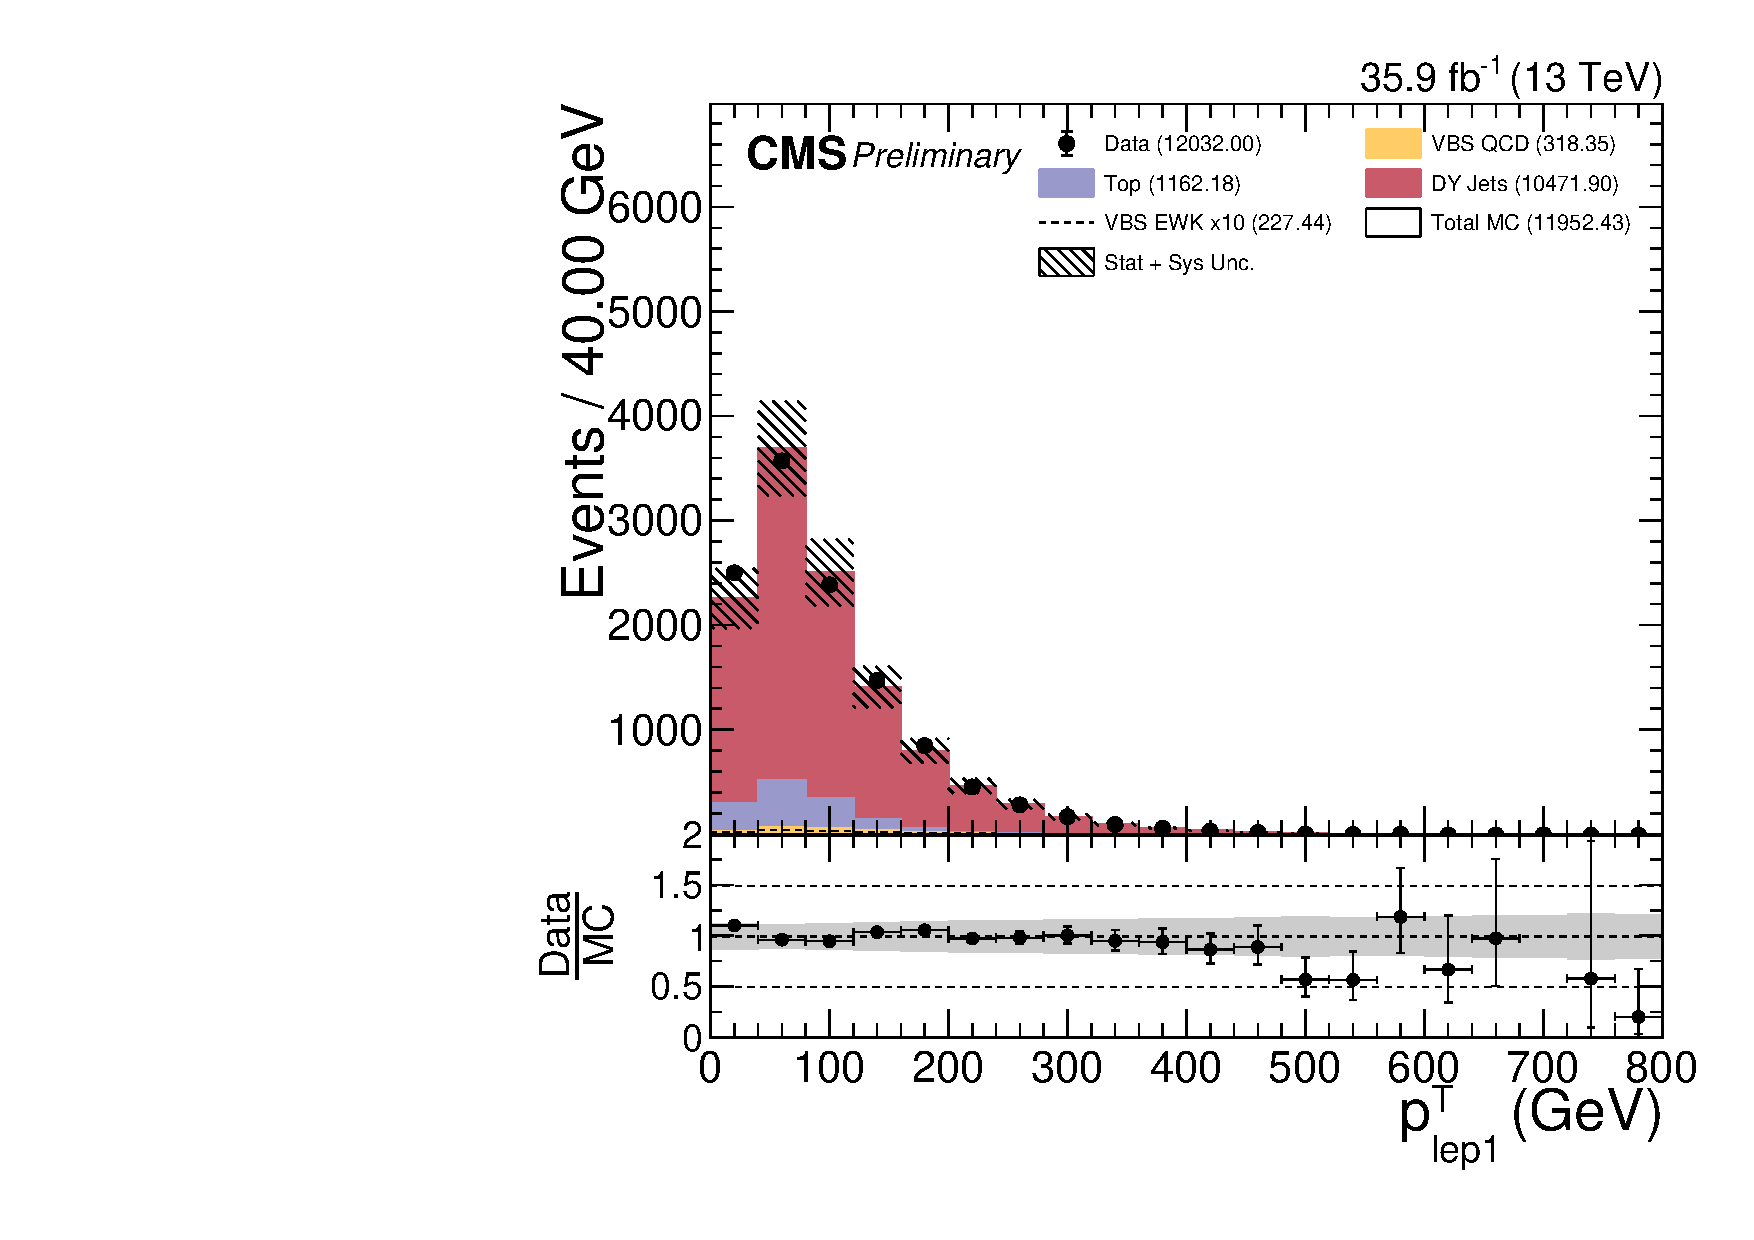
\includegraphics[width=0.335\textwidth]{analysis_plots/2016_zjj/cr_vjets_l/v_lep_pt.pdf} \hspace{-10pt}
  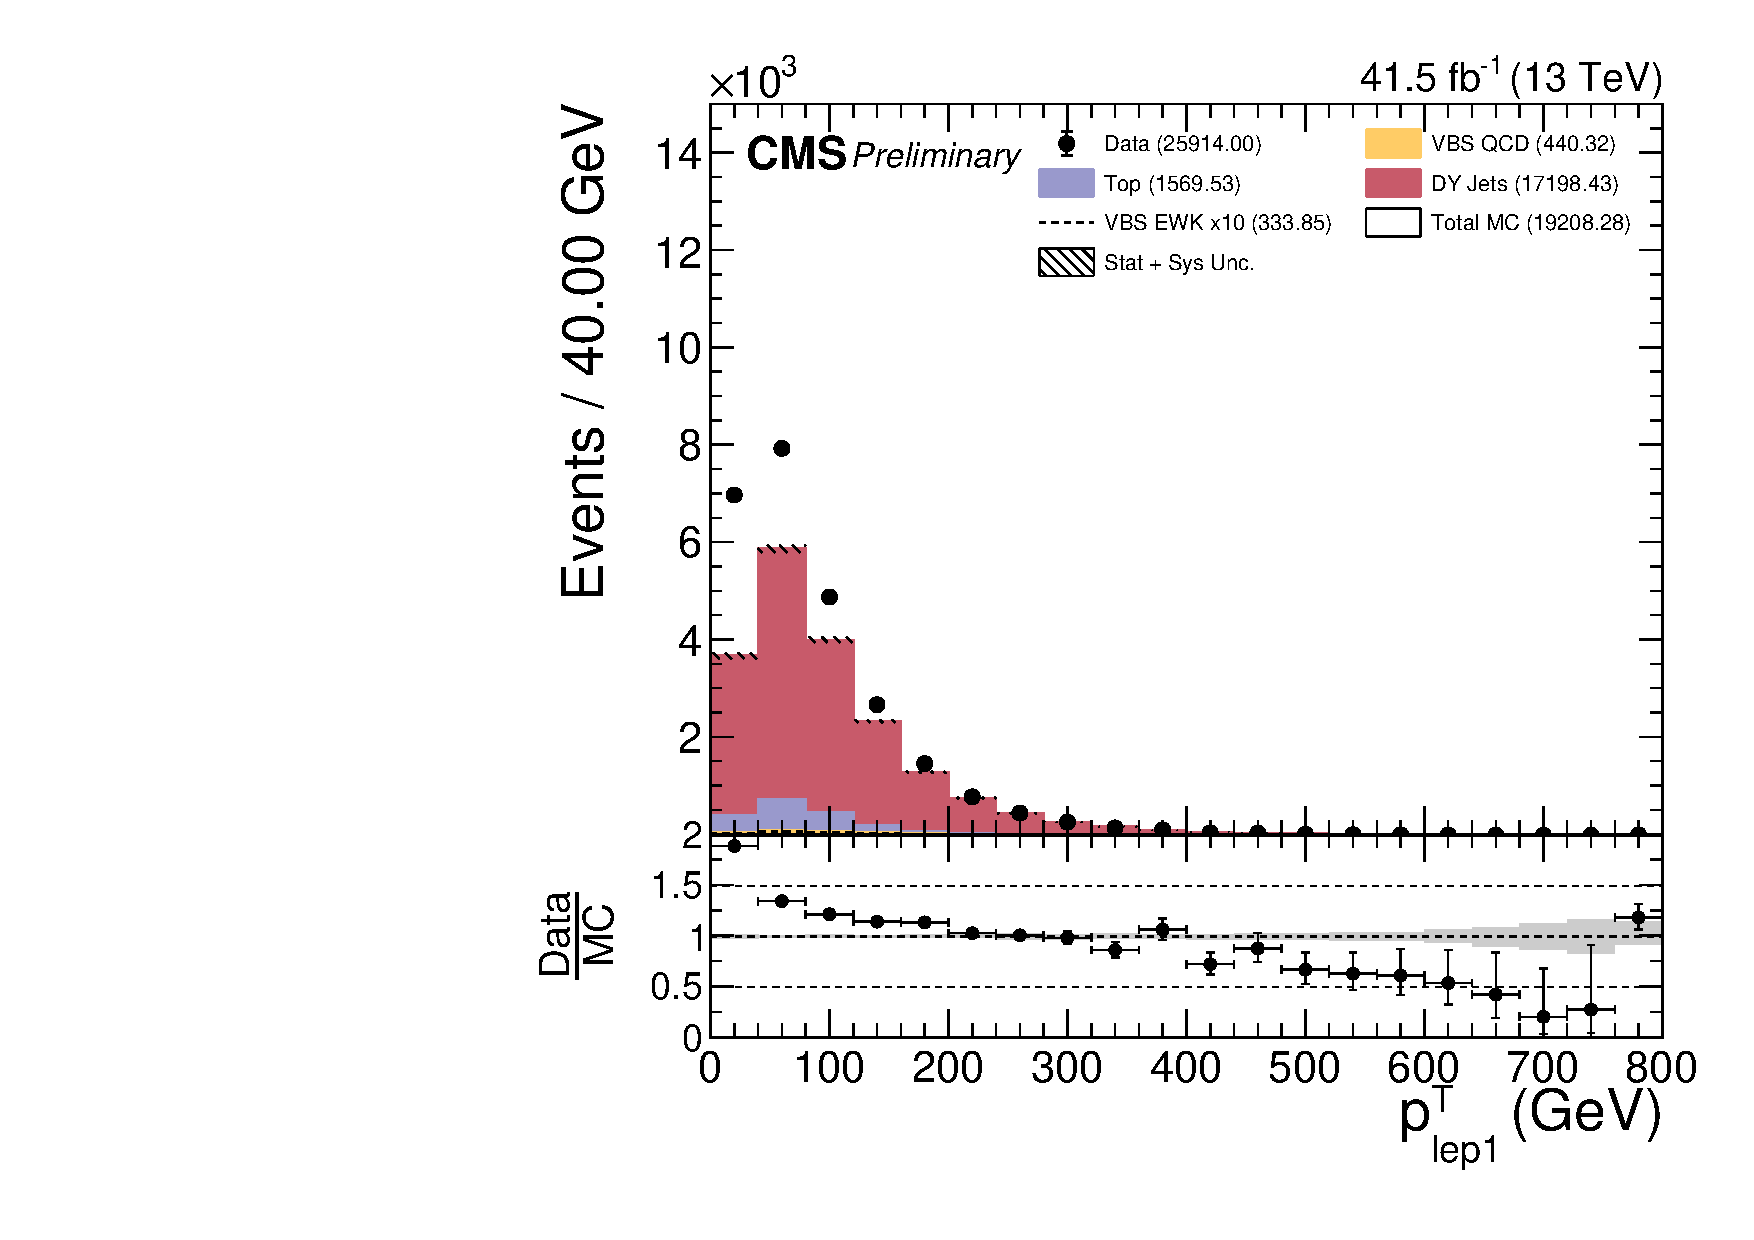
\includegraphics[width=0.335\textwidth]{analysis_plots/2017_zjj/cr_vjets_l/v_lep_pt.pdf} \hspace{-10pt}
  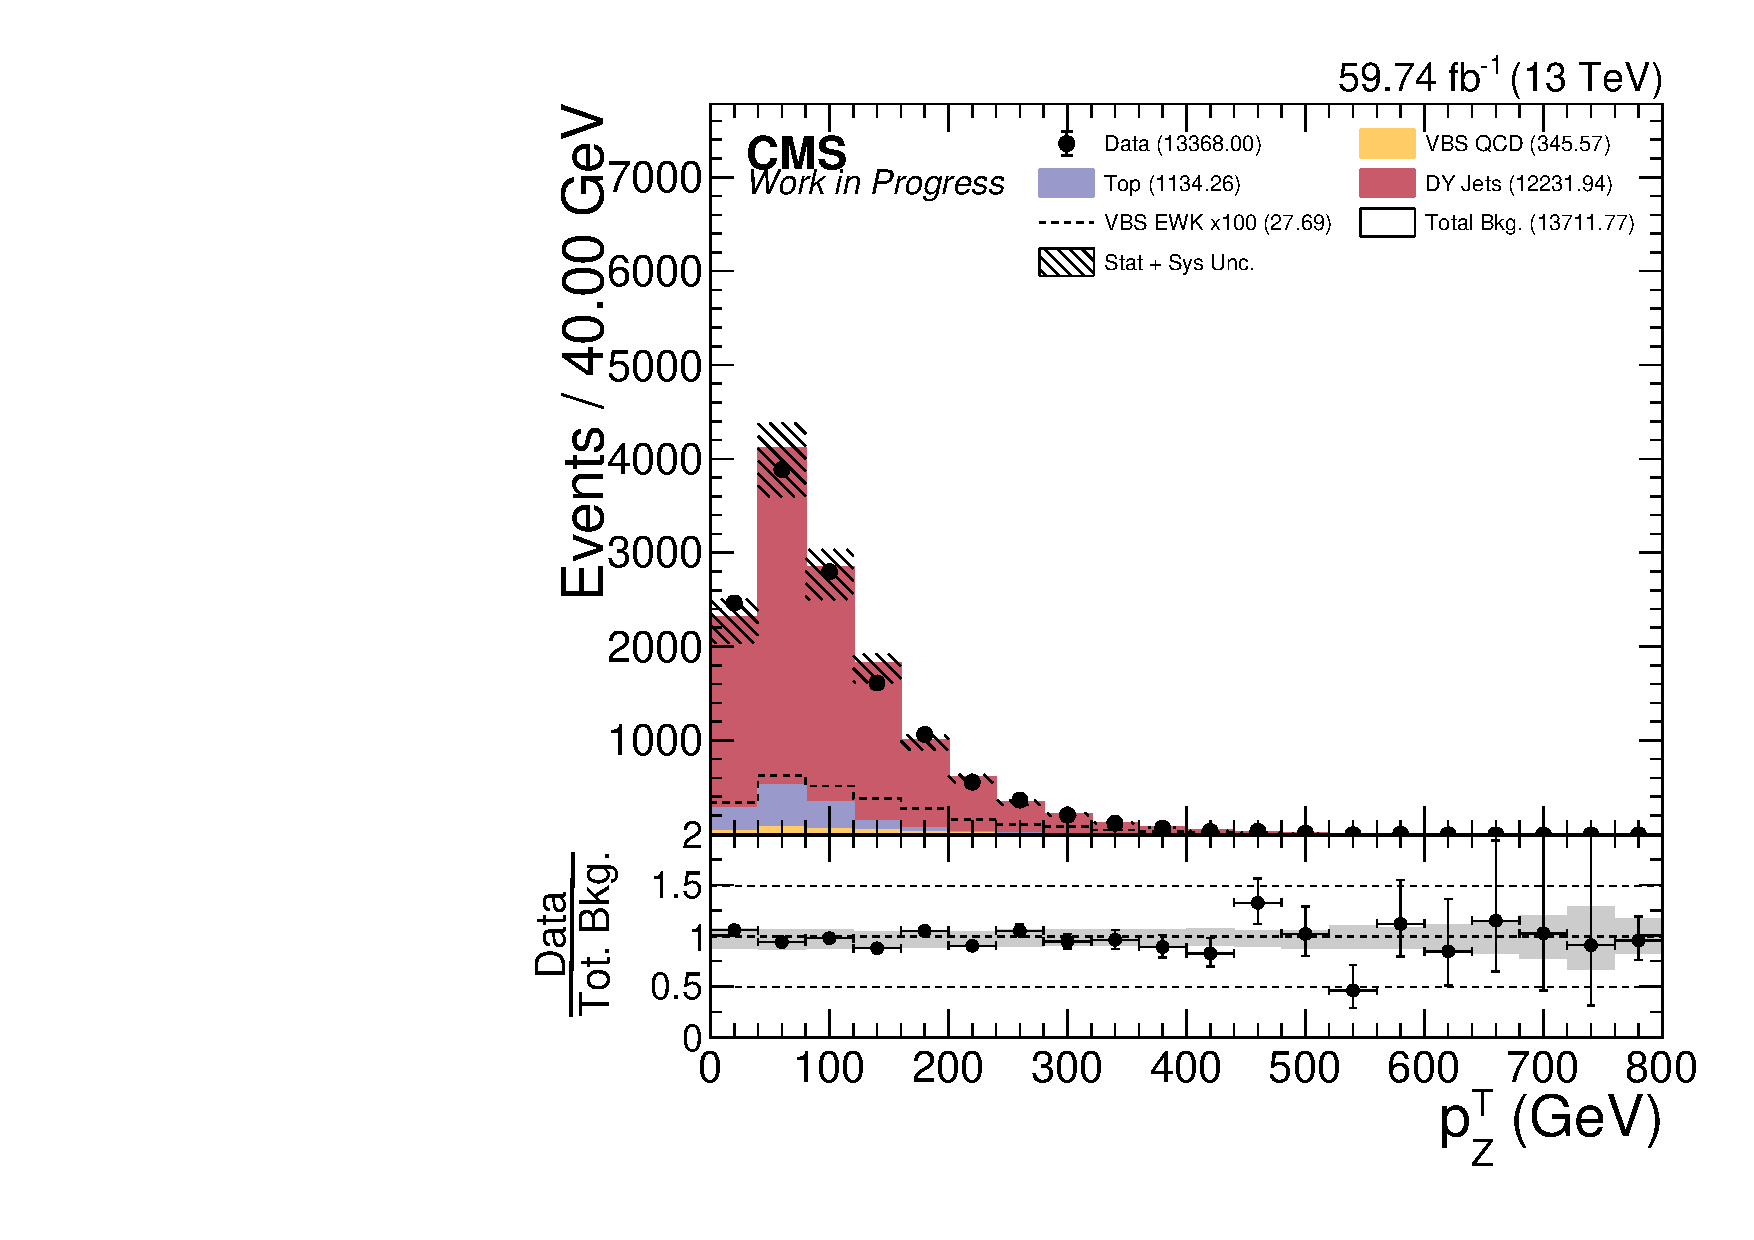
\includegraphics[width=0.335\textwidth]{analysis_plots/2018_zjj/cr_vjets_l/v_lep_pt.pdf} \hspace{-10pt} \\
  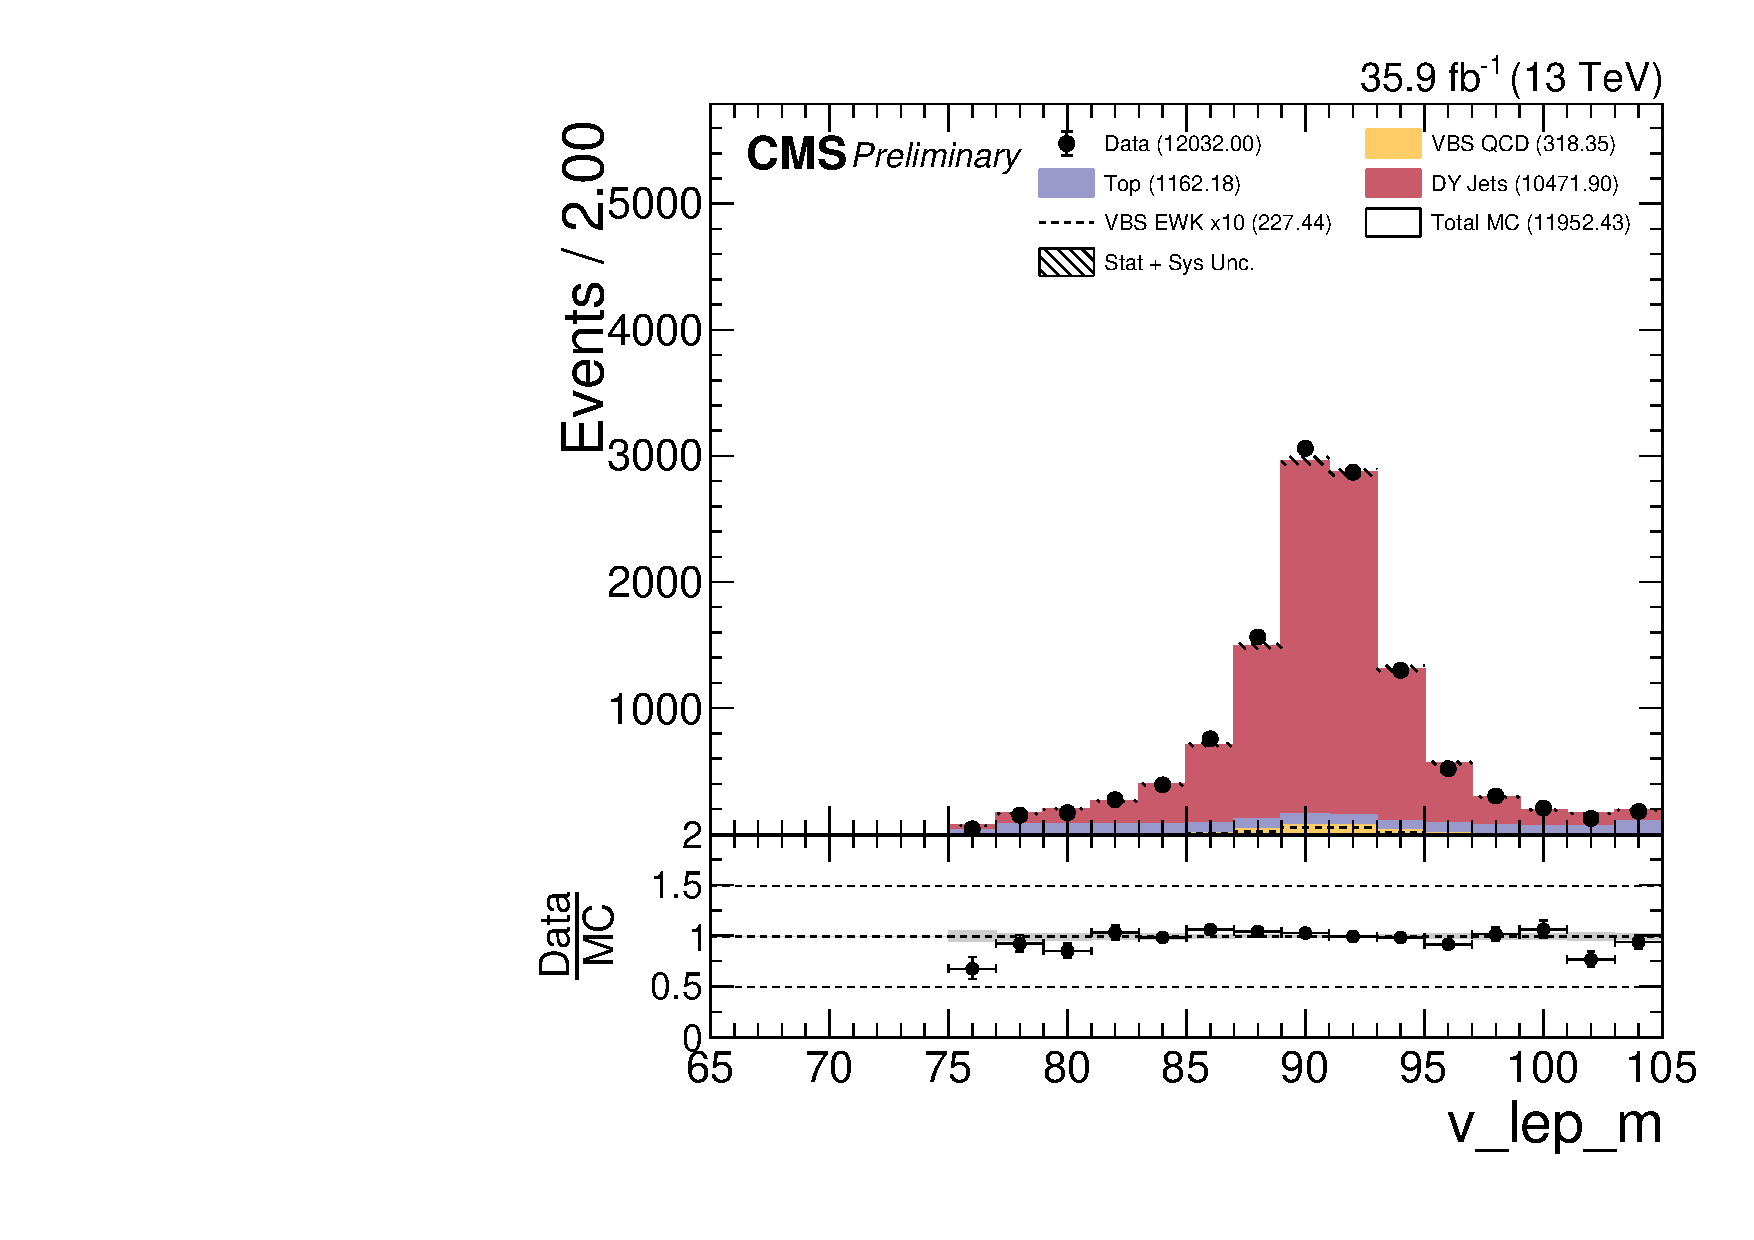
\includegraphics[width=0.335\textwidth]{analysis_plots/2016_zjj/cr_vjets_l/v_lep_m.pdf} \hspace{-10pt}
  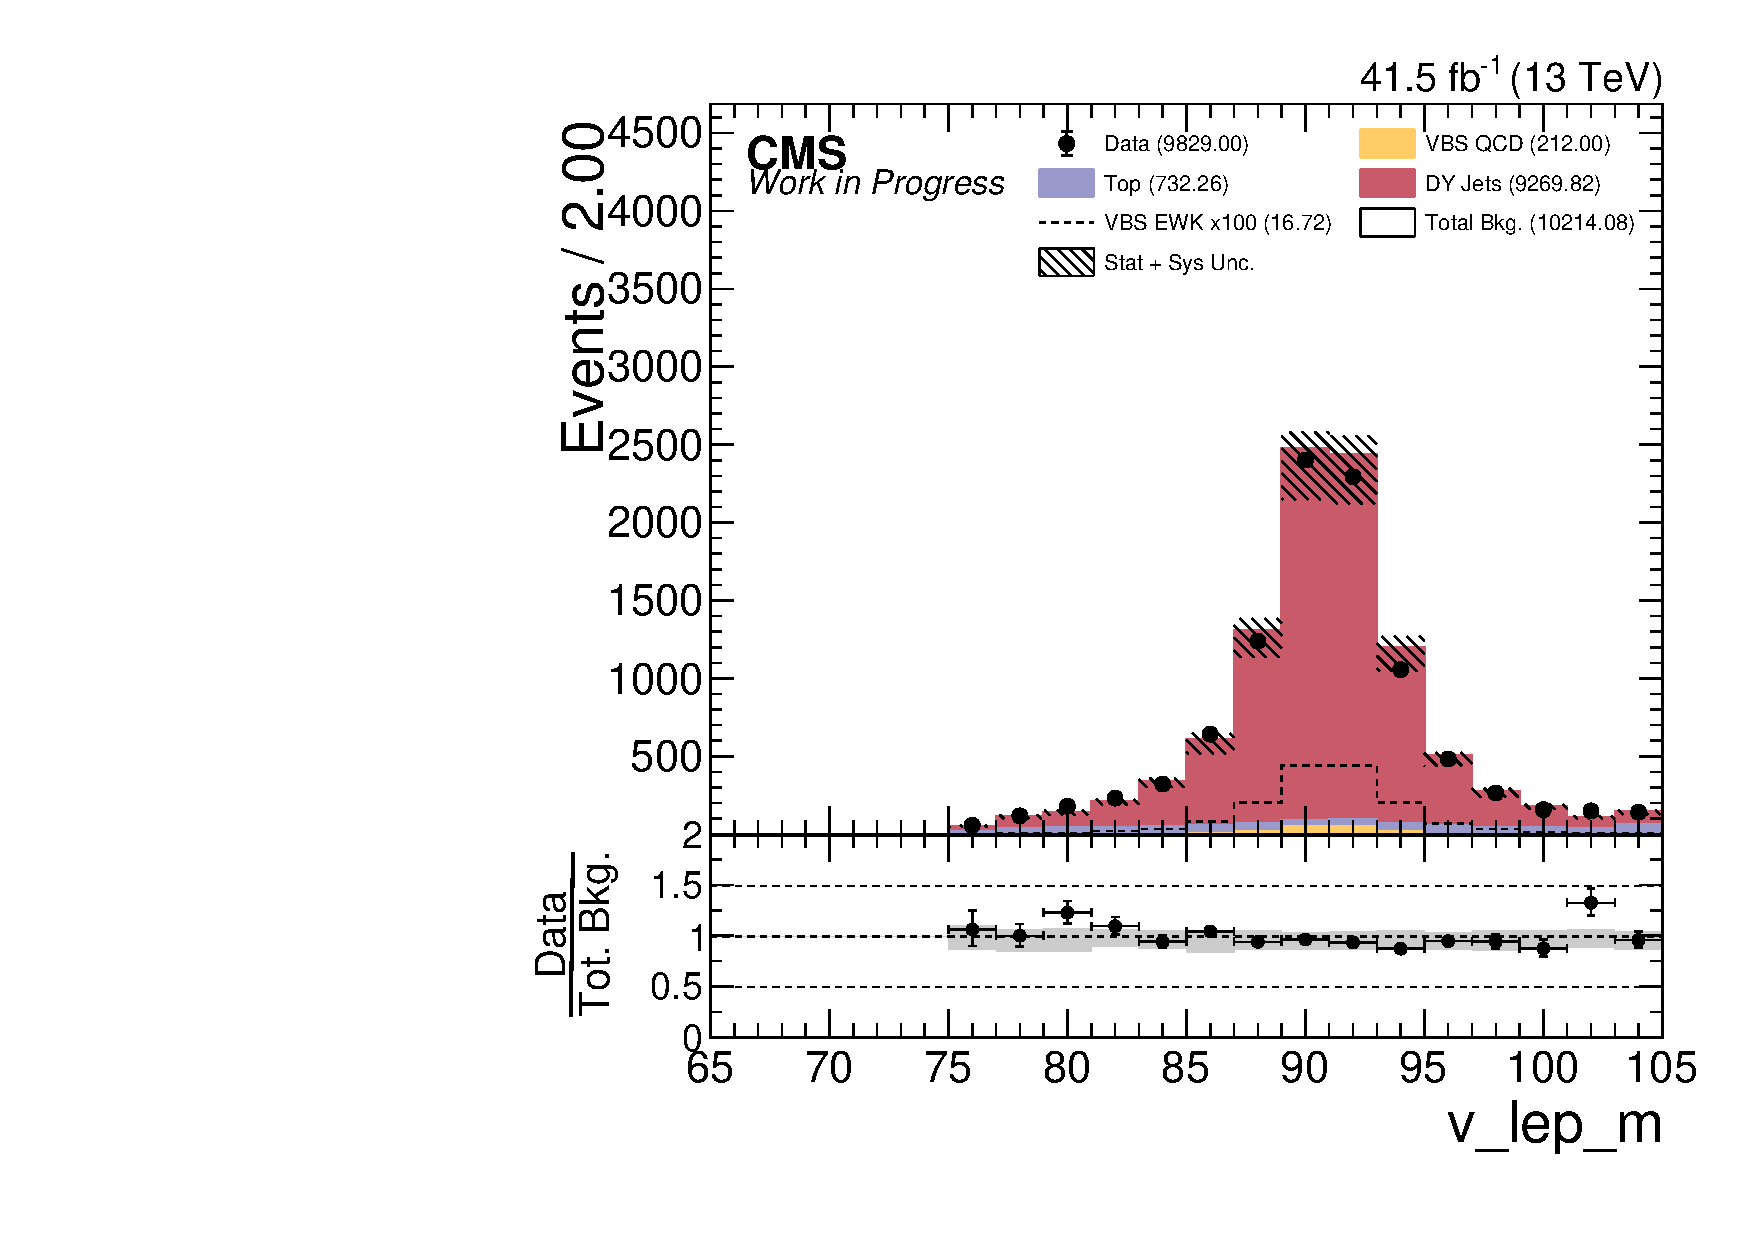
\includegraphics[width=0.335\textwidth]{analysis_plots/2017_zjj/cr_vjets_l/v_lep_m.pdf} \hspace{-10pt}
  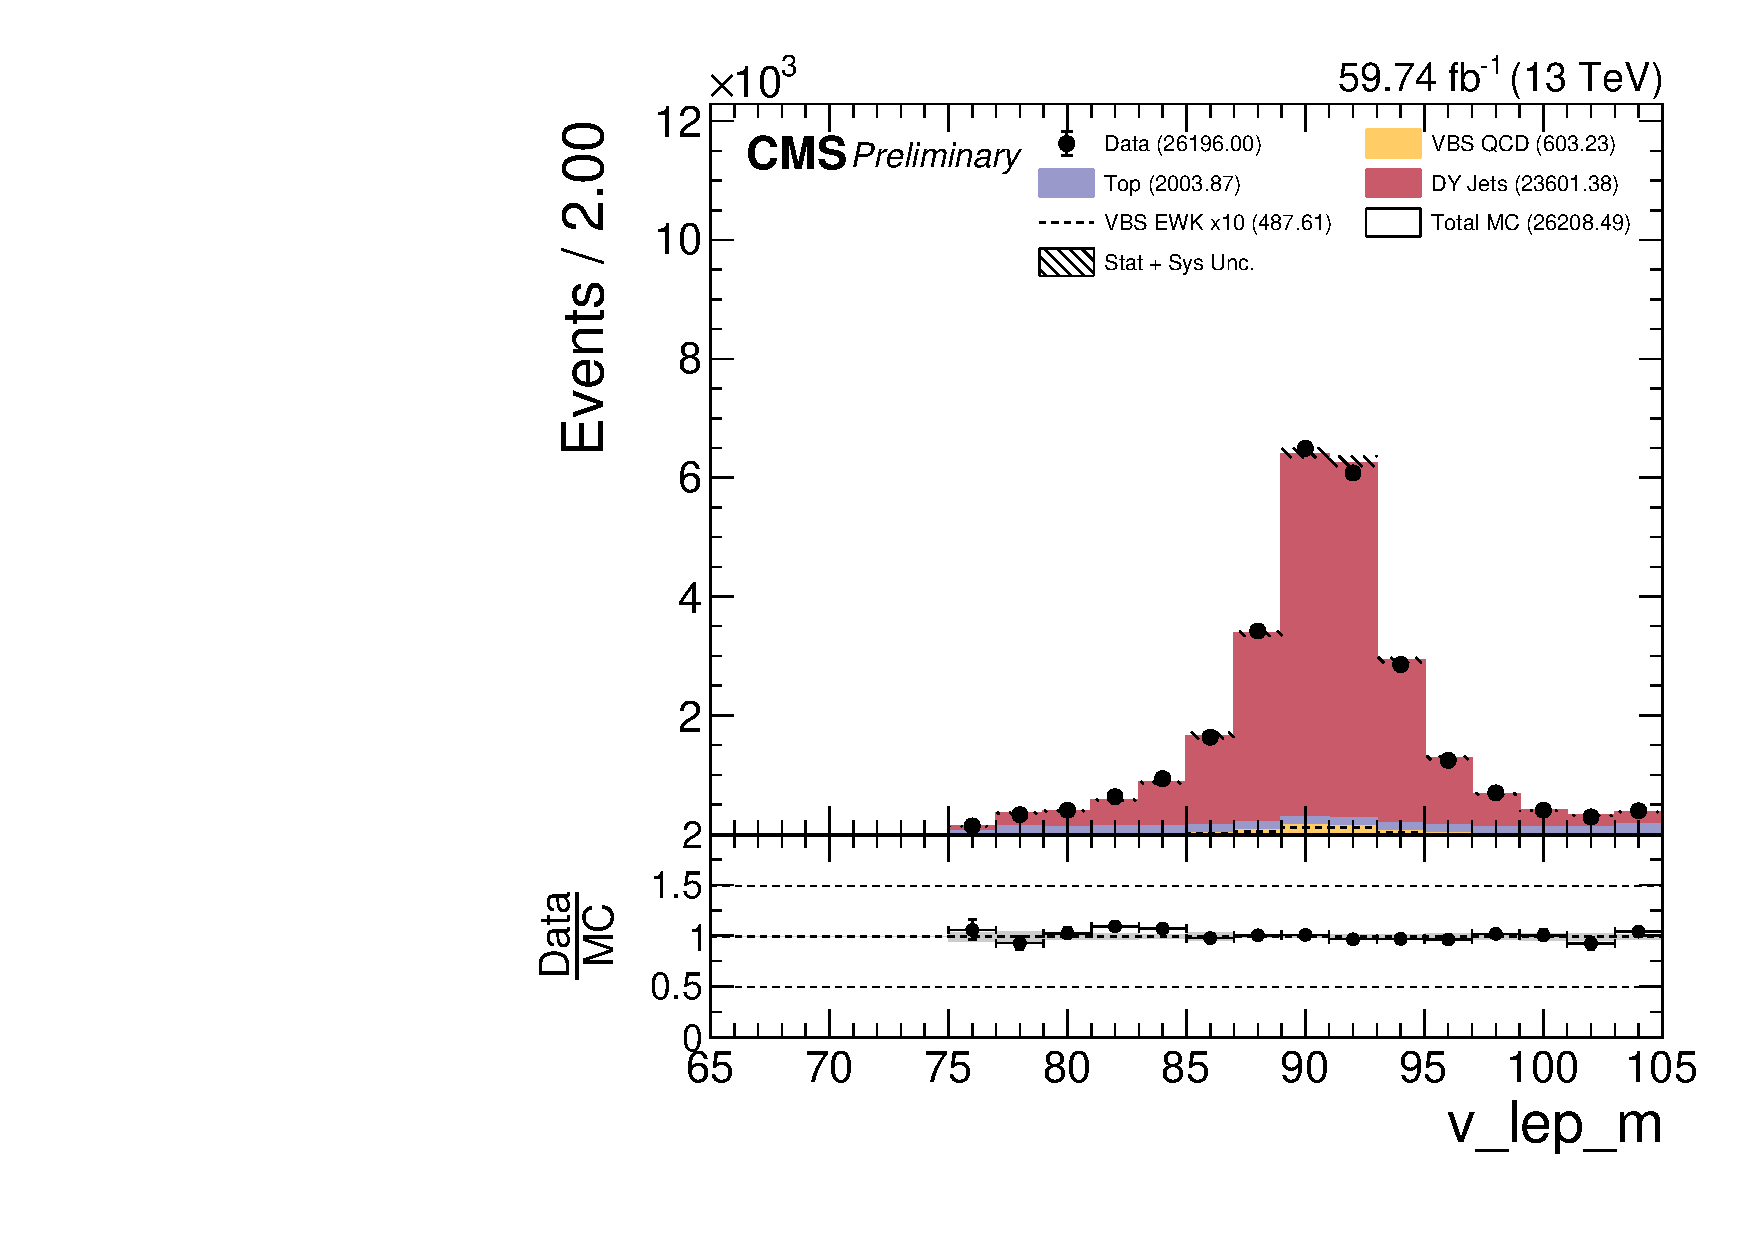
\includegraphics[width=0.335\textwidth]{analysis_plots/2018_zjj/cr_vjets_l/v_lep_m.pdf} \hspace{-10pt} \\
  \caption[DY+Jets Control Region: \textit{Z} boson kinematics in Resolved ZV Channel]%
  {DY+Jets Control Region: \textit{Z} boson kinematics in Resolved ZV Channel.
    Error bars include statistical uncertainty on total background,
    JES and QCD scale systematic on DY+Jets and VBS\_QCD MC\@. From Left to Right: 2016,
    2017, and 2018. From Top to Bottom: \( p_T \), and mass.}%
  \label{fig:zjj-cr-vjets-l-v-lep-pt-m}
\end{figure}


\begin{figure}[!ht]
  \centering
  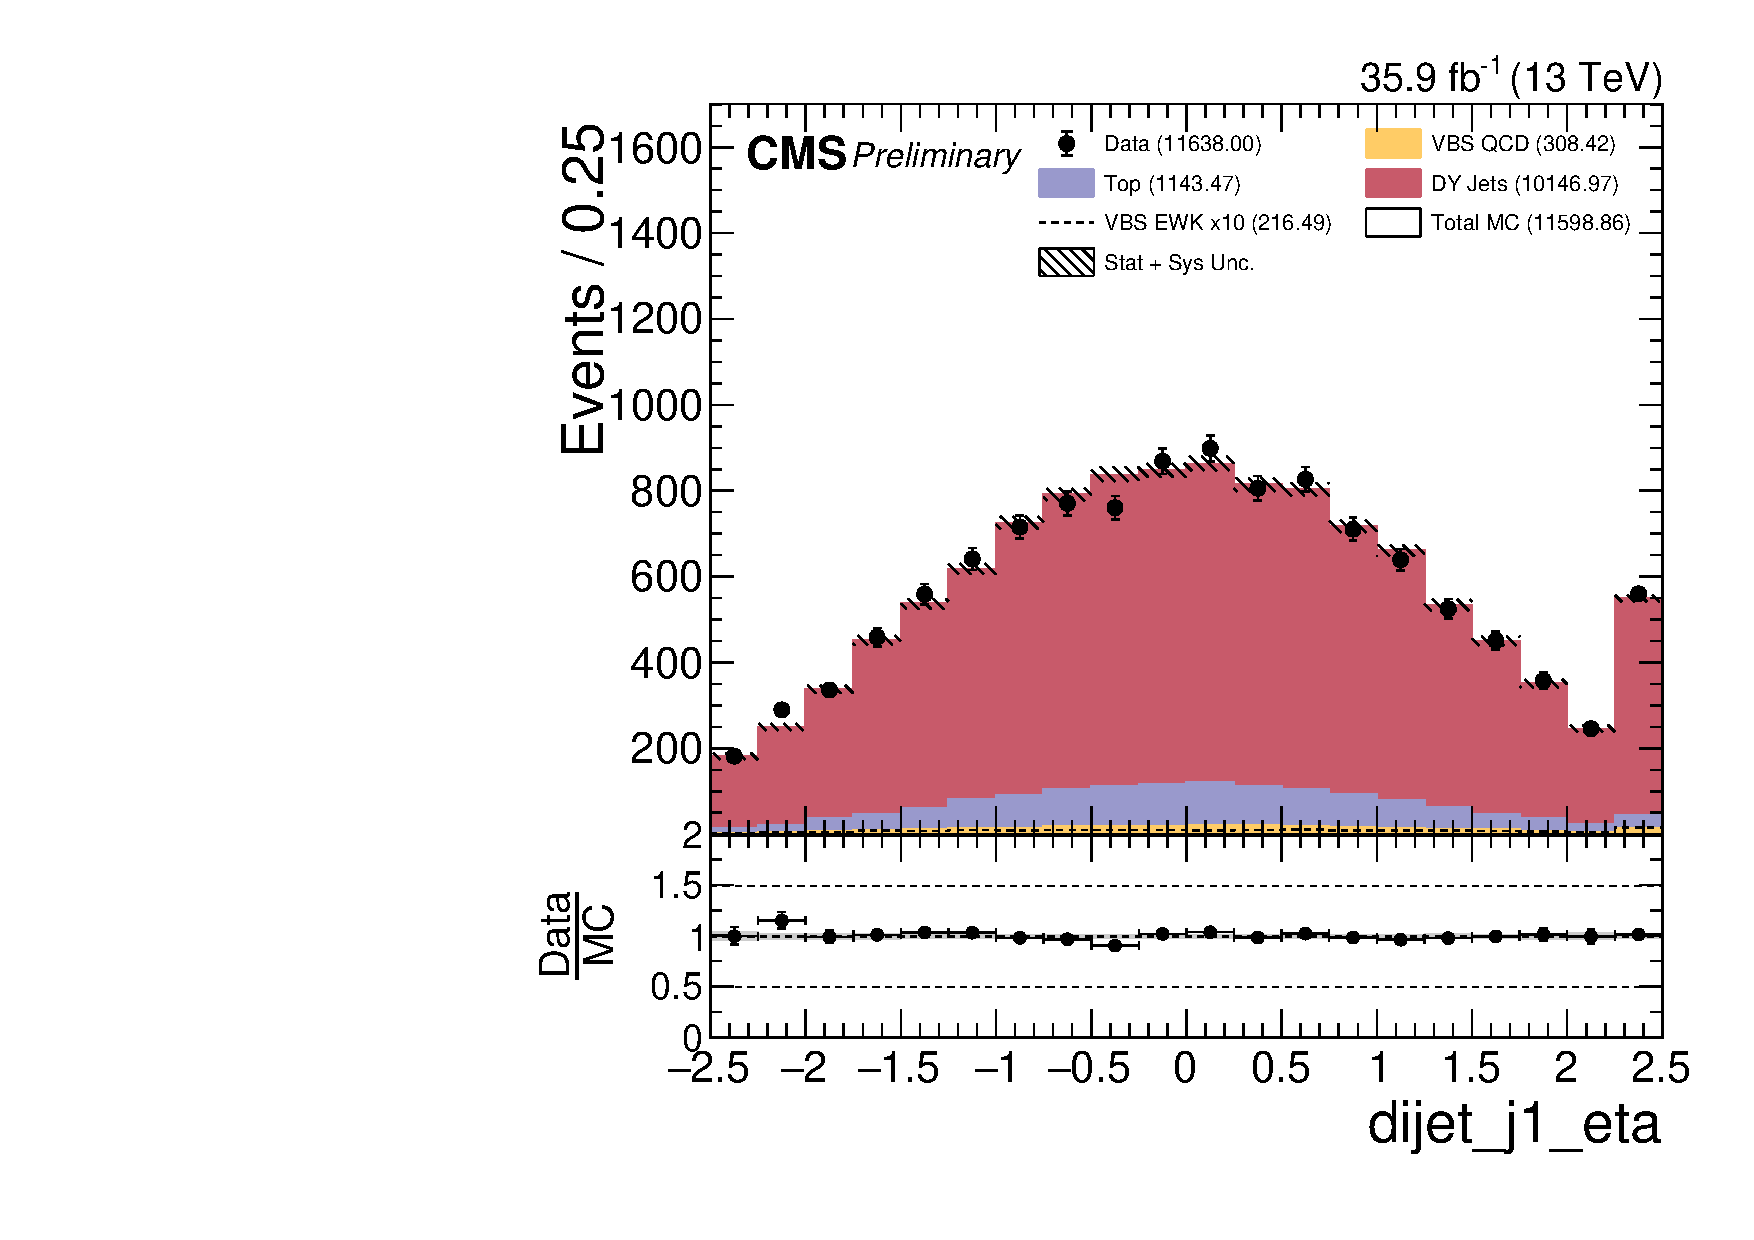
\includegraphics[width=0.335\textwidth]{analysis_plots/2016_zjj/cr_vjets_l/dijet_j1_eta.pdf} \hspace{-10pt}
  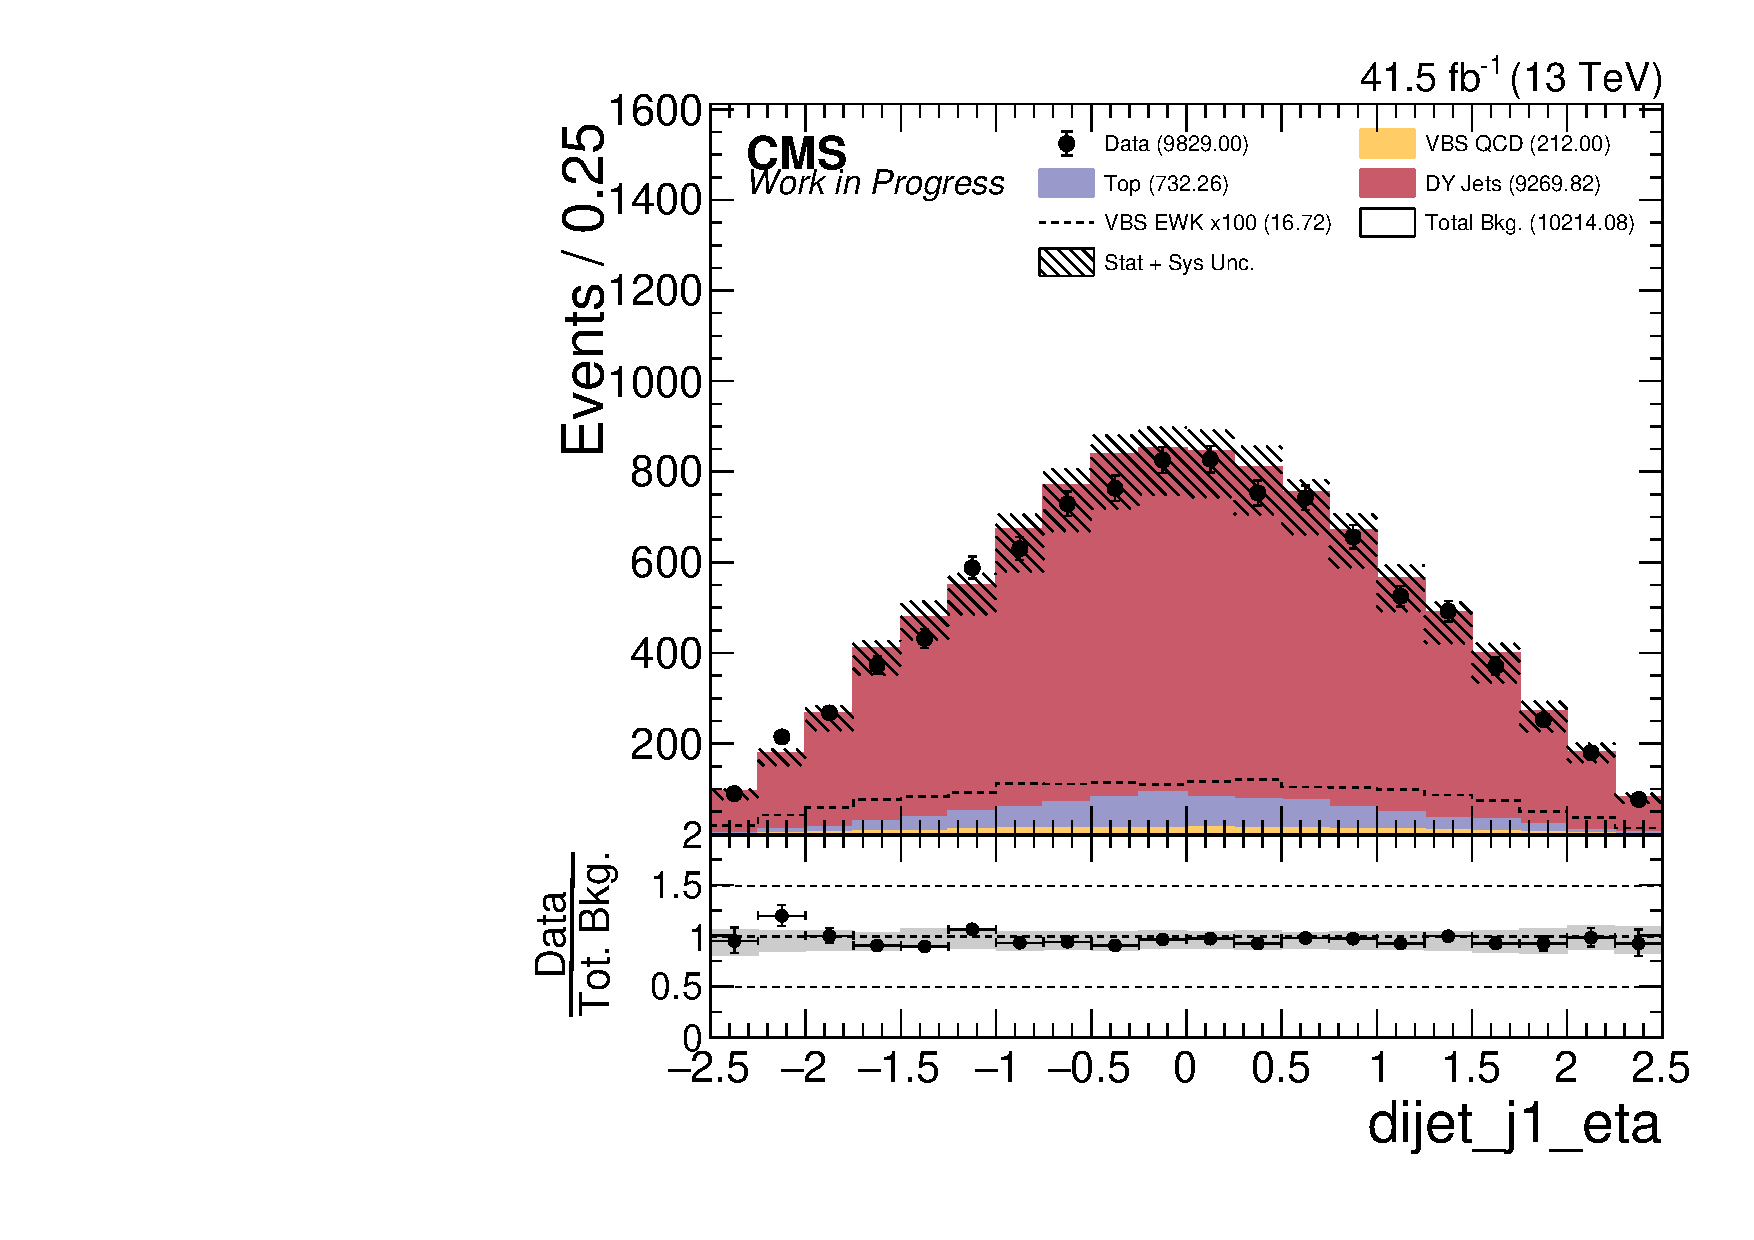
\includegraphics[width=0.335\textwidth]{analysis_plots/2017_zjj/cr_vjets_l/dijet_j1_eta.pdf} \hspace{-10pt}
  \includegraphics[width=0.335\textwidth]{analysis_plots/2018_zjj/cr_vjets_l/dijet_j1_eta.pdf} \hspace{-10pt} \\
  \includegraphics[width=0.335\textwidth]{analysis_plots/2016_zjj/cr_vjets_l/dijet_j2_eta.pdf} \hspace{-10pt}
  \includegraphics[width=0.335\textwidth]{analysis_plots/2017_zjj/cr_vjets_l/dijet_j2_eta.pdf} \hspace{-10pt}
  \includegraphics[width=0.335\textwidth]{analysis_plots/2018_zjj/cr_vjets_l/dijet_j2_eta.pdf} \hspace{-10pt} \\
  \caption[DY+Jets Control Region: \textit{V} boson leading and trailing jet \( \eta \) in Resolved ZV Channel]%
  {DY+Jets Control Region: \textit{V} boson leading and trailing jet \( \eta \) in Resolved ZV Channel.
    Error bars include statistical uncertainty on total background,
    JES and QCD scale systematic on DY+Jets and VBS\_QCD MC\@. From Left to Right: 2016,
    2017, and 2018. From Top to Bottom: \( \eta \) of leading jet, and \( \eta \) of trailing jet.}%
  \label{fig:zjj-cr-vjets-l-dijet2-pt-eta-m}
\end{figure}

\clearpage
\section{
  Impact Plots
 }\label{app2:impact-plots}

\begin{figure}[!ht]
  \centering
  \includegraphics[width=\textwidth,page=3]{analysis_plots/impact_plots/impacts_datacard_run2_z.pdf}
  \caption{Impact Plots of nuisance parameters from 61 to 90.}\label{fig:vbs-impact-plots-page3}
\end{figure}

\begin{figure}[!ht]
  \centering
  \includegraphics[width=\textwidth,page=4]{analysis_plots/impact_plots/impacts_datacard_run2_z.pdf}
  \caption{Impact Plots of nuisance parameters from 91 to 110.}\label{fig:vbs-impact-plots-page4}
\end{figure}
